\documentclass[12pt,a4paper]{report}
\usepackage[english]{babel}
\usepackage{newlfont}
\usepackage{color}
\usepackage[autopunct=true]{csquotes}
%\usepackage{quotchap} for different chapters titles layout
\usepackage{epigraph}
\usepackage{bm}%to make math symbols in bold style.
\usepackage{hyperref} %hyperlinks
\usepackage{graphicx} %figures
\usepackage{amsmath} %math
\usepackage{amsfonts} %to do the bold W
\usepackage{mhchem}
%\usepackage[toc,page]{appendix}
\usepackage{fancyhdr}%Add chapter name at the beginning of each page
%\pagestyle{fancy}
\setlength{\headheight}{15pt}% ...at least 51.60004pt

\usepackage[]{lineno} %Professor  
\runninglinenumbers



\usepackage[titletoc,title]{appendix}
\usepackage{float} %to force position of figures
\usepackage{mathtools}
\usepackage{unicode-math}
%\usepackage[notindex]{tocbibind} you will no longer need to provide the instruction \addcontentsline{toc}
\usepackage[nottoc]{tocbibind}%to remove contents from table of contents and to add bibliography to it.
\renewcommand*\footnoterule{}

\usepackage{tocloft} %to personalize table of contents
% Update \subsections in ToC
%\renewcommand{\cftsubsecleader}{~}% Content between subsection title and page number
%\renewcommand{\cftsubsecafterpnum}{\hfill\mbox{}}% Content after subsection page number
\cftsetrmarg{12em}    
\renewcommand{\cftpnumalign}{l} % left aligned page numbers

\usepackage{caption}    
\captionsetup[figure]{hangindent=0pt, singlelinecheck=false}


\usepackage[flushmargin]{footmisc}

%\usepackage[nottoc]{tocbibind} To add sections in the table of contents 
\textwidth=450pt\oddsidemargin=0pt

\newcommand{\pyobject}[1]{\fbox{\color{red}{\texttt{#1}}}}


\begin{document}
\begin{titlepage}
%
%
% ONCE YOU ARE FINISHED WITH YOUR CHANGES MODIFY "RED" WITH "BLACK" IN ALL \textcolor COMMENTS
%
%
\begin{center}
{{\Large{\textsc{Alma Mater Studiorum $\cdot$ University of  Bologna}}}} 
\rule[0.1cm]{15.8cm}{0.1mm}
\rule[0.5cm]{15.8cm}{0.6mm}
\\\vspace{3mm}
{\small{\bf School of Science \\
Department of Physics and Astronomy\\
Master Degree in Physics}}
\end{center}

\vspace{23mm}

\begin{center}\textcolor{red}{
%
% INSERT THE TITLE OF YOUR THESIS
%
{\LARGE{\bf THESIS TITLE}}\\
}\end{center}

\vspace{50mm} \par \noindent

\begin{minipage}[t]{0.47\textwidth}
%
% INSERT THE NAME OF THE SUPERVISOR WITH ITS TITLE (DR. OR PROF.)
%
{\large{\bf Supervisor: \vspace{2mm}\\\textcolor{red}{
Prof./Dr. Name Surname}\\\\
%
% INSERT THE NAME OF THE CO-SUPERVISOR WITH ITS TITLE (DR. OR PROF.)
%
% IF THERE ARE NO CO-SUPERVISORS REMOVE THE FOLLOWING 5 LINES
%
\textcolor{red}{
\bf Co-supervisor: (optional)
\vspace{2mm}
Prof./Dr. Name Surname\\\\}}}
\end{minipage}
%
\hfill
%
\begin{minipage}[t]{0.47\textwidth}\raggedleft \textcolor{black}{
{\large{\bf Submitted by:
\vspace{2mm}\\
%
% INSERT THE NAME OF THE GRADUAND
%
\textcolor{red}{
Name Surname}}}
}
\end{minipage}

\vspace{40mm}

\begin{center}
%
% INSERT THE ACADEMIC YEAR
%
Academic Year \textcolor{red}{ 201*/201*}
\end{center}

\end{titlepage}


\newpage
\thispagestyle{empty}
\mbox{}
\newpage





\thispagestyle{empty} %remove the page number
 \epigraph{``Behind the great achievements of a Gauss or an Einstein is in all cases a life devoted to contemplation, curiosity, collaboration and, perhaps most of all, hard work.
''\footnotemark}{Brian D. Burrell, Professor of Neuroscience}
\footnotetext{GENIUS IN A JAR, Scientific American 2015 Sep; 313(3):82-7.}




\newpage
\thispagestyle{empty}
\mbox{}
\newpage

\thispagestyle{empty}
\begin{flushright}
 Dedica.
\end{flushright}

\newpage
\thispagestyle{empty}
\mbox{}
\newpage


\begin{flushleft}
{\LARGE{\bf Abstract}}\\
\vspace{9mm}
I hope it will be an important thesis.
%I tre principali circuiti analizzati sono semplici da modellizzare per� rappresentano importanti sistemi biologici e la loro simulazione e analisi non � affatto banale: serve anche qui molto succo di cervello e fantasia per poter svelare importanti caratteristiche che tali sistemi nascondono. I risultati ottenuti possono essere sfruttati in sistemi pi� articolati come l'NF-kB che � il nostro target. 
%Chronic diseases, cancers and diabetes are associated with dysregulation of many biochemical cues. These biochemical cues are proteins that regulate cellular activity migration and death. The synthesis of these proteins is regulated by nuclear transcription factors. One of the most studied transcription factor is nuclear factor kappa B (NF?B). Many different proteins have been identified that regulate the activity of NF?B. Yet, how these proteins regulate NF?B is still unclear (Dalla tesi di Huanling Liu).
%(dalla lezione del 15/10/2018)
%And of course if you change these constants you will have different behaviors. So an other step will be to learn how to play with the parameters because this is a huge problem in modeling. The usual problem is how to find the parameters numbers. This is not trivial and there are some possibilities that I will show in the next lecture.
%transcription factors have functional properties because they interfere in some biological process.
%In order to regulate the RNA production, nature invented the transcription factors.
%La nostra modellizzazione dell'NF-kB � molto semplificata e ideale tipo ideal gas o Michaleis-Mentein reaction.
\end{flushleft}
\thispagestyle{empty}
\clearpage
\pagenumbering{arabic}
%to reset the page number.

\newpage

\tableofcontents

\newpage



%First part: introduction into heterogeneity and how to deal with it using physical methods.
\part{Introduction into biological stochasticity and physical methods for its investingation}

\pagestyle{fancy}
\makeatletter% Needed because of @ in macro name ? https://tex.stackexchange.com/q/8351/277964
\renewcommand{\chaptermark}[1]{%
  \markboth{\@chapapp \thechapter\ --\ #1}{\@chapapp \thechapter\ -- \ #1}% chapter/appendix name and number moved from \fancyhead[L]{�}
}
\makeatother% because of \makeatletter before
\fancyhead[R]{}
\fancyhead[L]{\leftmark}% chapter/appendix name and number moved to \chaptermark

\chapter{Introduction}\epigraph{``Frase''}{Autore}



Kevin Burrage et al. in their important paper \emph{Stochastic simulation in systems biology} \cite{Article} highlight how mathematical modelling and computational simulation perform essential roles in biology. Models are useful for many different purposes: perhaps the most important of these are crystallising our assumptions and testing them, guiding experiments and looking at experimentally unreachable scenarios, as well as the much-vaunted ability to make new predictions. 

Ideally, there should be a virtuous cycle between experiment and theory to understand the natural system in which we are interested. If the model and experiments agree, then parameters for the model can be inferred from the data and the model refined, again leading to further experiments.  If they do not agree, this implies that the hypothesis was inappropriate: the model needs revision, and theoretical tests using different models can provide a starting point for further experiments. For this we need to go back to our natural system and propose revisions (major or minor) to the model and new avenues for experiment.

As defined by Kevin Burrage et al., model is an abstract representation of the system in which we are interested and this is usually formulated mathematically. This model can, in simple cases, be solved analytically for a particular question, giving us an \emph{exact} analytical solution to the question posed to the model. In general, however, analytical solutions for all but the most simple models do not exist, and we need to use methods to solve the model numerically. These last methods give rise to numerical solutions which are approximations to the analytical solution.% that become more and more accurate as we use smaller and smaller numerical steps (the unit of discretisation of a numerical approach)

In many cases, the numerical solution will try to mimic the behaviour of the real system over time: this is a simulation.

An important point to remember when we talk about mathematical models is that, in a sense, ``all models are wrong''  but this does not mean their conclusions or predictions are false, as the famous quote continues, ``but some are useful''. Rather, we should bear in mind that all models are abstractions of reality, simplified versions of the real systems that they represent. A model is a vehicle for gaining understanding, and we would not gain any new understanding from a model that was as complicated as the real system. 

Almost all models are phenomenological; that is, they are based on a set of simplified assumptions that we have distilled from the real system using intuition rather than rigorous proof from basic principles. Incorporating only the important ones allows us to crystallise our understanding of the system (and if the model gives wrong results, we know that our assumptions were wrong or incomplete, hence it is in any case a gain in knowledge of our system under study). Creating phenomenological models is not a trivial task: ``sensing which assumptions might be critical and which irrelevant to the question at hand is the art of modeling''. The choice of what to include in the model lies with the modeller.
%Dipende da: the choice of modelling/simulation method is determined by the aspects of the natural system in which we are interested, how realistic an estimation of it we want, and our mathematical and computational resources.

%Importanza dei modelli tipo quello SIR oggigiorno.

%Simulation modeling activities encapsulate all three major modeling methods of data analytics: descriptive, predictive, and prescriptive. Descriptive modeling uses historical data to describe what happened in order to understand past behavior of a system. Predictive modeling uses historical data to develop models that help us understand future behavior in order the answer what may happen. Descriptive modeling summarizes past data for understanding. Predictive modeling uses past data to predict future behavior. Prescriptive modeling indicates what should be done and is integral to answering questions involving system design.+finale https://rossetti.github.io/RossettiArenaBook/why-simulate.html



\section{Heterogeneity in biology}
Stochastic computational methods have become commonplace in science because they are able to appropriately account for one key feature in biology: this is heterogeneity.

There are three different sources of heterogeneity in natural systems: genetic, environmental (i.e. also known as \emph{extrinsic noise}) and stochastics (i.e. also called \emph{intrinsic noise}).

Genetic heterogeneity occurs through the production of single or similar phenotypes through different genetic mechanisms \cite{GeneticHeterogeneity}. The general ``rule'' in biology is that cells and animals with different genes should clearly be different in phenotypes. However, the so called ``convergent evolution'' represents an exception to this rule where different species evolved similar phenotypic features independently. This phenotypic similarity is thought to usually have a different genetic basis, showing that the relationship between genotype and phenotype is not a simple, linear one \cite{genotypevsphenotype}. 

On the other hand, even isogenic (that is, genetically identical) organisms or populations of cells can be very different; the famous cloned animals are excellent illustrations of this phenomenon, known as non-genetic or phenotypic heterogeneity. Daniel Stockholm et al. in their work named \emph{The Origin of Phenotypic Heterogeneity in a Clonal Cell Population In Vitro}\cite{heterogeneityinclones} show phenotypic switch in initially identical cells. This suggests that heterogeneity is not only generated by genetic variation but it is triggered by two other factors.

The first one is the consequence of \emph{extrinsic factors}: initially identical cells may become different because they encounter different local environments that induce adaptive responses. Examples of each of these factors could be: if we were interested in animal populations, the weather an animal experiences in a particular year or if we were interested in levels of protein expression of a cell population, we might look at differences in individual cells such as ribosome number and cell cycle stage.

The third source of heterogeneity is instead \emph{intrinsic} to cells and may occur even in homogeneous environments. Indeed identical genotype and environmental exposure are not sufficient to guarantee a unique
phenotype. The intrinsic heterogeneity is present in all living (and non-living) systems but often masked by the macroscopic scale at which we observe them. Spudich and Koshland were perhaps the first to observe this in a cell biology context. As explained in their paper \emph{Non-genetic individuality: chance in the single cell} \cite{intrinsic}, they noticed that individual bacteria from an isogenic population maintained different swimming patterns throughout their entire lives. This was a visible manifestation of the third source of heterogeneity: \emph{chance}, otherwise known as \emph{stochasticity} or \emph{intrinsic heterogeneity} (often interchangeably called \emph{intrinsic noise}). 

This arises from random thermal fluctuations at the level of individual molecules. It affects the DNA, RNA, protein and other chemical molecules inside cells in many ways, most notably by ensuring that their reactions occur randomly, as does their movement (via Brownian motion). Very clear examples could be the following: consider a single mother cell dividing into two daughter cells of equal volume. During the division process, all the molecules in the mother cell are in Brownian motion according to the laws of statistical mechanics. The probability that each daughter cell inherits the same number of molecules is infinitesimally small. Even in the event that the two daughter cells receive exactly one copy of a particular transcription factor, each transcription factor will perform a Brownian random walk through its cellular volume before finding its target promoter and activating gene expression. Because Brownian motion is uncorrelated in the two daughter cells, it is statistically impossible for both genes to become activated at the exact same time, further amplifying the phenotypic difference between the two daughter cells. These are just two examples of the many sources of gene expression
variability that arise in isogenic cells exposed to the same environment \cite{geneexpressionnoise}.

 Intrinsic heterogeneity is inherent to the process of gene expression and cannot be predicted (except in a statistical sense) or fully eliminated. Thus two identical genes in an identical intracellular environment would still be expressed differently, even in the absence of the previous two sources of heterogeneity.
 
 Hence, the reason of terminologies is clear: we talk about extrinsic heterogeneity because it arises from other, outside, sources and affects all genes inside a cell equally, whereas the random fluctuations are actually inherent to the expression of a single gene.
 
 It is important to point out that these three sources of heterogeneity are not independent because they are all interconnected in their effects on cells and populations. For instance, cellular decision involves both environmental and intrinsic heterogeneity, the former in affecting which stable states are possible and the latter in switching between them.
 
 Another example is that of genetic mutations, where intrinsic noise causes the mutations that then contribute to genetic heterogeneity and so causing genetic mutations that are essential for creating the heritable variation, thus allowing evolution to occur.
 
 From this, a very interesting example of the interplay of all three types of heterogeneity is evolution, one of the most fundamental processes in nature: evolution acts on phenotypes, which have a genetic basis but are also affected by both extrinsic and intrinsic noise. Studying how evolution shapes noise is a key challenge and this is highlighted in the work \emph{Adaptive noise} by M. Viney et al. \cite{adaptivenoise}. If our DNA is much different from the first humans appeared on Earth (and so also our phenotype), is due to all this complex interplay among sourcies of heterogeneities.
 
Finally focusing on intrinsic heterogeneity, we have to point out how this can be a double-edged sword: intrinsic noise has both positive and negative influence that have to be accounted for cells and organisms. One positive effect is already mentioned: it allows evolution to occur. One other related example is that some biological systems have evolved to make use of it: for instance, in the case of persister-type bacteria, which form a subset of some bacterial populations and can withstand antibiotic treatments even though they do not have genetic mutations for resistance. This is an example of cellular decision making, the ability of cells to randomly transition between different stable, heritable states.

Some of the most well-known examples of cellular decision making are bacteria, and yeast, which are easier to investigate experimentally than large multicellular organisms. Yet, this phenomenon is common to cells at all levels of life and is argued to be one of the key processes in cellular development. The main difference is that in unicellular organisms, cellular decision making is useful for cheap, non-genetic adaptation in the face of fluctuating environments, whereas in multicellular organisms it is used to produce distinct cell types and functions within a constant environment.

Intrinsic noise is also an interesting object of study since it represents a ``fingerprint'' with which to explore fundamental questions on mechanisms and dynamics of gene regulation by means of measurements of cell-to-cell variability in gene expression \cite{geneexpressionnoise}.

However, as said before, intrinsic noise causes mutations which can also have negative effects. Deleterious mutations that are phenotypically expressed frequently result in loss of important functions or even organismic death, and it has been shown that a substantial proportion of mutations are deleterious. Mutations are also thought to cause cancer, which has become a serious disease in modern times. %in stem and somatic cells
 
 %+la parte che parla degli effetti positivi e negativi della regolazione ed il fatto che tutte le eterogeneit� sono interconnesse.



%Il fatto che cellule diverse possono avere stesso patrimonio genetico porta a pensare che non esiste solo il genetic heterogeneity bens� la causa di questa diversit� fenotipica pu� essere data dall'environment e dal caso.



%Partiremo dai circuiti genetici pi� semplici fino ad arrivare all'NF-kB.
%Magari prova ad iniziare con la frase ``We and all other animals are machines of our genes''. Originally published in 1976, Richard Dawkins' book argues that genes are the basic unit of evolution, not individual organisms or even species. Due to their naturally selfish behavior, genes merely use organisms as mechanisms to ensure their own survival.
%Però ci sono processi come quelli descritti nell'articolo using gene expression noise for understanding gene regulation che dimostrano che i nostri geni non sono tutto.
%Single-cell experiments.
%Su cosa tratterà l'intera tesi.
%Il nostro DNA cambia stando a contatto con l'ambiente: gli uomini del passato lo avevano diverso dal nostro e lo si vede dall'aspetto (fenotipo).

%Da stochastics simulations in biological systems.
%In this thesis, we will refer to reactions occuring inside a cell volume between different types of biochemical molecules with various reaction rates. These will generally be genes , i.e. sections of DNA that are copied into mRNA and initiate a gene expression network, RNA or proteins. 

\section{Colonrectal cancer (CRC)}
%Il background biologico con i concetti di base come gene regulation.+%Randomness è anche nell'iniziazione del tumore al CRC: il 70% dei tumori avvengono in maniera sporadica e secondo il modello genetico di Fearon si ha una prima mutazione che colpisce un tumor-suppressor gene, adenomatous polyposis coli (APC) initiating colorectal tumorigenesis. Il 30% ha base familiare.

\section{Deterministic versus stochastic models}
Before the discovery of intrinsic noise, mathematical and computational methods that have traditionally been used were typically \emph{systems of differential equations} which are both \emph{continous} and \emph{deterministic}, i.e. their state variables are real numbers representing the concentrations of molecules and they do not include noise.

Such models can be considered as accurate only when we are interested in the mean dynamics of a large number of molecules, large enough that we need not worry about individual molecules but can approximate them as concentrations \cite{Article}. Above a molecular population size of the order of many hundreds or above, the fluctuations from intrinsic noise are averaged out and the deterministic approximation becomes increasingly valid.

This is because intrinsic noise, as a rule of thumb, behaves as $\frac{1}{\sqrt{X}}$ , where \emph{X} is the number of molecules in the system. This is confirmed by experimental studies that find that total noise does scale roughly as the inverse square of abundance until high abundances. At this point, extrinsic noise is thought to take over as the dominant source of noise \cite{noisewithabundance}.

Therefore, it often becomes necessary to include the effects of stochasticity in biological models, especially for small systems with low populations of some molecular species, such as \emph{gene expression networks}. Here, \emph{discrete stochastic models} must be used, whose variables represent actual molecular numbers.

In the cellular environment, the reactant numbers tend to be of the order 10-1000, hence a reaction altering the population by one or two therefore generates a large relative change, and the molecule numbers no longer evolve differentiably. Furthermore, reactions no longer occur ``continuously'' over an infinitely small time interval, but rather progress in a series of steps of finite time width.

A very clear example may be to imagine the national birth rate as compared to the chances my next-door neighbor will have a baby. One often hears statements such as: ``Every X minutes, a baby is born in the US.'' That clearly cannot be true of my next-door neighbor. Evolution of the population of an entire country can be well-described using differential equations, but individual courtship is an essentially probabilistic affair, requiring a more sophisticated formulation \cite{SanDiegoUniversity}.

Thus, for many reactant molecules, the species concentrations evolve both continuously and differentiably. When
small numbers of reactants are involved, due to the probabilistic nature of individual reaction events and the finite change in molecule numbers incurred, the concentration evolves step-wise.

And so, while \emph{the law of mass balance} is used to construct deterministic chemical rate equations which take the form of a system of coupled nonlinear differential equations with the assumption that the concentration of the reactants varies both continuously and differentiably (i.e. in case of molecule numbers of the order $10^{23}$ where a change of one or two molecules in a population of $10^{23}$ is, for all intents and purposes, infinitesimal), \emph{the probability balance} is used as conservation law of this microscopic description. For such purpose we will consider the \emph{Chemical Master Eqaution} which is used to describe the distribution of a population of stochastic systems across states.


%Descrizione generale della master equation e dove è usata in Fisica ispirandoti anche all'introduzione di Wikipedia + equazione di the Schlögl reaction system.
\section{Approximate Bayesian Approach vs Deep Neural Networks for parameters estimation}
%Il Professore diceva che occorreva molto tempo quindi � un punto contro l'approximate Bayesian approach. Per� in molti lavori (tipo la tesi che hai trovato o di Giosu�) che riguardano l'NF-kB usano l'approccio Bayesiano quindi studiali.

\section{The importance of random numbers generation}
%I numeri random che ci permettono di simulare quello che in natura abbiamo chiamato la ``stocasticità'' vanno generati in modo preciso.

\chapter{Stochastic simulation in systems biology}\label{Simulations}

\section{Stochastic Process}
In a ``rough'' sense, a random process is a phenomenon that varies to some degree unpredictably as time goes on. If we observed an entire time-sequence of the process on several different occasions, under presumably ``indentical'' conditions, the resulting observation sequences in general, would be different \cite{AssocProfThamer}. 

This ``rough'' definition remembers the definition of stochasticity given for isogenic cells in the same environment. 

In the following sections, we will define more rigously what a stochastic process is by using the Van Kampen notations written in his \emph{Stochastic Processes in Physics and Chemistry} book \cite{VanKampenBook} and some possible tools to study random processes.


\subsection{Definition}
%Aggiungi e personalizza con gli appunti trovati su come studiare i processi stocastici.
A ``random number'' or ``stochastic variable'' is an object \emph{X} defined by: a set of possible values (that we can call also ``set of states'' or ``sample space'') and a probability distribution over this set. Once a stochastic variable \emph{X} has been defined, an infinity of other stochastic variables derives from it, namely all quantities \emph{Y} that are functions of \emph{X} by some mapping \emph{f}. These quantities \emph{Y} may be any kind of mathematical object, in particular also functions of an additional variable t,
\begin{equation}
    Y_{X}(t) = f(X,t)
\end{equation}
Such a quantity \emph{Y(t)} is called a ``random function'', or, since in most cases t stands for time, a \emph{stochastic process}. Thus a stochastic process is simply a function of two variables, one of which is the time t, and the other a stochastic variable \emph{X}. On inserting for \emph{X} one of its possible values x, we obtain an ordinary function of \emph{t}: 
\begin{equation}
    Y_{x}(t) = f(x,t) 
\end{equation}
called a \emph{sample function} or \emph{realization} of the process. In physical parlance one regards the stochastic process as an ``ensemble'' of these sample functions.

\subsection{The Autocorrelation Function (ACF)}\label{ACFSubsection}
Summing up what said in the previous section, by stochastic processes we mean, in a loose sense, systems which evolve \emph{probabilistically} in time \cite{Hand}. For \emph{stochastic systems} it is not possible to exactly determine the state of the system at later times given its state at current time. Hence, to describe a stochastic system we use the probability that the system is in a certain state. Nevertheless, such a calculation is often difficult, and, if we are considering a measurable quantity $Y(t)$ which fluctuates with time, we usually focus on finding the moments of the probability distribution, such as the \emph{mean} and the \emph{variance}. These two quantities are commonly measured experimentally \cite{Brizi}.


However, the mean and the variance do not tell a great deal about the underlying dynamics of what is happening. What would be of interest is a measure of the influence of a value of $Y$ at time \emph{t} on the value at time $t + \tau$ \cite{Hand}. Such a quantity is the \emph{autocorrelation function}, which was firstly introduced as
\begin{equation}
    G(\tau) = \lim_{T\to\infty}\frac{1}{T}\int_{0}^{T}dt Y(t)Y(t+\tau) 
\end{equation}
This is the time average of a two-time product over an arbitrary large time \emph{T}, which is then allowed to become infinite. It is interesting to compute the autocorrelation function starting from the \emph{spectrum} of the quantity $Y(t)$ that is defined in two stages:
\begin{equation}
 y(\omega) = \int_{0}^{T} dt e^{-i\omega t} Y(t)
\end{equation}
then the spectrum is defined by:
\begin{equation}
 S(\omega) = \lim_{T\to\infty}\frac{1}{2 \pi T}|y(\omega)|^{2}
\end{equation}
The autocorrelation function and the spectrum are closely connected. By a little manipulation one finds:
\begin{equation}
 S(\omega) = \lim_{T\to\infty}\left[\frac{1}{\pi}\int_{0}^{\infty} \cos(\omega\tau)d\tau \frac{1}{T}\int_{0}^{T-\tau} Y(t)Y(t+\tau)dt \right]
\end{equation}
and taking $T\to\infty$ one finds:
\begin{equation}
S(\omega) = \frac{1}{\pi}\int_{0}^{\infty} \cos(\omega\tau)G(\tau)d\tau
\end{equation}
This is a fundamental result that relates the Fourier transform of the autocorrelation function to the spectrum. The result may be put in an other form by considering that:
\begin{equation}
 G(-\tau)= \lim_{T\to\infty}\frac{1}{T}\int_{-\tau}^{T-\tau} dt Y(t+\tau)Y(t) = G(\tau)
\end{equation}
so we obtain:
\begin{equation}
 S(\omega) = \frac{1}{2\pi}\int_{-\infty}^{\infty}e^{-i\omega\tau}G(\tau)d\tau
\end{equation}
hence:
\begin{equation}
 G(\tau) = \int_{-\infty}^{\infty}e^{i\omega\tau}S(\omega)d\omega
\end{equation}
This result is known as the \emph{Wiener-Khinchin theorem}. Its meaning is profound: it tells us that one may either directly measure the autocorrelation function of a signal, or the spectrum, and convert back and forth which by means of the \emph{Fast Fourier Transform} is relatively straightforward. We will discuss about the Fast Fourier Transform in Chapter \ref{ChapterPatternRecognition} as an other means to analyze our fluctuating signal $Y(t)$ and we will understand also from simulation results that the autocorrelation function and the fast fourier transform are two different ways to achieve the same information. Hence, they are deeply related.

For the moment we keep discussing merely about the autocorrelation function taking into account that, besides such definition of autocorrelation as time average of a signal, we may also consider the \emph{ensemble average}, in which we may repeat the measurement many times, and compute averages, denoted by $\langle \rangle$. It can be shown that for many systems the time average is equal to the ensemble average; such systems are termed \emph{ergotic} \cite{Hand}. If we have such a fluctuating quantity $Y(t)$, then we can consider the average
\begin{equation}
    \langle Y(t)Y(t+\tau) \rangle = G(\tau)
\end{equation}
this result being the consequence of our ergodic assumption. If the system is ergodic, we must have a constant $\langle Y(t) \rangle$, since the time average is clearly constant. The process is then \emph{stationary} by which we mean that the averages of functions $Y(t_{1}),Y(t_{2})...Y(t_{n})$ are equal to those of $Y(t_{1}+\tau),Y(t_{2}+\tau)...Y(t_{n}+\tau)$. In particular, $\langle Y \rangle$ is independent of time.  It is often convenient to substract this constant from Y(t) and to deal with the zero-mean process $\bar{Y}(t) = Y(t) - \langle Y \rangle$ and divide by the variance of the stochastic process. The autocorrelation function $G(\tau)$ of a stationary process depends on the \emph{lag} time $|t_{i}-t_{i+\tau}|$ alone and is not affected by this subtraction. We can denote the lag time with $\tau$ and often there exists a constant $t_{c}$ such that $G(\tau)$ is zero or negligible for $|t_{i}-t_{i+\tau}|> t_{c}$; one then calls $t_{c}$ the autocorrelation time.

We remind that strictly stationary processes do not exist in nature, let alone in the laboratory, but they may be approximately realized when a process lasts much longer than the phenomena one is interested in. One condition is that it lasts much longer than the autocorrelation time. Processes without a finite $t_{c}$ never forget that they have been switched on in the past and can therefore not be treated as approximately stationary.

To summarize, given the time series $Y(t_{1})...Y(t_{n})$ of a stationary stochastic process and its mean $\bar{Y}= \frac{1}{n}\sum_{i=1}^{n} Y(t_{i}) $, we can first calculate what is called the \emph{autocovariance} function at lag $\tau$
    \begin{equation}
        G(t_{i},t_{i+\tau}) = \frac{1}{n}\sum_{i=1}^{n-\tau}(Y(t_{i})-\bar{Y})(Y(t_{i+\tau})-\bar{Y})
    \end{equation}
Dividing by the variance of the stochastic process, we obtain the autocorrelation function (ACF) at lag $\tau$ and so the correlation between  series values that are $\tau$ intervals apart. A plot of the ACF against $\tau$ is known as a \emph{correlogram}.
\newline
Hence, the autocorrelation function defines how data points in a time series are related, on average, to the preceding data points \cite{ACF}. In other words, it measures the self-similarity of the signal over different delay times. 

After all this discussion, we can recognize and summerize some autocorrelation function properties:
\begin{enumerate}
 \item $|G(\tau)| \leq G(0)$
 \item $G(-\tau) = G(\tau)$
 \item if $Y(t)$ has a periodic component, then $G(\tau)$ will have a periodic component with the same period
 \item if $Y(t)$ is ergotic, zero mean, and has no periodic components, then $\lim_{|\tau|\to\infty}G(\tau) = 0$.
\end{enumerate}

We will find these properties in our $Y(t)$ signal analysis. 



\subsection{Markov Processes}
There is a subclass of stochastic processes that have the Markov property. Such processes are by far the most important in physics and chemistry. A Markov process is defined as a stochastic process with the property that for any set of \emph{n successive} times (i.e., $t_{1} < t_{2} < ... < t_{n}$) one has
\begin{equation}\label{Markov}
P(y_{n},t_{n}|y_{n-1},t_{n-1},...,y_{1},t_{1}) = P(y_{n},t_{n}|y_{n-1},t_{n-1})
\end{equation}
that is, the conditional probability density at $t_{n}$, given the value $y_{n-1}$ at $t_{n-1}$, is uniquely determined and is not affected by any knowledge of the values at earlier times. The system loses any kind of information of its state before the present value, and so the markovian systems are usually called memory-less.

\section{The Chemical Master Equation (CME)}\label{TheCMESection}
As we have understood, stochasticity is very important in our biological context. The master equation approach is used to describe the time evolution of the probability of a stochastic system to be in a specific configuration in the framework of Markov processes. Indeed, the mathematical derivation of the Master equation starts from the equation (\ref{Markov}), since we can write such relation in a more formal way \cite{PHD}, that gives the probability of a transition of the system of going to the state $y_{3}$ from the state $y_{2}$, that is at the time $t+\tau$, given the observation of the state $y_{1}$ at the time \emph{t}. Given that $T_{\tau}$ is the \emph{transition probability} that does not depend on the moment in time but only on the elapsed time and calling $P(y_{2}, t+\tau|y_{1},t) = T_{\tau}(y_{2}|y_{1})$, we obtain the important Chapman-Kolmogoroff equation for the transition propensity:
\begin{equation}
    T_{\tau+\tau'}(y_{3}|y_{1}) = \int T_{\tau'}(y_{3}|y_{2})T_{\tau}(y_{2}|y_{1})dy_{2}
\end{equation}
The CK equation for $T_{\tau}$ is a functional relation, which is not easy to handle in actual applications. The master equation is a more convenient version of the same equation: it is a differential equation obtained by going to the limit of vanishing time difference $\tau'$. Hence, taking the first order term of the Taylor series of the $T_{\tau'}(y_{3}|y_{2})$ integral for small $\tau'$, we can write it as:
\begin{equation}
    T_{\tau'}(y_{3}|y_{2}) = (1-a_{0}\tau')\delta(y_{3}-y_{2}) - \tau'W(y_{3}|y_{2}) + O(\tau'^{2})
\end{equation}
Here $W(y_{2}|y_{1})$ is the \emph{transition probability per unit time} from $y_{1}$ to $y_{2}$ and hence $W(y_{2}|y_{1})\geq0$. The coefficient $1-a_{0}\tau'$ in front of the delta function is the probability that no transition takes place during $\tau'$, hence $a_{0}(y_{1})=\int W(y_{2}|y_{1}) dy_{2}$.


Now we insert this expression in the CK equation for $T_{\tau'}$
\begin{equation}
    T_{\tau+\tau'}(y_{3}|y_{1}) = [1 - a_{0}\tau']T_{\tau}(y_{3}|y_{1})+ \tau'\int W(y_{3}|y_{2})T_{\tau}(y_{2}|y_{1})dy_{2}
\end{equation}
Divide by $\tau'$, go to the limit $\tau' \rightarrow 0$, and use $a_{0}(y_{3})=\int W(y_{3}|y_{2}) dy_{2}$:
\begin{equation}
    \frac{\partial }{\partial \tau}T_{\tau}(y_{3}|y_{1}) = \int {W(y_{3}|y_{2})T_{\tau}(y_{2}|y_{1}) - W(y_{2}|y_{3})T_{\tau}(y_{3}|y_{1})}dy_{2}
\end{equation}
This is the differential form of the Chapman–Kolmogorov equation that is known as the \emph{Master equation}. It can be written in the simplified and more intuitive form
\begin{equation}\label{continuous}
    \frac{\partial P(y,t)}{\partial t} = \int {W(y|y')P(y',t)-W(y'|y)P(y,t)}dy'
\end{equation}
This can be recognized as an influx of probability to the state \emph{y} from all the ``surrounding'' (in the sense connected) states $y'$ and an efflux from \emph{y} to every state $y'$ to which it can move to \cite{PHD}. This thesis is concerned with solving the master equation for chemical systems and if the system state space is discrete, as when we work with a system with a discrete number of individuals or molecules, we can write the probability as $P_{n}(t)$ to represent the \emph{discreteness} of the state space. In this case the master equation can be called \emph{Chemical Master Equation} (referring to a chemical environment) and it will be written with sums instead of integrals \cite{PHD}:
\begin{equation}\label{discrete}
        \frac{dP_{n}(t)}{dt} = \sum_{n'}[W_{n,n'}P_{n'}(t)-W_{n',n}P_{n}(t)]
\end{equation}
as well as $W(y'|y)$ represents the transition probability per unit time from \emph{y} to \emph{y'} in the continuous equation, $W_{n,n'}$ is the transition probability per unit time from the state \emph{n} to the state \emph{n'} in the discrete equation. Hence, also in this form, we can recognize the meaning of Eq \ref{discrete} as we did for Eq \ref{continuous} and state that \emph{the master equation is a gain–loss equation for the probabilities of the separate states n} \cite{Math}.  The first term is the gain due to transitions from $n'$ to $n$ states, and the second term is the loss due to transitions from $n$ to $n'$ states.


 The Eq \ref{discrete} shows a linear relationship between transition probabilities, therefore we can write it as a linear dynamical system gaining a more compact form of the CME:
\begin{equation}
    \partial_{t}\Vec{P}(t) = \mathbb{W} \Vec{P}(t)
\end{equation}
where $\Vec{P}$ is a column vector with components $p_{n}$ and $\mathbb{W}$ is called the \emph{transition matrix} because it is the matrix of the transition rates. $\mathbb{W}$ is defined as
\begin{equation}
\mathbb{W} =
\begin{cases}
    & \mathbb{W}_{n,n'} \textrm{ for } n \neq n' \\
    & \mathbb{W}_{n,n} = - \sum_{n \neq n'} W_{n',n}
    
\end{cases}
\end{equation}
In the general case, the matrix $\mathbb{W}_{n,n'}$ should obey the following properties:
    \begin{equation}
    \mathbb{W}_{n,n'} \geq 0 \textrm{ for } n \neq n'
\end{equation}
\begin{equation}\label{det}
        \sum_{n} \mathbb{W}_{n,n'} = 0 \textrm{ for each }  n'
\end{equation}
The Eq \ref{det} states that the matrix $\mathbb{W}$ has zero determinant. We can have a confirmation of this property by writing $\mathbb{W}$ for $N = 3$, i.e. the number of possible states are $n \in [0,3]$, that we can do as an exercise:
\begin{equation}
\mathbb{W} =
\begin{pmatrix}
-(W_{2,1}+W_{3,1}) & W_{1,2} & W_{1,3}\\
W_{2,1} & -(W_{1,2}+W_{3,2}) & W_{2,3} \\
W_{3,1} & W_{3,2} & -(W_{1,3}+W_{2,3})
\end{pmatrix}
\end{equation}
A zero determinant means that there is a zero eigenvalue and the eigenvector corresponding to the zero eigenvalue is the \emph{stationary distribution} $P(n)$, the distribution to which the stochastic process always converges, i.e. $\Vec{P}(t) = 0$, as long as the transition propensities $W_{n,n'}$ are not a function of time. 


On the other hand, one can solve the master equation to obtain \emph{n} solutions $P_{n}(t)$ that depend on time since, in general, the master equation represents a set of \emph{n} deterministic equations, with \emph{n} that is the number of states and so, in our context, the number of molecules. In this case, bear in mind a fundamental property of the master equation: as $t \rightarrow \infty$ all solutions tend to the stationary solution.


If the system is fully connected (cannot be broken into two non communicating pieces) the stationary distribution is guaranteed to be unique \cite{PHD}. The stationary distribution will be obviously positive, i.e. all its terms are with positive sign and the sum of all its components is 1 (being a probability distribution). All the other eigenvalues will be with negative module, and the corresponding eigenvectors will have total sum of the components equal to zero, as they can be interpreted as the difference between the present distribution and the stationary one, both having total sums of the components equal to 1. A special role is played by the eigenvalue with the smallest absolute value, which it means that its eigenvector is the longest-standing one. This eigenvector is referred as the \emph{metastable} state and its eigenvalue gives a time-scale of the time of convergence to the stationary distribution.

%METTILO NEL CAPITOLO DI REACTION KINETICS
We end up this section contemplating the impressive similarity between the Chemical Master Equation and the Shr\"{o}dinger's equation: just as the solution of the Shr\"{o}dinger's equation is the probability distribution of finding the particle with a wave function at a given position and so it is the fundamental equation for modeling motions of atomic and subatomic particle systems, the solution of the CME is a probability distribution of the number of molecules in the time for molecular reactions systems \cite{Brizi}. Indeed, just as the Shr\"{o}dinger's equation reduces to the Newton's second law assuming Planck's constant tends to zero, the Chemical Master Equation becomes the Law of Mass Action if the volume of reaction tends to infinity since we tend to the deterministic context. 

We will apply the Law of Mass Action for describing genetic circuits in Chapter \ref{models}.
     

%\section{Expansion in eigenfunctions of the CME solution}

\section{One-Step processes reveal a Poisson distribution}\label{theonestepdiscussion}
The one-step or \emph{birth-and-death} (BD) processes are a special class of Markov processes.
Birth–death (BD) processes are characterized by two types of transitions: \emph{births} which increase the state by one, and \emph{deaths} which decrease the state by one. Many stochastic processes are BD processes, indeed they are suitable for modelling the dynamics of the number of individuals in a population, and are widely used in a broad range of areas such as biology, ecology and operations research. In particular, it can be exploited in order to model the evolution of a population of RNA molecules, since the population can increase (production) or decrease (degradation) by one molecule at a time \cite{onesteparticle}. 


More generally and rigorously defined, a BD process is a \emph{continuous time Markov process} whose range consists of integers \emph{n} and whose transition matrix $\mathbb{W}$ permits only jumps between adjacent sites \cite{Math}. In that case, the master equation (Eq \ref{discrete}) is written as
\begin{equation}\label{discreteonestep}
    \frac{dP_{n}(t)}{dt} = W_{n,n+1}P_{n+1}(t)+W_{n,n-1}P_{n-1}(t)-W_{n-1,n}P_{n}(t)-W_{n+1,n}P_{n}(t)
\end{equation}
The transition rates, $W_{n',n}$, are written in a special notation for these processes, i.e.
\begin{align}
W_{n+1,n} = g_{n} && W_{n-1,n} = r_{n} 
\end{align}
Where $g_{n}$ is the \emph{gain} term, that is the probability per unit time for a jump from \emph{n} to $n + 1$ and $r_{n}$ is the \emph{recombination} term, that is the probability per unit time for a jump from state \emph{n} to state $n - 1$. The probability to jump to one more units in a time $\Delta t$ is not impossible but is of the order of $O(\Delta t^{2})$. 


From here the meaning of the master equation as a gain-loss equation for the probabilities between states \emph{n} is even more clear. It is similar to a balance of a fluid: some is entering and some is exiting.
\begin{figure}[ht]
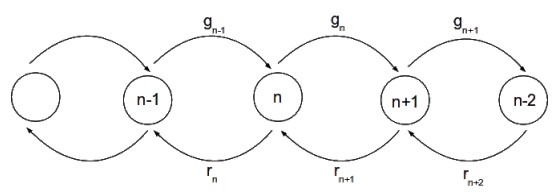
\includegraphics[scale=0.90]{theonestep.jpg}
\caption{ The one-step process with its transition probabilities and the different states. Image from \cite{Ragazza}.}
\label{theonestep}
\end{figure}
\newline 
Thus the master equation for one-step processes can be rewritten as
\begin{equation}\label{theonestepmasterequation}
\frac{dP_{n}(t)}{dt} = \dot{P_{n}} = r_{n+1}P_{n+1} + g_{n-1}P_{n-1}-(r_{n}+g_{n})P_{n}
\end{equation}
However, we need to beware to the boundary conditions. Given that we have a number of molecules \emph{n} that is $n \in [0,N]$, if $n = 0$ is a boundary, the Eq \ref{theonestepmasterequation} is meaningless and has to be replaced with 
\begin{equation}
\dot{P_{0}} = r_{1}P_{1} - g_{0}P_{0}
\end{equation}
since we need to set this condition $r_{0} = g_{-1} = 0$ otherwise we would have a negative number of molecules which is physically unfeasible. Similarly an upper boundary $n = N$ requires a special equation:
\begin{equation}
\dot{P_{N}} = g_{N-1}P_{N-1} - r_{N}P_{N}
\end{equation}
because the condition $r_{N+1}=g_{N}=0$ or then with $g_{N}$ we would have a transition from the state \emph{N} to the state $N+1$ and so to a state whose number of molecules is greater than the maximum number present in our system; a similar reasoning is done for $r_{N+1}$ that means a transition from the state $N+1$ to \emph{N}.


One-step processes can be subdivided based on the coefficients $r_{n}$ and $g_{n}$ into the following categories: linear, if the coefficients are linear functions of \emph{n}, nonlinear, if the coefficients are nonlinear functions of \emph{n} and random walks, if the coefficients are constant \cite{Ragazza,Math}.
\newline
An important example of a one-step process with constant transition probabilities is the \emph{Poisson process}, defined by
\begin{align}
    r_{n} = 0,g_{n}=q,p_{n}(0)=\delta_{n,0},
\end{align}
where \emph{q} is constant parameter. In such case, the master equation is
\begin{equation}
    \dot{P_{n}} = q(P_{n-1}-P_{n})
\end{equation}
The solution of this equation is a time dependent probability distribution
\begin{equation}
    P_{n}(t) = \frac{(qt)^{n}}{n!}e^{-qt}
\end{equation}
that is a Poisson distribution. Let us keep in mind this theoretical result for the discussion about modeling gene expression in Chapter \ref{models}.  

\section{Resolution Methods for the CME}

Solving the master equation would seem to be the ideal way of looking at stochastic systems, as it can tell us the full distribution of possible states the system can be in over time, but for one important disadvantage: its complexity. 

In some special cases it is possible to solve it with analytical and numerical methods, for instance in case of linearity of the process where every reaction term is constant or proportional to the first power of only one chemical specie \cite{PHD}.

However, in general, what makes it difficult to solve is the mixing of a continuous time evolution with a discrete evolution of the state variables \cite{SanDiegoUniversity}. Furthermore, this becomes apparent when considering how many equations must be solved at each time point, and bearing in mind that the number of possible states can increase exponentially with time \cite{Article}. 
 
Thus we must use trajectory-based approaches, which differ from the master equation in that they do not find the distribution of all possible states over time. Rather, \emph{they simulate single realizations}, meaning that at each step they choose one out of all the possible outcomes.

The trajectory of each stochastic simulation is different, since each is a single realisation sampled randomly from the full distribution given by the master equation. Given many of these random single trajectories, we can build up a picture of the full distribution.

Many approximation methods for the solution of the CME have been developed during the years and which operate by discretizing the time evolution. In this thesis, we will exploit the two simulation algorithms that have become the workhorse stochastic methods for many researchers today: the stochastic simulation algorithm (SSA) and the tau-leaping procedure. In the end, we will propose an ``alternative'' method that combines the two mentioned algorithms in order to speed up the stochastic simulation of a chemically reacting system. 

\subsection{Stochastic simulation algorithm (SSA)}
Most of the attempts in solving the CME have concentrated on Monte Carlo simulations using the \emph{stochastic simulation algorithm} (SSA) proposed by Gillespie in his seminal paper. This method is statistically exact, namely a full probability distribution built up from an infinite number of simulations will be identical to the distribution of the Markov process, given by the master equation \cite{Article}. This algorithm is arguably the simplest SSA variant and is based on the following steps in order to simulate \emph{one stochastic realisation}: assuming that the system is described by the state vector $\Vec{Y}$ which in general represents the amount of molecules for each chemical species and given that the initial state of the system is $\Vec{Y} = \Vec{Y}_{0}$, one has to choose which reaction happens between the possible ones and how much time the system will spend in such state before the next reaction happens \cite{PHD}. Each reaction \emph{i} is described by its \emph{transition rate} (or even called \emph{propensity}) $k_{i}$ and by the modification of the state vector that generate. Given that we are dealing with Markov process, the difference in time between two successive events $\Delta t$ follows an \emph{exponential distribution}, whose parameter is the propensity $k_{i}$:
\begin{equation}
    p_{i}(\Delta t) = e^{-k_{i}\Delta t}
\end{equation}
given that any reaction is independent from the others, the distance in time between two successive events is distributed as:
\begin{equation}\label{exponential}
    p(\Delta t) = e^{-\sum_{i=0}^{R} k_{i} \Delta t}
\end{equation}
This process is iterated untill the whole time of interest has been simulated or untill an other desired condition is achieved.


Unfortunately, the direct method SSA pays the price for its simplicity in computational time, as two random numbers must be generated at each step \cite{Article} (the one for choice of the event and the other for the choice of the time spent in the state given by an exponential random variable). Furthermore, the SSA has an inherent limitation: it must simulate every single reaction. This is, of course, its great strength too, but in cases where there are many reactions or larger molecular populations, it often becomes too slow to generate useful numbers of simulations in a practical time period.

\subsection{Tau-leap algorithm}
The tau-leap method, or also referred as explicit tau-leaping procedure, is similar to the SSA in that each simulation is a \emph{single stochastic realisation} from the full distribution at each step \cite{Article}. However, the steps are fixed  and in each one of these \emph{it counts the total number of occurrences of each type of reaction over that step approximating the number of firings of each reaction channel during a chosen time increment $\tau$ as a Poisson random variable}. Thus, also in this case based on the initial state of molecular populations $\Vec{Y}=\Vec{Y_{0}}$, if there are \emph{M} reactions, we take \emph{M} Poisson random number samples. We can call the time interval in which these reactions happen as $\tau$. Hence, the vector of molecules given by the \emph{M} reactions $\Vec{Y}=\Vec{Y}_{M}$ in the time interval $\tau$ is given by
\begin{equation}\label{MPoissonReactions}
    \Vec{Y}_{m}(\tau) = P(\Vec{K_{i}}\tau)
\end{equation}
where \emph{P} is the Poisson distribution with mean equal to $\Vec{K_{i}}\tau$ of which $\Vec{K_{i}}$ is the vector of propensities. Then the initial state of molecular populations is updated based on Eq \ref{MPoissonReactions}  and this is iterated untill the whole time of interest has been simulated or a desired condition is met, similarly to SSA.


Hence, the basic idea of this procedure is to advance the system by a \emph{pre-selected} time increment $\tau$ (in contrast to the generated time increment that is in the SSA), which is large enough that many reaction events occur in that time, but nevertheless small enough that \emph{no propensity function value is likely to change ``significantly'' as a consequence of those reaction events} \cite{Method}.


Summing all up, tau-leap algorithm has the key advantage that we now do not need to spend time simulating individual reactions and as such it is much faster than the SSA. On the other hand its main drawback is that we have lost accuracy compared to the SSA in some ways such as we do not know when each reaction occurred within the time step.
% how many reactions occurred (we can only estimate this)


The accuracy issue can be mitigated (at the expense of computational time) as the error level, and so time step size, is decreased; indeed, as the time step tends to zero, the tau-leap effectively becomes the SSA, with each step experiencing either zero or one reaction \cite{Article}. 


Moreover, as anticipated in some rows above, there is another complementary issue with the tau-leap: as many reactions are simulated at once, molecular species that are depleted in any reaction can go negative if the time step is too large. This is obviously unphysical, and so undesirable and makes it inappropriate to simulate reactions that regards species which are typically lower in number such as genes. 

Fig. \ref{ODESSATAULEAP} shows the number of RNA molecules and proteins produced during time obtained by using the just explained stochastic simulation methods (SSA and Tau-leap) and those given by the deterministic approach, i.e. ordinary differential equation solution, considering a model with a gene that is always expressed (see section \ref{modelconstitutivegeneexpression}). In this particular case in which the RNA production rate is higher than the degradation rate and the same is for proteins, we do not run the risk to obtain unphysical negative number of molecules and we can compare the results given by the algorithms. In particular, we consider the following values of rates: gene activation $k_{a}=1$, gene deactivation $k_{i}=0$, RNA production $k_{1}=1$, RNA degradation $k_{2}=0.1$, protein production $k_{3}=1$, protein degradation $k_{4}=0.1$.

\begin{figure}[!ht]
\centering
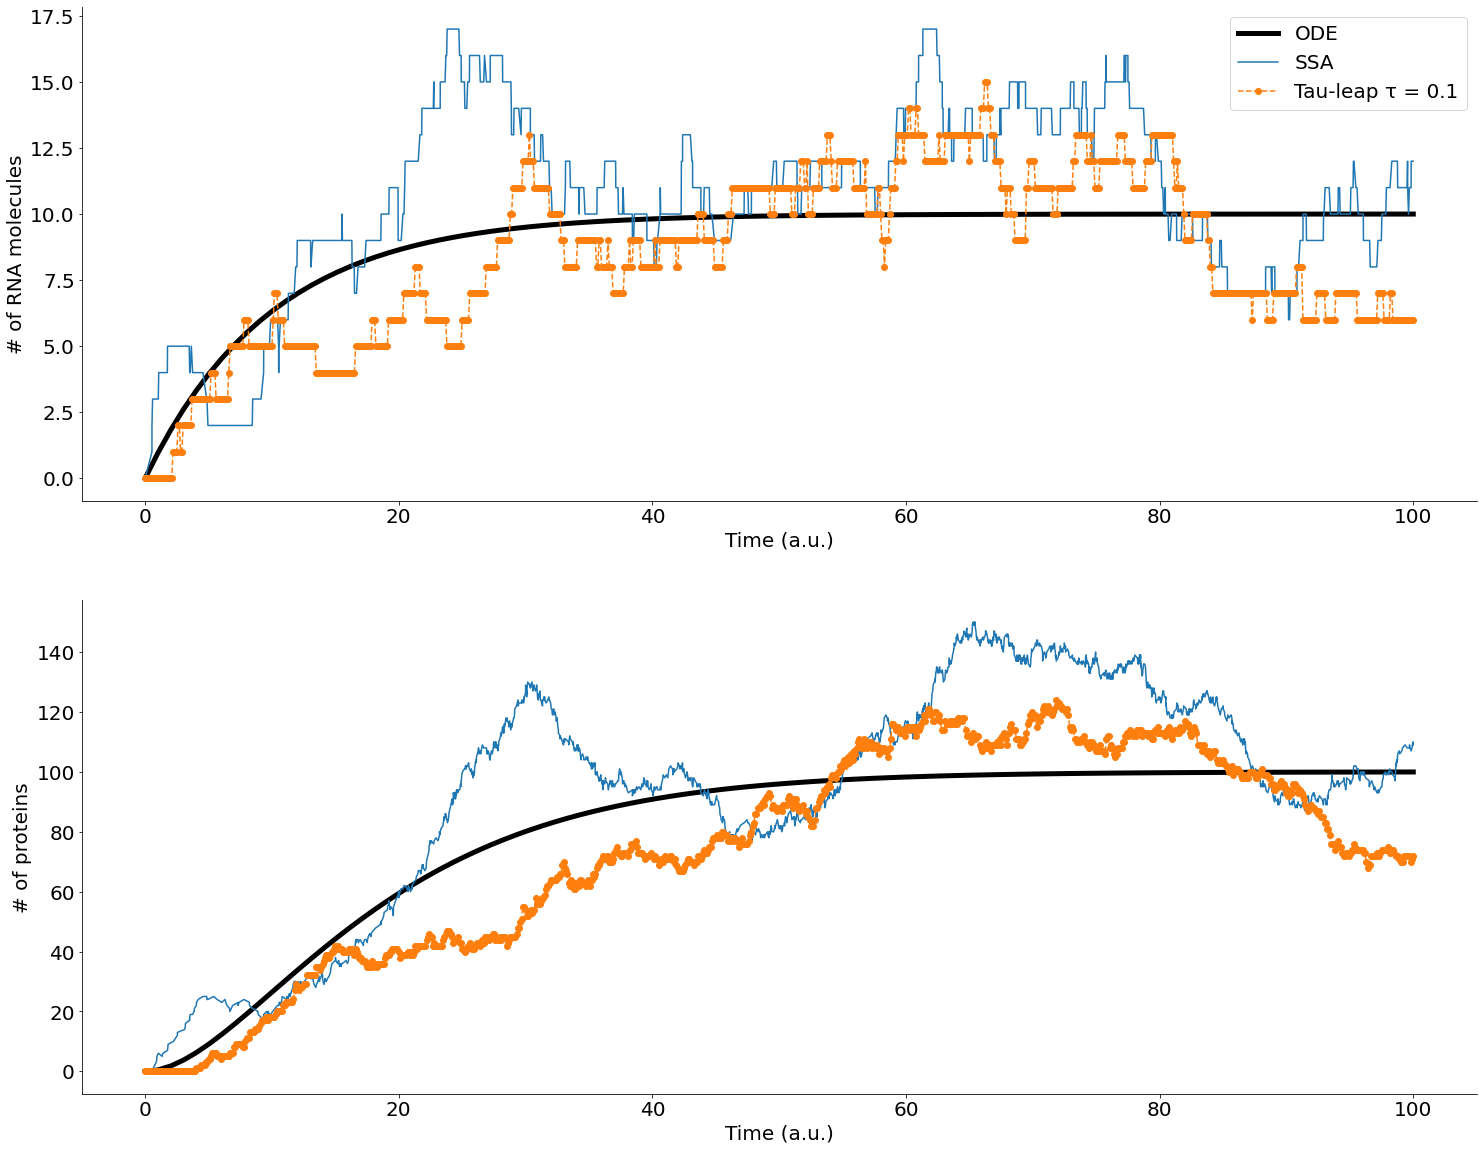
\includegraphics[scale=0.30]{ODESSATauleaptimeplot100au.png}
\caption{Comparison of simulation methods. The typical trajectory of the number of molecules as function of time is reported from the SSA (blue line) and tau-leap (orange dotted line) and ODE solution (black thick line). The upper plot refers to the number of RNAs molecules produced as a function of time starting from a gene that is always active, while the plot below represents the number of proteins produced starting from the RNAs of the same model.}
\label{ODESSATAULEAP}
\end{figure}

From Fig. \ref{ODESSATAULEAP}, we notice that trends resulting from the three methods are similar both for the number of RNA molecules and for the number of proteins produced during time. 

However, in order to compare the two stochastic simulation methods, it is more useful to compare the stationary distributions (i.e. the distribution of states) obtained instead of the time dependent results. 

Hence, we run the same simulation till a longer time limit to allow to obtain the expected Poisson distributions. The results are shown in Fig. \ref{SSATauleapdistribution}:

\begin{figure}[!ht]
\centering
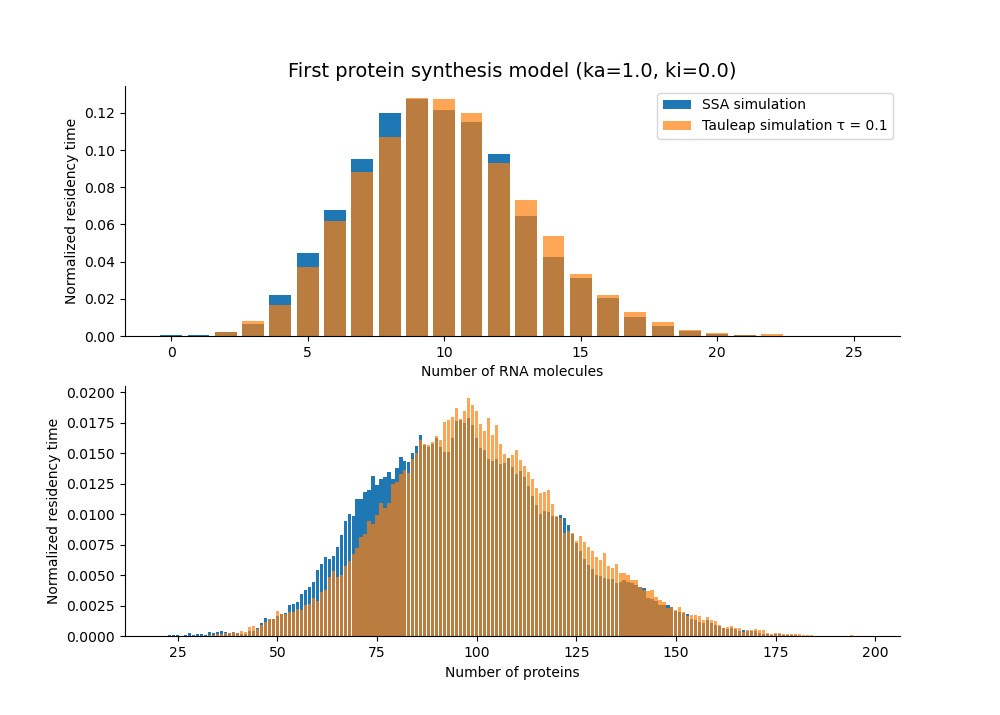
\includegraphics[scale=0.70]{RemovingwarmupSSA55.25sTauleap10.22stimelimit9000.png}
\caption{Comparison of simulation methods by using the stationary distributions given by the SSA (orange bar plot) and tau-leap (blue bar plot).}
\label{SSATauleapdistribution}
\end{figure}
\newpage
There is a clear overlap between the two distributions, showing that the SSA simulation is providing the same results to the Tauleaping, validating also that the two algorithms work in representing the stochastic trajectory of the chemical reacting system we are analysing.

The time plot referred to the stationary distribution shown in Fig. \ref{SSATauleapdistribution} is the one reported in Fig. \ref{ODESSATauleaptimeplot9000}: 

\begin{figure}[!ht]
\centering
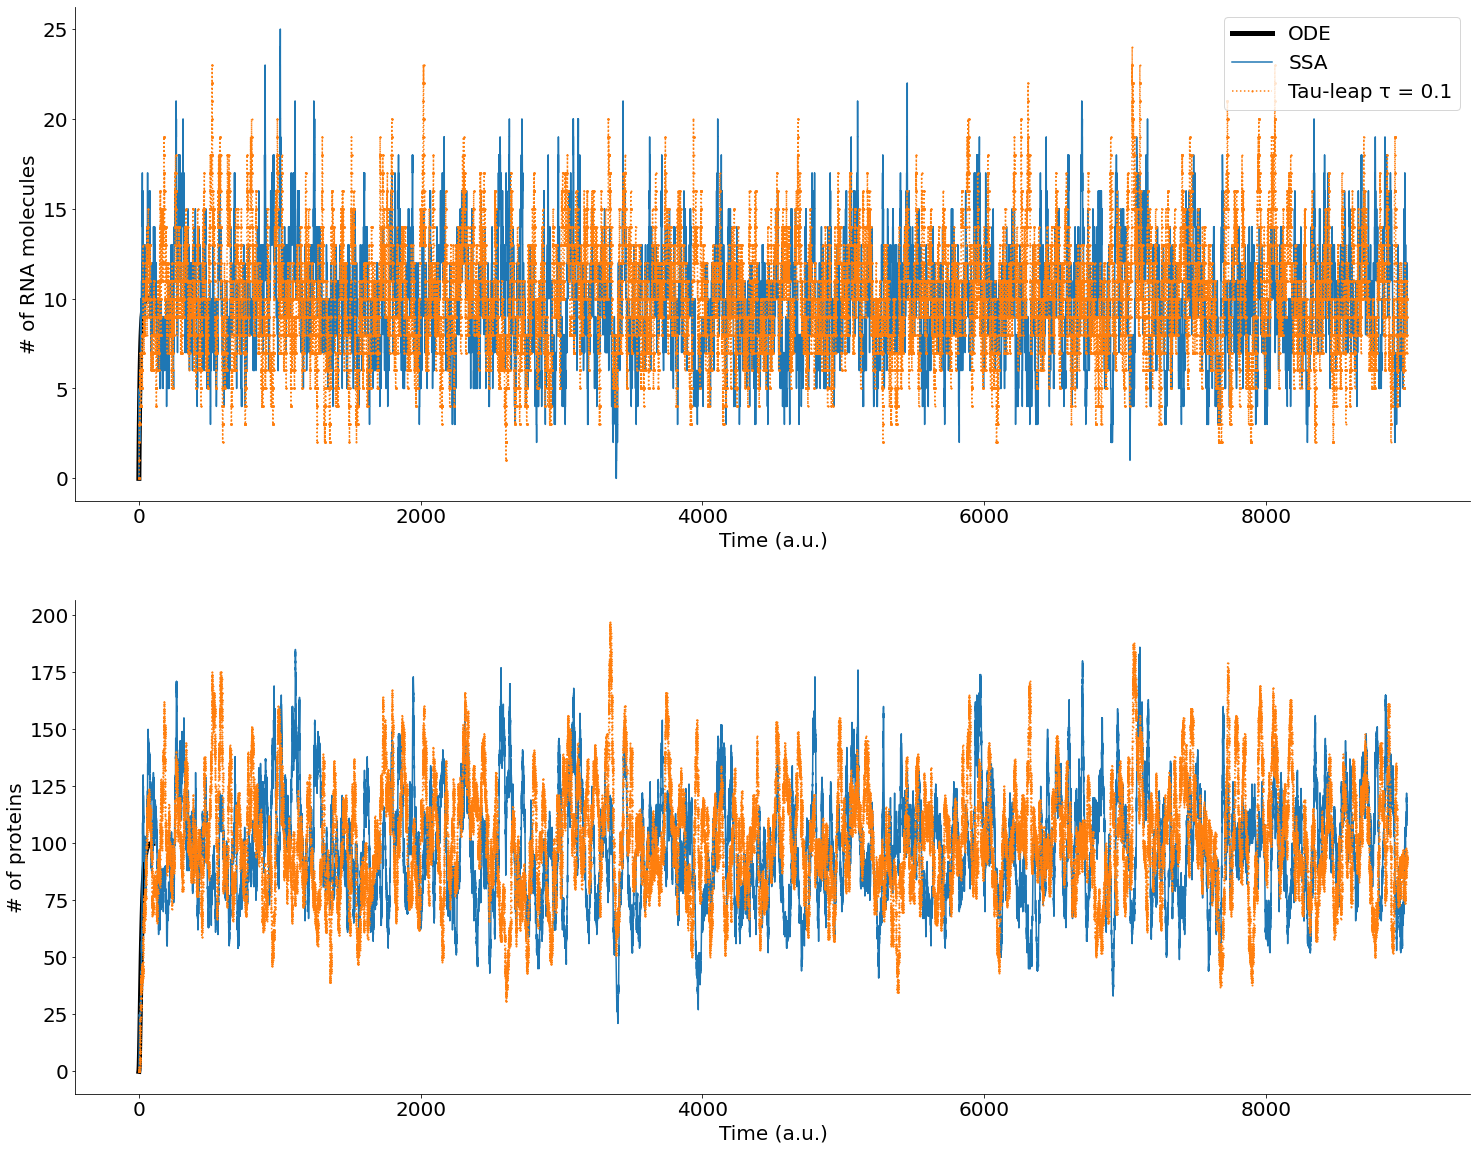
\includegraphics[scale=0.30]{ODESSATauleaptimeplot9000au.png}
\caption{Comparison of simulation methods using a higher time limit than the one in Fig.\ref{ODESSATAULEAP}. The typical trajectory of the number of molecules as function of time is reported from the SSA (blue line) and tau-leap (orange dotted line) and ODE solution (black thick line).}
\label{ODESSATauleaptimeplot9000}
\end{figure}
\newpage
%I parametri del modello erano ka=1, ki=0, k1=1, k2=0.1, k3=0.1, k4=1, k5=0.001, time limit 100.
Also in Fig. \ref{ODESSATauleaptimeplot9000}, the ODE solution is reported. We can notice that the deterministic approach, even though cannot be considered representative of the true behaviour of the system, its result represent a useful statistic of the system that in this case is the means of our unimodal symmetric distributions of the number of RNAs and proteins produced. The black line in Fig. \ref{ODESSATAULEAP} and \ref{ODESSATauleaptimeplot9000} is in fact a rolling mean of the stochastic simulation.

Furthermore, deterministic simulations are generally much faster to run than their statistical counterparts \cite{Article}.

In order to make this simulation for a virtual time equal to 9000 with a computer of 1.10 GHz CPU, the SSA simulation has spent 55 seconds with respect to the 10 seconds spent by the explicit tau-leaping algorithm. 

However the tau-leaping algorithm can work well in this situation of constitutive gene expression. And what if our gene is regulated ? The risk of running in negative number of molecules is much higher hence we need an algorithm that checks that this does not occur if we want to go on using the tau-leap procedure.

In this kind of system, the typical choice is to combine the SSA and the tau-leaping procedure because the first one can simulate the gene behavior while the second one is suitable for simulating the changing of more numerous molecular species such as RNAs and proteins.

In the next section, we propose and describe a combined SSA/tau-leaping algorithm.

\subsection{An alternative method: the ``hybrid''stochastic simulation algorithm}

%METTICI PI� FORMULE PER DESCRIVERE OGNI STEP. Inoltre specifica che questi metodi servono sia per cercare un modo per velocizzare la simulazione (cosa che � molto importante) per� anche per attestare che i risultati che otteniamo sono giusti ossia che i metodi funzionano. Dunque bisogna controllare le autocorrelazioni dei diversi metodi con le incertezze e verificare che sono uguali.+ Nota che la configurazione dell'autorepressore � il peggio che possiamo chiedere al Tau-leap e l'efficienza di questi metodi (ossia il tempo impiegato per fare la simulazione) appunto dipende molto dalla configurazione che stiamo considerando.



Many schemes have been developed that allow the choice of larger time steps in the Tau-leap algorithm whilst avoiding negative populations. In this thesis work, we have tried an approach that combines, basically, the SSA with Tau-leap algorithm in a way that the first one updates the state of genes while the latter updates the state of other more numerous species such as RNA molecules and proteins.

The model that we consider to develop this ``hybrid'' algorithm is the first simple protein synthesis model (we will describe in more details the basic genetic models in Chapter \ref{models}). We have 3 molecular species: one \emph{gene} whose transcription leads to \emph{RNAs} production that are translated into \emph{proteins}. In other words, this is what is called as \emph{the central dogma of biology}, that states that genes specify the sequence of mRNA molecules, which in turn specify the sequence of proteins (DNA $\rightarrow$ RNA $\rightarrow$ Protein).

Hence we have 6 possible reactions: gene activation, gene deactivation, RNA production, RNA degradation, protein production and protein degradation.

Let us consider our usual state of molecular populations $\Vec{Y}$ and the initial state $\Vec{Y}=\Vec{Y_{0}}$. The transition rates related to such state is $\Vec{K}=\Vec{K}_{0}$.
%\Vec{\mathbf{K}}=\Vec{\mathbf{K_{0}}}

The proposed hybrid algorithm is based on the following steps:
\begin{enumerate}
 \item In state $\Vec{Y}$ at time \emph{t}, evaluate the transitions rates of all species and those related to genes $\Vec{K}_{genes}$.
 \item Apply the SSA algorithm by considering the sum of genes transition rates in Eq.\ref{exponential} and hence select the reactions that modify the time of residency of the gene state. 
 \item Eq.\ref{exponential} represents in this case the time of residency of the gene $t_{gene\_state\_residency}$ in the initial state. The aim of this algorithm is to speed up the SSA by considering such $t_{gene\_state\_residency}$ as the tau $\tau$ in the Tauleaping.
 \item Thus, after the SSA application, consider the $t_{gene\_state\_residency}$ and the updated gene state $\Vec{Y}'$.
 \item Apply the Tauleaping algorithm to the RNAs and proteins state and by considering $t_{gene\_state\_residency}$ as $\tau$, so $t_{gene\_state\_residency} = \tau$ .
 
 \item Consider the updated state by the tauleaping and SSA $\Vec{Y}'$ and compute also the difference between the transition rates $\Vec{K}_{0}$ refered to the initial state $\Vec{Y}_{0}$ and the final value of transition rate $\Vec{K}'$ obtained considering the updated state $\Vec{Y}'$. In particular compute the following difference:
 \begin{equation}
  \Delta \Vec{K} = \left|\frac{\Vec{K}'}{K'_{TOT}}-\frac{\Vec{K}}{K_{TOT}}\right|
 \end{equation}
where $K'_{TOT}$ is the sum of all the transition rates calculated with the new updated state $\Vec{Y}'$ and the same for $K_{TOT}$ that is the sum of all the transition rates calculated with the initial state $\Vec{Y}_{0}$.

Let us rember indeed that we are dealing with first order kinetics reactions, whose transition rates are propotional to the amount of molecules of interest by a constant $k$.

$\Vec{Y}'$ and $\Delta \Vec{K}$ are the two quantities that must be monitored, because, as regards the first one, of course, we need to check that there are not negative number of molecules; for the latter, if it is too large, it can lead in very low accuracy in the algorithm results. For instance, if there is a tauleaping step that leads to a final state $\Vec{Y}'$ that has a much higher number of proteins with respect to the initial state $\Vec{Y}_{0}$, the final stationary distribution will result in an ``explosion'' in the number of molecules that does not represent the true distribution. 

Thus, in the following steps we describe how we monitor these two quantities.

\item If $\Vec{Y}'$ has all positive values and $\Delta \Vec{K}$ is lower than a given threashold chosen by the user, update rates and the state by considering the results of the SSA and tauleaping algorithms already applied in points 2 and 5. If the simulation is running untill a precise time limit (as we always do in this thesis work), update the time of observation using the $t_{gene\_state\_residency}$. 

\item If instead $\Vec{Y}'$ has a negative number of molecules or one of $\Delta \Vec{K}$ is higher than the threashold, it means that we need to make smaller steps than the one proposed by the SSA.

Hence we divide by one half $\tau$, $\tau' \rightarrow \tau/2$, untill the conditions on the number of molecules and on the $\Delta \Vec{K}$ are satisfied.

When we obtain the right $\tau'$, we use it to make a tauleaping, updating the RNAs and proteins states.

Then, we attempt a tauleaping using the remaining time $\tau - \tau'$ that we call as $\tau''$.

If the conditions are satisfied, we update the total time of observation with $\tau$ and attempt a new tau-leaping starting from point 1 by considering a new updated state $\Vec{Y}'$ and the new rates $\Vec{K}'$.

If it is not, we divide again $\tau''$ by one half, $\tau''' \rightarrow \tau''/2$ untill the desired conditions are met.

This process is iterated untill the $\tau^{(n)}$ is higher than 3 times the characteristic time $t_{c}$ given by the SSA by considering all reactions happening in our system.

\item If the new $\tau^{(n)}$ reaches a lower value, i.e. $\tau^{(n)} \leq 3t_{c}$, it is worth to make a SSA step without getting trapped in the previous iterating system that is certainly less precise than the SSA. In this case, update the total time with the characteristic time given by the SSA applied considering all the reactions that are possible in our system.

\item Apply steps from 1 to 9 untill the desired total time is reached or the desired condition is met.
\end{enumerate}

As in the tauleaping section, we have compared the results of the new algorithm stationary distribution with the SSA. We consider the following model parameters: activation rate $k_{a}=1$, deactivation rate $k_{i}=0.5$, RNA production rate $k_{1}=1$, RNA degradation rate $k_{2}=0.1$, protein production rate $k_{3}=1$, protein degradation rate $k_{4}=0.1$. These are the same parameters and the same model used to compare the SSA simulation with the tauleaping simulation except for the fact that the deactivation rate is now different from 0. Indeed now we can simulate without worrying about the fact that the number of molecules becomes negative and so we can add gene regulation to our model.

We consider a threashold $\Delta K_{t} = 10$ and the result for our basic model is promising.
\newpage
\begin{figure}[!ht]
\centering
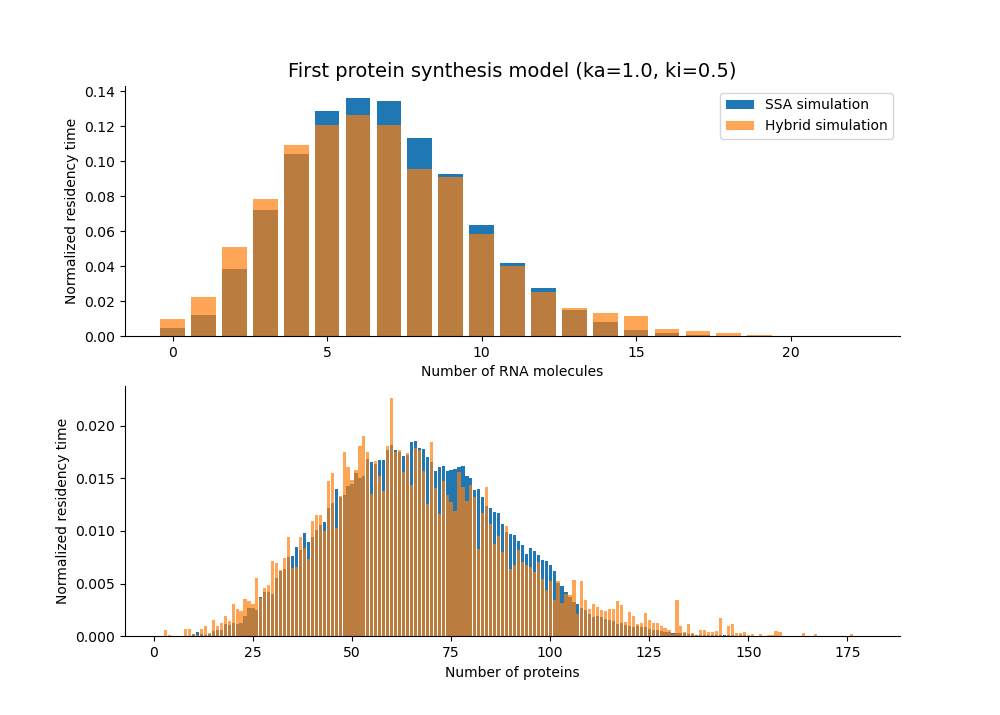
\includegraphics[scale=0.70]{ka1ki0.5SSA1min47sHybrid7.5stimelimit14000.png}
\caption{Comparison of simulation methods using stationary distributions. The blue bar plot is the result given by the SSA algorithm while the orange bar plot is the result given by the hybrid algorithm.}
\label{SSAHybridBasicModel}
\end{figure}

Fig. \ref{SSAHybridBasicModel} shows the distribution of states given by the SSA (blue bar plot) and the hybrid algorithm (orange bar plot). They show a high degree of overlapping with hybrid approach speed that is about 10 times lower than the SSA. More precisely, using a computer with 1.10 GHz, the speed results are summed up in the table \ref{tablebasicmodel}.

\begin{table}[!h]
\begin{center}
\begin{tabular}{ |c|c|c| } 
 \hline
       & \textbf{speed} \\
 \hline
 SSA & 107s \\
 \hline
 Hybrid & 7.5s \\ 
 \hline
\end{tabular}
\caption{\label{tablebasicmodel}Computational time required for the SSA and Hybrid algorithm in case of our basic model.}
\end{center}
\end{table}
\newpage

We can modify the model changing the parameter value $k_{1}$ (that in the end it is also at the basis of the distribution). By considering $k_{1}=10$, the related stationary distribution is shown in Fig. \ref{SSAHybridk110}.   

\begin{figure}[!ht]
\centering
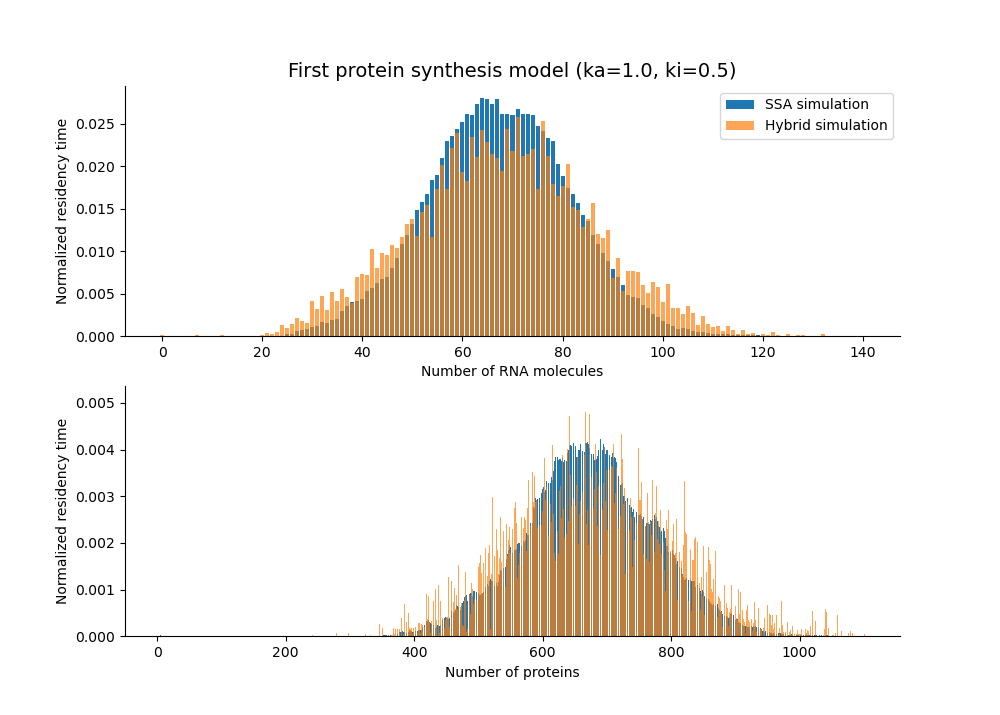
\includegraphics[scale=0.70]{ka1ki0.5SSA11min58sHybrid7.7stimelimit14000k110.png}
\caption{Comparison of simulation methods using stationary distributions with $k_{1}=10$. The blue bar plot is the result given by the SSA algorithm while the orange bar plot is the result given by the hybrid algorithm.}
\label{SSAHybridk110}
\end{figure}
\newpage
There is still a high degree of overlap between the two distributions even though the protein hybrid distribution result is more scattered with respect to the SSA. In this case, the gain in velocity is really high. Once again, the relative speeds are reported in the table \ref{tablek110}.

\begin{table}[!h]
\begin{center}
\begin{tabular}{ |c|c|c| } 
 \hline
       & \textbf{speed} \\
 \hline
 SSA & 718s \\
 \hline
 Hybrid & 8s \\ 
 \hline
\end{tabular}
\caption{\label{tablek110}Computational time required for the SSA and Hybrid algorithm is case $k_{1}=10$.}
\end{center}
\end{table}


However, the situation changes if we decrease 10 times the rate of RNA production and so $k1=0.1$ instead of increasing it by 10 times as in the previous case.

\begin{figure}[!ht]
\centering
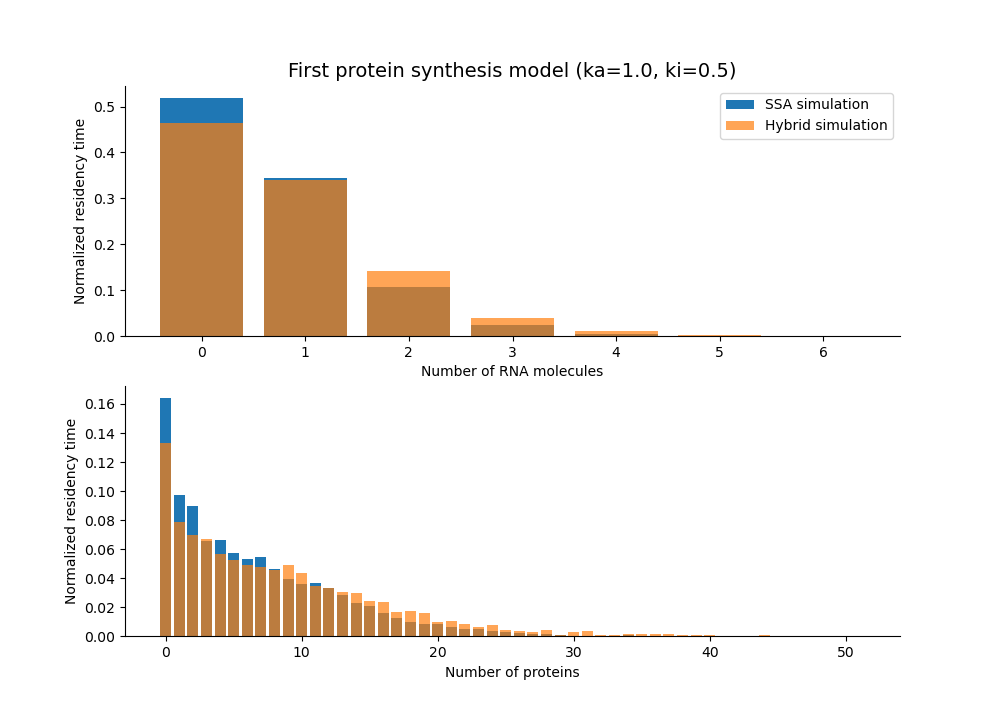
\includegraphics[scale=0.70]{ka1ki0.5SSA8.31sHybrid7.9stimelimit14000k10.1.png}
\caption{Comparison of simulation methods using stationary distributions with $k_{1}=0.1$. The blue bar plot is the result given by the SSA algorithm while the orange bar plot is the result given by the hybrid algorithm.}
\label{SSAHybridk10.1}
\end{figure}
\newpage
The degree of overlap is still high, however we do not achieve a considerable improvement in velocity:

\begin{table}[!h]
\begin{center}
\begin{tabular}{ |c|c|c| } 
 \hline
       & \textbf{speed} \\
 \hline
 SSA & 8.3s \\
 \hline
 Hybrid & 7.9s \\ 
 \hline
\end{tabular}
\caption{\label{tablek10.1}Computational time required for the SSA and Hybrid algorithm is case $k_{1}=0.1$.}
\end{center}
\end{table}

This suggests that decreasing the number of RNAs produced, the performance of our hybrid algorithm decreases. What if we consider the opposite type of regulation ? 

Let us consider $k_{a}=0.1$ and $k_{i}=1$ and let the other parameters equal to the basic model values.

\begin{figure}[!ht]
\centering
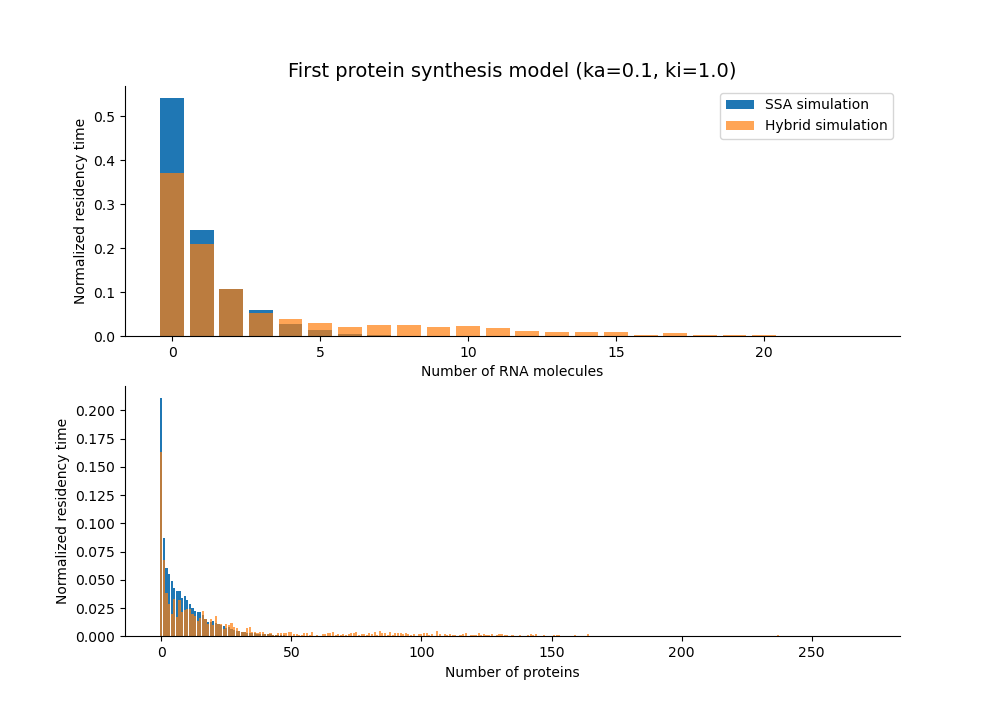
\includegraphics[scale=0.70]{ka0.1ki1SSA9sHybrid35stimelimit14000.png}
\caption{Comparison of simulation methods using stationary distributions considering gene activation rate lower than the deactivation rate ($k_{a}=0.1$ and $k_{i}=1$). The blue bar plot is the result given by the SSA algorithm while the orange bar plot is the result given by the hybrid algorithm.}
\label{SSAHybridka0.1ki1}
\end{figure}

Fig. \ref{SSAHybridka0.1ki1} shows the effects of this other kind of regulation on the distribution given by the two algorithms. As expected, in both cases the results show that the residency time refered to the state with the number of molecules equal to zero is the highest. However, in this case, the hybrid algorithm shows an increase in the number of molecules state both in the RNAs and even more in the proteins states. One can try to decrease the threashold $\Delta K_{t}$ but at expence of computational time that is already 3 times higher than the SSA (see table \ref{ka0.1ki1}).

\begin{table}
\begin{center}
\begin{tabular}{ |c|c|c| } 
 \hline
       & \textbf{speed} \\
 \hline
 SSA & 9s \\
 \hline
 Hybrid & 35s \\ 
 \hline
\end{tabular}
\caption{\label{ka0.1ki1}Computational time required for the SSA and Hybrid algorithm is case $k_{a}=0.1$ and $k_{i}=1$.}
\end{center}
\end{table}

Hence we can conclude that this proposed hybrid algorithm works very well from the point of view of accuracy and computational time when the model tends to produce a high number of molecules, whereas we still do not find an approach that is better than Gillespie's algorithm when the number of molecules produced is low. Anyway, in such cases of low number of molecules, the SSA is efficient and there is not a huge needing to be optimized.%E' meno efficiente in questi casi perch� tendiamo ad andare negli altri if.

Furthemore, we need to notice that our algorithm is a ``paramater-dependent'' algorithm, where the parameter is $\Delta k_{t}$. As regards how tuning this parameter, we can suggest to keep its value as high as possible if one wants to increase the speed but paying attention to the accuracy because with an higher $\Delta k_{t}$ you will run the risk of ``the explosion of molecules''. 

One can notice, indeed, that the logic of our hybrid algorithm is similar to the Adaptive Runge-Kutta methods used for the approximate solutions of simultaneous nonlinear equations: during the integration, the step size is adapted such that the estimated error stays below a user-defined threshold. If the error is too high, a step is repeated with a lower step size; if the error is much smaller, the step size is increased to save time \cite{RungeKutta}.

Anyway, in this thesis work we will use the Stochastic Simulation Algorithm because our hybrid approach needs to be further tested and improved.



%L'algoritmo sembra funzionare meglio quando c'� una maggiore produzione di molecole (controlla proprio cosa succede: quante volte andiamo a finire in un if e quante in un altro).

%The trends of molecules vs time of these methods in this case are almost overlapping, as seen by eye. However, we can make a more quantitative comparison of these different approaches by computing the means of different simulations and the relative standard deviations.
%autocorrelation con k4 0.01 e relativi plot nel tempo.
%quantili

%DOMANDA AL PROFESSORE: We need to point out, anyway, that the efficiency of these algorithms, i.e. the simulation execution times, depend on the biological model that we are considering. In the next part we will discuss about some important biological models. For the moment, we can say that, for example, the pure SSA algorithm is still efficient for systems where the number of species keeps low as for the case of \emph{autorepressor} where there is only one gene and the proteins produced by their ``father'' gene reduces the probability of activation of the same gene.     



\section{Statistical analysis techniques for warm-up detection}
Up to now we have shown the results of stationary distributions of the CME for comparing different algorithms. However we have omitted to explain an important analysis step when dealing with simulations: the warm-up detection and its removal. 

We can define our simulations as  ``infinite horizon simulations'': it has no natural beginning point or ending point. The desired starting conditions are sometimes in the far off future. We are interested in the long-run performance of the system and since there is no natural ending point of interest, we consider the horizon infinite \cite{Manuel}.  

As mentioned in section \ref{ACFSubsection}, sometimes we are interested in finding the moments of the probability distributions, such as the mean.

It is true that if the steady state distribution exists and you run the simulation long enough the estimators will tend to converge to the desired quantities. You can observe it in plots reported in Fig. \ref{ODESSATAULEAP} and \ref{SSATauleapdistribution}. At the beginning the number of molecules is low. Then by increasing virtual time, they increase untill they reach a state that we can call as ``steady'' state, that means that the distribution of the desired performance measure has reached a point where it is sufficiently similar to the desired steady state distribution \cite{Manuel}. 

We have also mentioned in section \ref{TheCMESection}, when talking about Chemical Master Equation solutions, that the eigenvector called also as the metastable state is the longest-standing one and its eigenvalue gives a time-scale of the time of convergence to the stationary distribution.

We need to clarify that ``steady state'' is a concept involving the performance measures generated by the system as time goes to infinity. It does not mean that the system itself has reached steady state.

The system never reaches steady state. If the system itself reached steady state, then by implication it would never change with respect to time. The system continues to evolve with respect to time.

The period before the so called steady state can affect the mean calculation and so also the distribution of states. This period is called warmup-period.

At the end of the warm up period, the system can be in any of the possible states of the system. Some states will be more likely than others.

Thus, within the infinite horizon simulation context, you must decide on how long to run the simulations and how to handle the effect of \emph{the initial conditions} on the estimates of performance by estimating when the warmup period ends, i.e. a time point that we can indicate also with $T_{w}$.   

The initial conditions of a simulation represent the state of the system when the simulation is started.

If $T_{w}$ is long enough, then on average across the replications, you are more likely to start collecting data when the system in states that are more representative over long term (rather than just states with low number of molecules).



\subsection{The effect of initial conditions}
Consider the output stochastic process $Y_{i}$ of the simulation and let $F_{i}(y|I)$ be the conditional cumulative distribution function of $Y_{i}$ where \emph{I} represents the initial conditions used to start the simulation at time 0.  If $F_{i}(y|I) \rightarrow F(y)$ when $i \rightarrow \infty$ for all conditions \emph{I}, then $F(y)$ is called the steady state distribution of the output process.

The distribution $F_{i}(y|I)$ at the start of the simulation, however, tends to depend more heavily upon the initial conditions. Estimators of steady state performance, such as the sample average, will tend to be biased.

If the expected value of the sampling distribution is equal to the parameter of interest then the estimator is said to be unbiased, i.e. $E[\hat{\theta}] = \theta $, with $\hat{\theta}$ a point estimator.

If instead the estimator is biased then the difference $E[\hat{\theta}] - \theta \neq 0$ and this difference is the bias of the estimator $\hat{\theta}$.

This is the so called initialization bias problem in steady state simulation or warm up problem. The warm-up period $d$ is the period such that given $Y_{i}$ with $i=d+1,...$, $Y_{i}$ \emph{will have substantially similar distributional properties as the steady state distribution}.


Unless the initial conditions of the simulation can be generated according to $F(y)$, which is not known, you must focus on methods that detect and/or mitigate the presence of initialization bias.












%Metti il dogma centrale della biologia. Si tratta di un sistema stiff con le proteine che si producono pi� velocemente perch� ad ogni RNA corrisponde una proteina o pi� proteine ? Mentre invece da un solo singolo gene partono pi� molecole di RNA. Infatti il tempo di warm up nel caso delle proteine � maggiore del caso dell'RNA che raggiunge uno stato stazionario che ha una media minore. 
%Sito.
%Immagine del periodo di warmup.

\subsection{``Replication-deletion'' method}
There are many methods that aim to determine the warmup period. In this thesis work we have used the a strategy that we can call ``replication-deletion'' method because it is based on the following steps:
\begin{enumerate}
 \item Make \emph{R} replications. Typically $R \geq 5$ is recommended.
 \item Since the sample points in SSA are obtained at different time intervals for each simulation, we interpolate them at constant intervals (we choose $dt=0.01$).
 \item Thank to the previous step, we can make the average across the replications. 
 
 Let $Y_{rj}$ be the $j^{th}$ observation on replication \emph{r} $j=1,2,...,m$ where \emph{m} is the minimum of the number of observations in the $r^{th}$ replication, $m=min(m_{r})$.
 
 \begin{equation}
  \hat{Y}=\sum_{r=1}^{n} Y_{rj}
 \end{equation}
 
 \item Find $T_{w}$ in $\hat{Y}$ by calculating the difference between $\hat{Y}$ at t and at t+dt, t+dt and t+2dt etc... when the differences start to become constant, then t is $T_{w}$ that we are looking for.

\end{enumerate}

\begin{figure}[!ht]
\centering
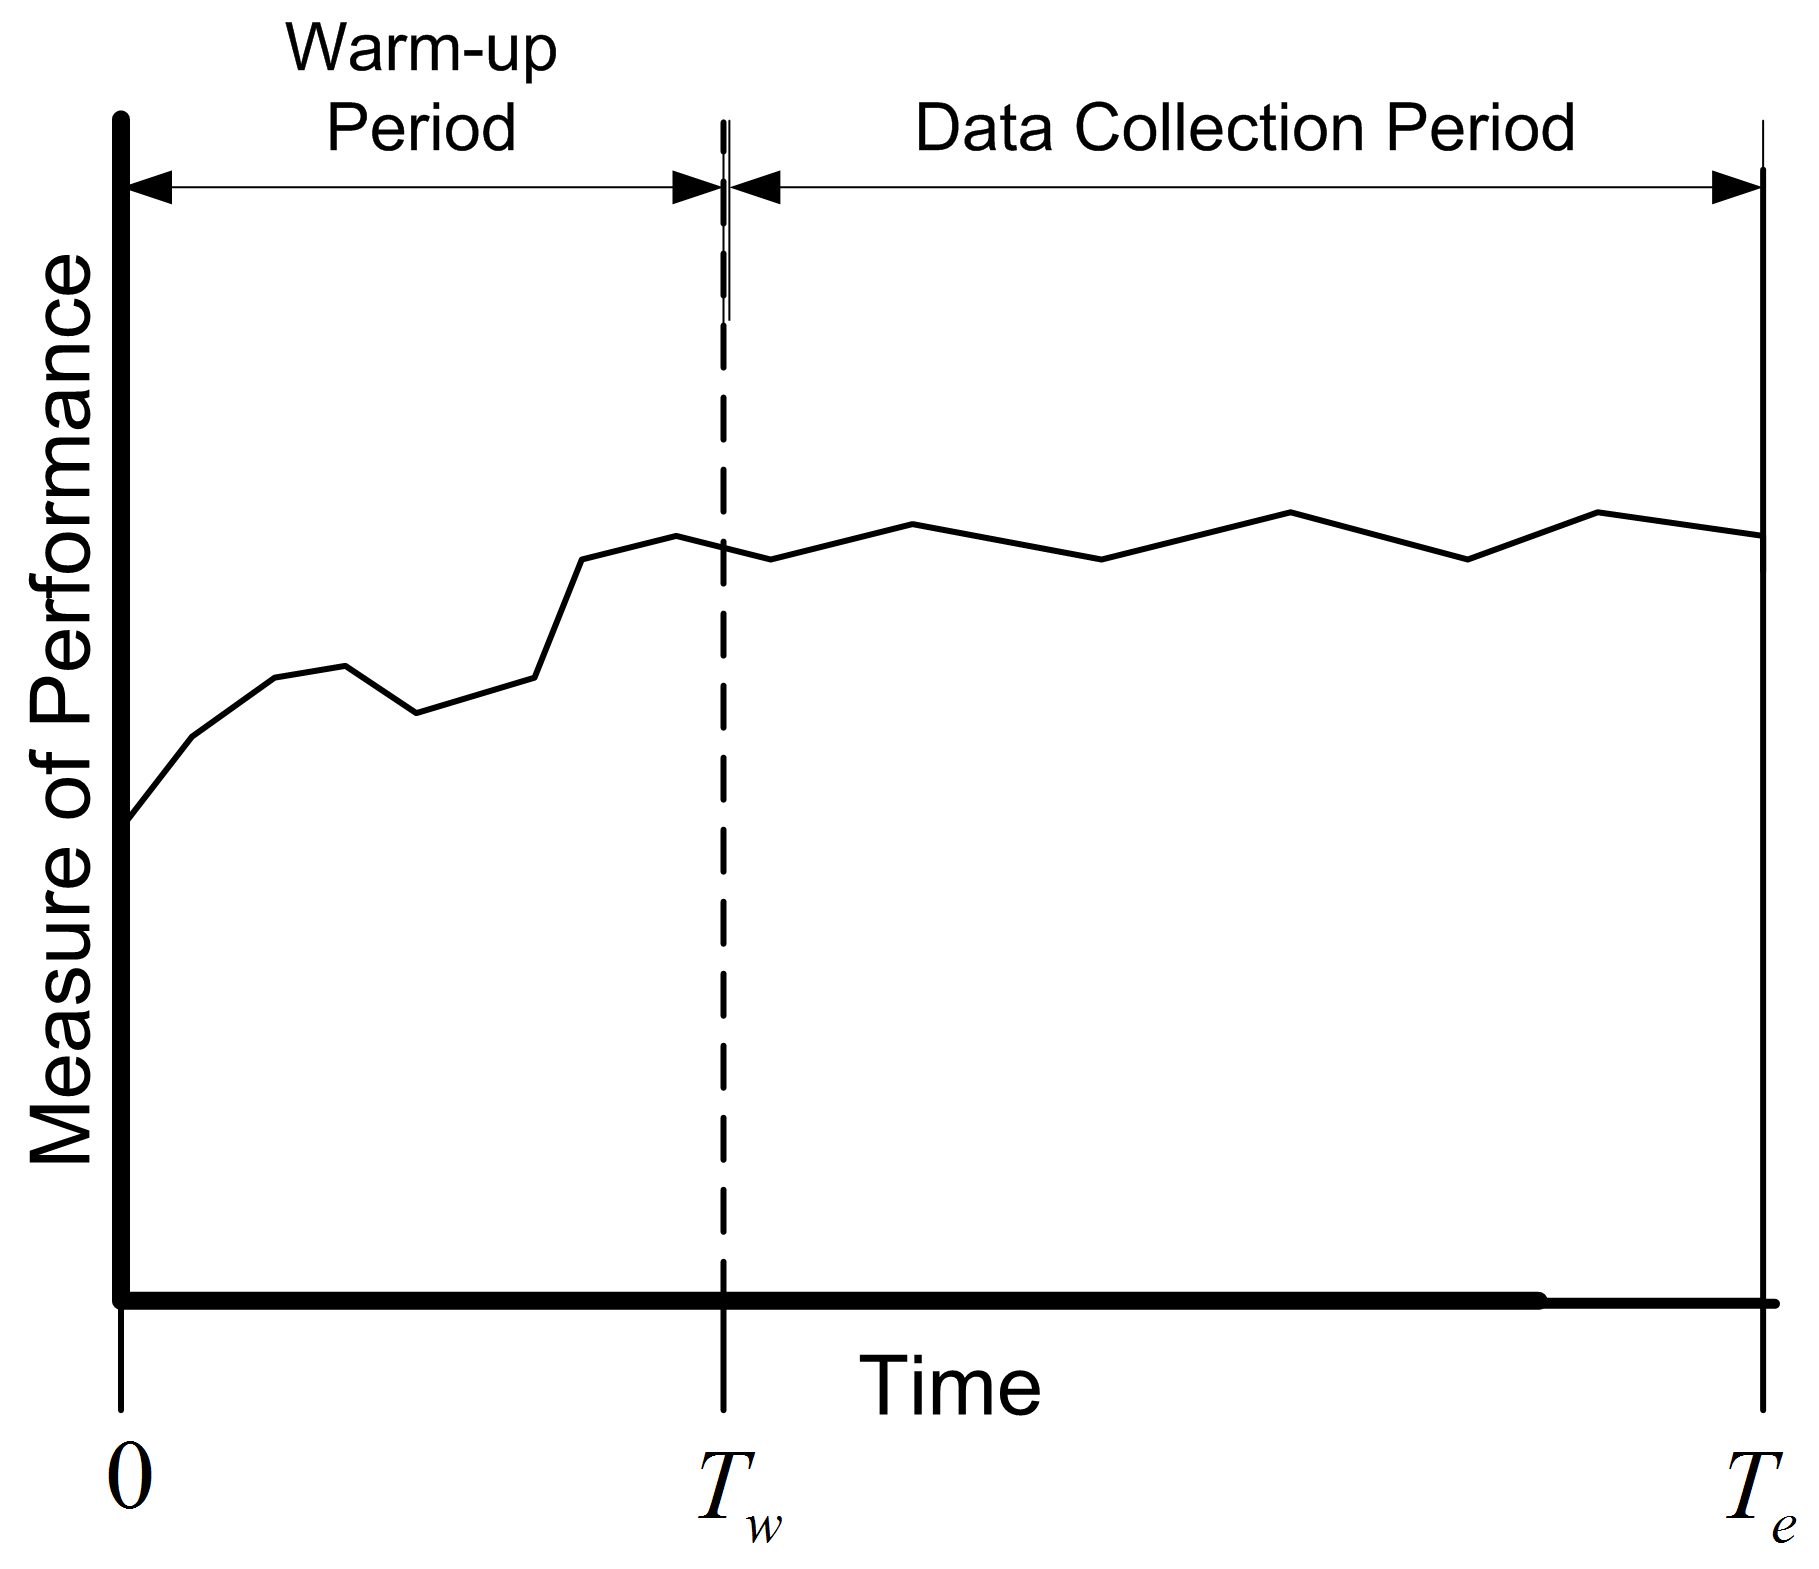
\includegraphics[scale=0.90]{figWarmUpPeriod.png}
\caption{Example of a simulation with warmup period detection. Image from \cite{Manuel}.}
\label{figWarmUpPeriod}
\end{figure}

Fig. \ref{figWarmUpPeriod} show the concept of a warm up period for a simulation replication.
\newpage
\section{Absorbing states}\label{absorbingstate}
%In questo caso dal punto di vista biologico non pu� succedere perch� i nostri geni non degradano.
From a computational standpoint, we could decide to allow an infinite horizon simulation become finite by considering an ending condition that is the absorbing state, that is a state for which all transition rates are zero. This means that there are no transitions that can lead out of that state and, as a consequence, the residency time is infinite.

In our biological context this situation can not happen because if we consider that RNAs molecules are transcripted from a gene and then, from those, proteins and translated and produced, the gene can be in active or inactive form but a gene can not degrade. Hence we will always have at least one molecule and this condition can not happen. In our simulations, however, when comparing the different algorithms, we have considered it as possibile with a rate much lower with respect to the others, for a computational convenience. It is like an additional test that one can do in order to assess that the algorithm works and do not tend to degrade its molecules. 




\part{Studying genetic circuits and noise}

\chapter{Modeling kinetics reactions in a cellular environment}\label{models}
In this chapter, we describe three simple genetic circuits that are common in nature: the simplest process of gene expression and protein synthesis that was already taken into account in the first part (it was exploited to build an hybrid algorithm), the autorepressor case and the toggle-switch model. Hence we need to describe different chemical reactions.

Generally, we can have a chemical reaction like this:
 \begin{equation}
 \ce{\alpha A + \beta B ...
<=> \sigma S + rT}
 \end{equation}
where A and B are the reagents and S and T are the products of the reaction. This reaction is reversible and, as such, according to the \emph{Law of Mass Action}, we can define a \emph{forward reaction rate} and a \emph{backward reaction rate}. The reaction rates are related to a constant, for instance the \emph{forward reaction rate} is related to $k_{+}$, and to the concentration of reagents:
\begin{equation}
 rate = k_{+} A^{\alpha} B^{\beta}
\end{equation}

where $\alpha$ and $\beta$ are called the stechiometric coefficients. Analogously, we can write an equation for the backward reaction rate.

However, the specific forms of these equations rates depend on the order of reaction. In the listed genetic circuits that we will describe, we will consider only first order reaction rates.  

When we have a chemical reaction, we are interested in describing it by using differential equations, hence in a deterministic framework. 

Thus we will turn these biological processes into a deterministic mathematical description, but then the molecular noise in these systems will be taken into account and we will study them by means of stochastic methods.











\section{Constitutive gene expression and Poisson expression statistics}\label{modelconstitutivegeneexpression}
In the simplest possible model of \emph{constitutive} gene expression, a RNA molecule is produced at a constant rate $k_{1}$ and destroyed in a first-order reaction with rate constant $k_{2}$. Fig. \ref{costitutiveexpression} shows a sketch of this simple biological process.

\begin{figure}[!ht]
\centering
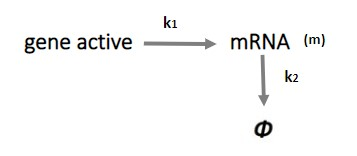
\includegraphics[scale=0.64]{costitutiveexpression.jpg}
\caption{Schematic of a constitutive gene expression model with transcription rate $k_{1}$ and mRNA degradation rate constant $k_{2}$.}
\label{costitutiveexpression}
\end{figure}

As already anticipated in the introductory part, if the total number of a particular transcript \emph{m} is large, the kinetics is conveniently represented as a deterministic differential equation for species concentrations. This plays the role of the mass-balance conservation law, i.e. change = flux in - flux out \cite{geneexpressionnoise}.
\begin{equation}\label{RNAcostitutiveexpressionequation}
 \frac{dm}{dt} = k_{1} - k_{2}m
\end{equation}
This approximation breaks down in cells when the copy numbers of transcripts are small with the need of a probabilistic reformulation in which the conservation law is described by the Chemical Master Equation explained in the previous Chapter \ref{Simulations}. 

In the constitutive expression model, transcript births and deaths occur as uncorrelated events, such that in any short time interval, $dt$, the probability of one transcript production is $k_{1}dt$, and the probability of one transcript degradation is $k_{2}mdt$ \cite{geneexpressionnoise}.

Typically, constitutive genes are the so called ``housekeeping genes'' that are required for the maintenance of basic cellular function \cite{housekeepinggene}, for instance genes coding for ribosomal proteins.

For example, Zenklusen et al. in the experiments \cite{yeastexperiments} found that constitutive gene expression model offers surprisingly good quantitative matches to transcriptional behaviors for the housekeeping genes MDN1, KAP104, and DOA1 in budding yeast. The measured numbers of mRNA transcripts per cell were well described by Poisson distributions for all three genes.

As mentioned in section \ref{theonestepdiscussion} when discussing about one-step processes, from a mathematical point of view, constitutive expression can be seen as a particular case of a one-step process since such molecular reactions are random Poissonian birth-death processes. 

\begin{figure}[!ht]
\centering
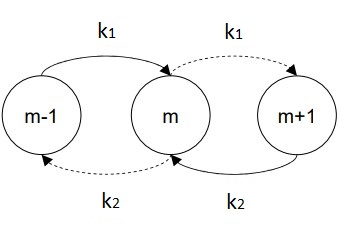
\includegraphics[scale=0.64]{theonestepRNA.jpg}
\caption{For unregulated mRNA synthesis, the system can move into the
state of interest \emph{m} in two ways, indicated by solid arrows. The system can
likewise move out of the state of interest, indicated by dashed arrows.}
\label{theonestepRNA}
\end{figure}

Thus in such case, the distribution of RNA molecules produced has a Poissonian shape.

This is not the case of proteins distribution. The scheme in Fig. \ref{costitutiveexpression} shows only the transcription process in case gene is always active. We can look at this model also considering protein production as shown in Fig. \ref{proteincostitutiveexpression}.

\begin{figure}[!ht]
\centering
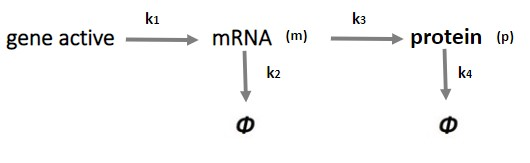
\includegraphics[scale=0.64]{proteincostitutiveexpression.jpg}
\caption{Schematic of a constitutive gene expression model with transcription rate $k_{1}$ and mRNA degradation rate constant $k_{2}$, translation rate $k_{3}$ and protein degradation rate constant $k_{4}$.}
\label{proteincostitutiveexpression}
\end{figure}

Similarly to Eq. \ref{RNAcostitutiveexpressionequation}, we can write the rate of change of protein concentration \emph{p} as:
\begin{equation}\label{proteincostitutiveexpressionequation}
 \frac{dp}{dt} = k_{3}m - k_{4}p 
\end{equation}

The number of proteins produced yields a \emph{scaling law} since they are dependent on both mRNA birth and death as well as translation rates \cite{Article}. Therefore proteins have non-Poisson distributions albeit their scaling is also roughly Poissonian.

\section{Regulated gene expression}\label{regulatedgeneexpressionsection}
Many genes are constitutively expressed at intermediate levels, which represents a permanent cost but provides an immediate benefit when the protein is needed. On the other hand, \emph{regulated} genes are only expressed under certain necessary conditions in order to save cellular energy. In other words, they are switched on only when needed and they be termed also as ``inducible''. Gene regulation is key to the ability of an organism to respond to environmental changes \cite{generegulationNIH}. Fig. \ref{regulatedgeneexpression} shows a sketch of gene regulated protein synthesis model.

\begin{figure}[!ht]
\centering
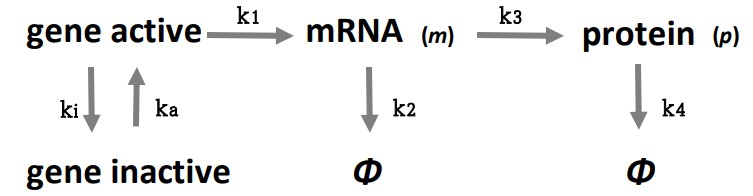
\includegraphics[scale=0.40]{simplest_protein_synthesis_model.jpg}
\caption{Schematic of a regulated gene expression model with gene activation rate $k_{a}$ and gene inactivation rate $k_{i}$, transcription rate $k_{1}$ and mRNA degradation rate constant $k_{2}$, translation rate $k_{3}$ and protein degradation rate constant $k_{4}$.}
\label{regulatedgeneexpression}
\end{figure}

Although the constitutive gene expression model captures the fluctuations of several housekeeping genes, it does not perform as well when gene expression is regulated. Deviations from Poisson behavior indicate regulation. In particular, a two-state model of gene expression can fit this data much better.

This model considers two promoter states: an OFF state, in which no transcription occurs and an ON state, which has transcription rate $k_{1}$. 

The constants $k_{a}$ and $k_{i}$ define the transition rates between the two states, and $k_{2}$ is a first-order rate constant for transcript degradation.

The OFF state is usually associated with a closed chromatin state in which the binding sites for transcription factors are inaccessible, whereas the ON state is associated with the open active chromatin state \cite{geneexpressionnoise}.

And so, a simple way to include transcription factor control in the kinetic equations above is to modify $k_{1}$ using the promoter activity function $g( \cdot )$. Hence, the deterministic equation Eq.\ref{RNAcostitutiveexpressionequation} written for RNA in case of unregulated gene becomes:
\begin{equation}\label{regulatedgeneequation}
 \frac{dm}{dt} = k_{1} \cdot g(\cdot) - k_{2}m
\end{equation}
while the Eq.\ref{proteincostitutiveexpressionequation} for protein keeps unchanged.

$g( \cdot )$ can have different behaviors: in the case shown in Fig. \ref{regulatedgeneexpression}, it makes the gene alternating between active and inactive state. The other two cases that we will study are the autorepressor case and the toggle-switch that now we are going to describe.


%ABBIAMO VISTO GLI EFFETTI DELLA REGOLAZIONE SULLA DISTRIBUZIONE NEL CAPITOLO PRECEDENTE ED ANCHE GLI ANDAMENTI NEL TEMPO.



%Metti tutti i modelli di sintesi proteica:
%unregulated gene
%regulated gene
%autorepressor
%toggleswitch
%informati in quali contesti avvengono.

\section{The Autorepressor model}

As shown schematically in fig. \ref{autorepressor}, in this case gene product represses its own transcription. 


\begin{figure}[!ht]
\centering
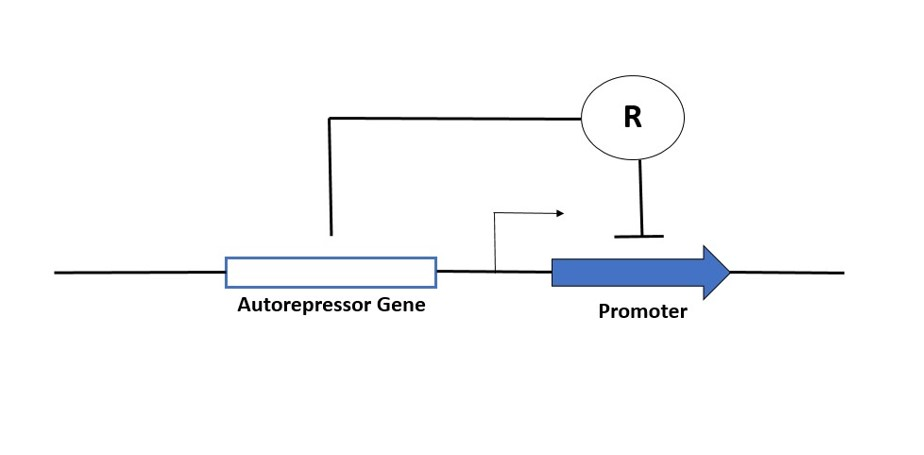
\includegraphics[scale=0.50]{autorepressor.jpg}
\caption{A schematic of an auto-repressing circuit where a blunt line indicates a repressing action while a connector ending with an arrow indicates an activating action}
\label{autorepressor}
\end{figure}

Proteins produced by the gene decreases the rate of activation of the gene. Eq.\ref{regulatedgeneequation} and Eq.\ref{proteincostitutiveexpressionequation} written for the first simple protein synthesis model are then modified in the following way:
\begin{equation}
 \frac{dm}{dt} = k_{1} \cdot g_{R}(r) - \beta_{m}m
\end{equation}
as regards the rate of change of RNA molecules. Analogously, for proteins we can write the same equation as Eq. \ref{proteincostitutiveexpressionequation} written for constitutive expression and for the regulated gene case but, for the sake of clarity, we denote \emph{p} as \emph{r} in order to highlight that protein product is behaving as autorepressor. Hence:
\begin{equation}
 \frac{dr}{dt} = k_{3}m - k_{4}r
\end{equation}

Fig.\ref{autorepressortimeplot} shows the typical pattern of the number of transcript and translated molecoles produced in a genetic autorepressor circuit.

\begin{figure}[!ht]
\hspace*{-2.5cm} 
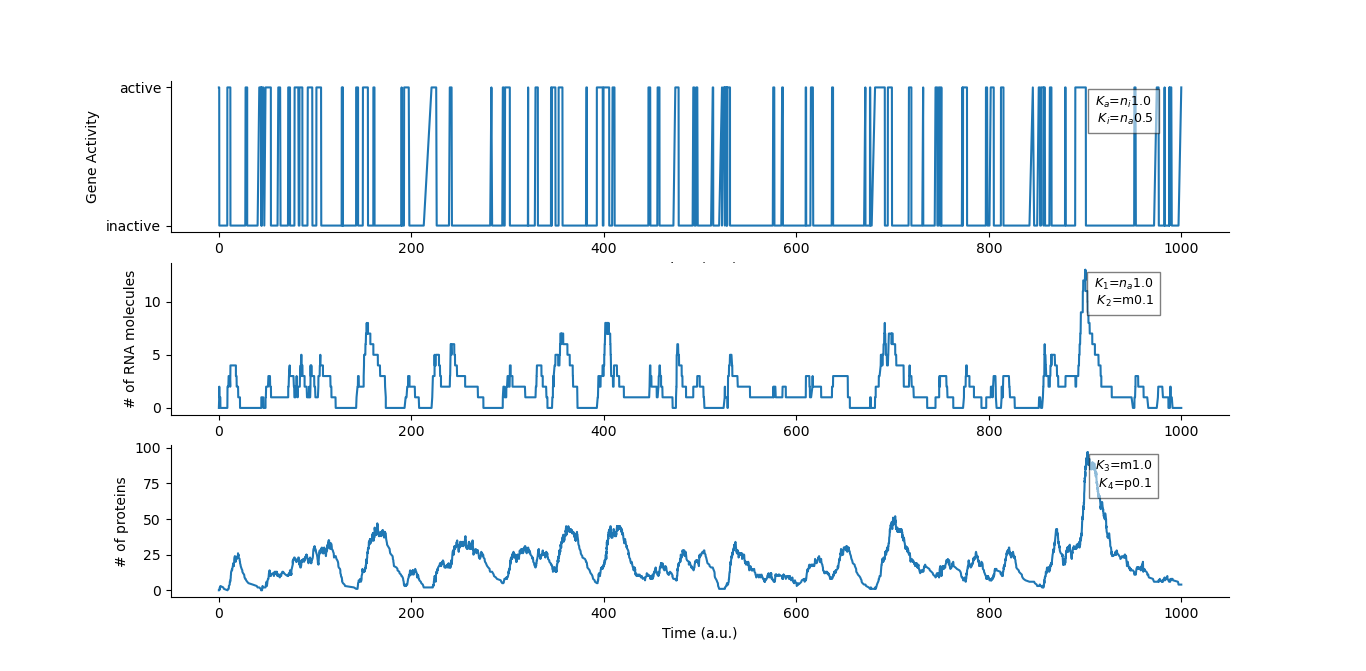
\includegraphics[scale=0.59]{autorepressortimeplotaugeneactivity.png}
\caption{SSA time course simulation of an autorepressor model. The first plot shows the gene activity, the second one the number of RNA molecoles produced and the third one shows the number of proteins produced. Transition rates values are reported in image boxes.}
\label{autorepressortimeplot}
\end{figure}
\newpage
The typical ``sawtooth'' pattern that is repeated over time is revealed by the SSA simulation in RNA molecules trend. As regards proteins time trend, the scaling law mentioned in section \ref{regulatedgeneexpressionsection} causes more ``smooth'' edges. 

One interesting example of autorepressor model in humans is the case of Regulatory Factor $X_{1}$ gene (RFX1).

This gene encodes a member of the regulatory factor X (RFX) family of transcription factors, which are characterized by a winged-helix DNA-binding domain. The encoded transcription factor contains an N-terminal activation domain and a C-terminal repression domain, and may activate or repress target gene expression depending on cellular context. This transcription factor has been shown to regulate a wide variety of genes involved in immunity and cancer, including the MHC class II genes and genes that may be involved in cancer progression. This gene exhibits altered expression in glioblastoma and the autoimmune disease systemic lupus erythematosis (SLE) \cite{RFX1Gene}.

Regulatory factor X1 (RFX1) is an evolutionary conserved transcriptional factor that influences a wide range of cellular processes such as cell cycle, cell proliferation, differentiation, and apoptosis, by regulating a number of target genes that are involved in such processes. On a closer look, these target genes also play a key role in tumorigenesis and associated events. Research work compile significant evidence for the tumor-suppressive activities of RFX1 while also analyzing its oncogenic potential in some cancers \cite{RFX1ArsenalAgainstCancer}.

One of the most understood ways of regulating RFX1's gene expression is by its autorepression. RFX1 auto-represses itself with the assistance of yet unidentified co-repressor, in response to DNA replication arrest, to bring about a controlled expression of RFX1 \cite{RFX1ArsenalAgainstCancer}. Such gene is functionally conserved for instance in yeast where we find a yeast RFX1 homologue, that is Ctr1. There are evidences for a common mechanism for Crt1 and Rfx1 expression and for the conservation of their mode of action in response to a DNA replication block \cite{RFX1genehumansyeast}.




\section{The Toggle-Switch model}
The genetic toggle-switch is a system of two mutually repressing genes. A simplified sketch of this model is shown in Fig.\ref{toggleswitch}.

\begin{figure}[!ht]
\centering
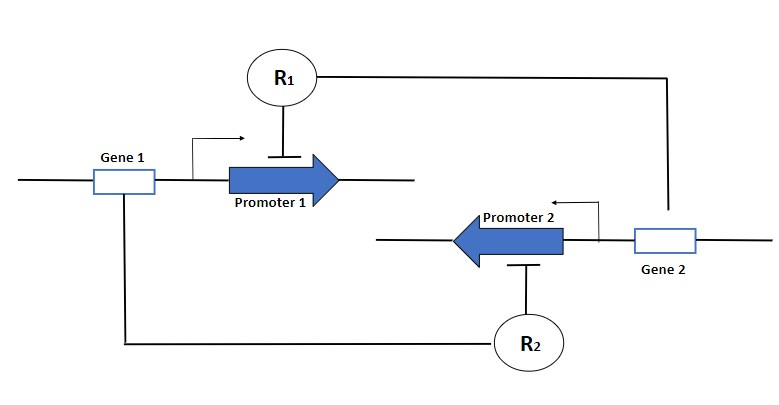
\includegraphics[scale=0.75]{toggleswitch.jpg}
\caption{A schematic of the toggle switch where a blunt line indicates a repressing action while a connector ending with an arrow indicates an activating action.}
\label{toggleswitch}
\end{figure}

The repression of gene 2 is mediated by an inducer (related to gene 1) that regulate gene expression. Similarly this happens for gene 1 repression.

We would expect the system to exhibit \emph{two} mutually exclusive behaviors: either $r_{1}$ is high, keeping expression of $r_{2}$ low, or conversely, $r_{2}$ is high, keeping expression of $r_{1}$ low \cite{SanDiegoUniversity}. 

For simplicity, we assume that the switch is composed of symmetric elements so that the rate constants are identical for each half of the network. Then, as seen in the other cases, the mathematical model takes the form:
\begin{align}
 \frac{dm_{1}}{dt}=k_{1}\cdot g_{R}(r_{2}) - k_{2}m && \frac{dm_{2}}{dt} = k_{1} \cdot g_{R}(r_{1}) - k_{2}m
\end{align}
\begin{align}
 \frac{dr_{1}}{dt}=k_{3}m_{1} - k_{4}r_{1} && \frac{dr_{2}}{dt} = k_{3}m_{2} - k_{4}r_{2}
\end{align}

Fig.\ref{toggleswitchtimeplot} shows the typical trend of gene expression in a toggle switch system.

\begin{figure}[!ht]
\hspace*{-2.5cm} 
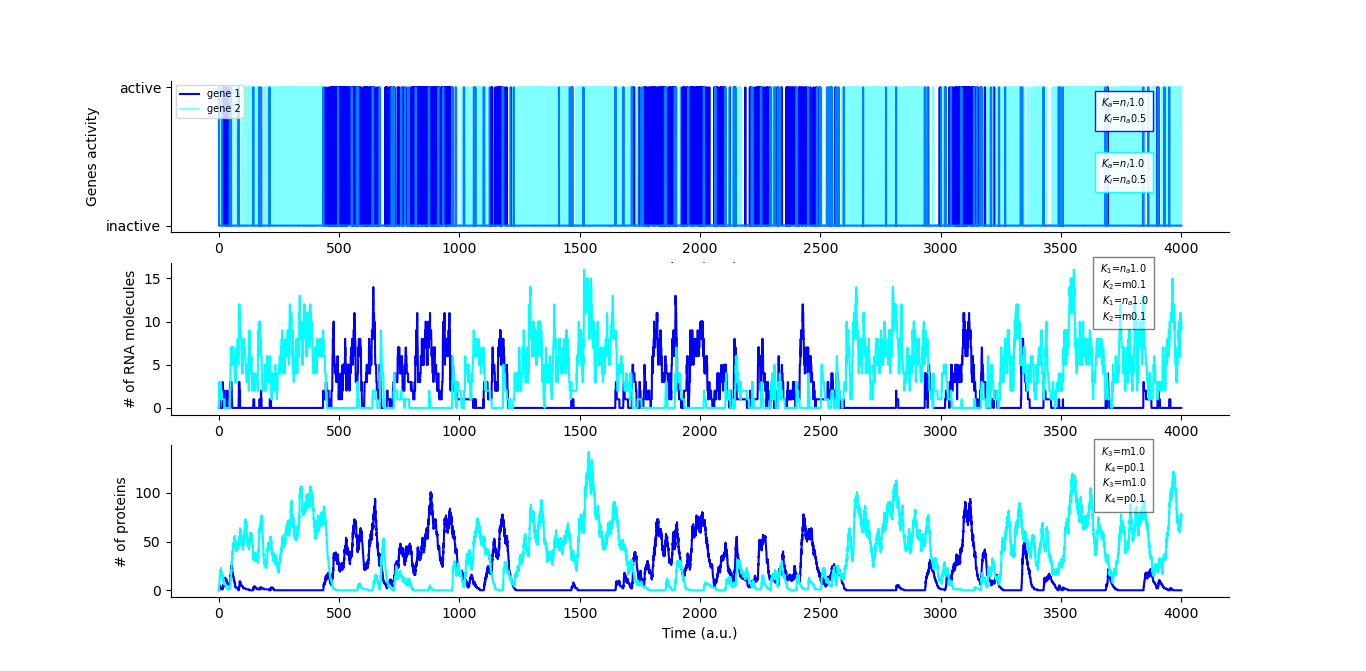
\includegraphics[scale=0.59]{toggleswitchtimeplotaugeneactivity.png}
\caption{SSA time course simulation of a toggle switch model. The first plot shows the gene activity, the second one the number of RNA molecoles produced and the third one shows the number of proteins produced. Transition rates values are reported in image boxes.}
\label{toggleswitchtimeplot}
\end{figure}
\newpage
We can clearly see the alternation between the expression of the two genes.

One example of a genetic toggle switch is the so called MicroRNAs Toggle Switch analysed in the work \emph{
Stochastic analysis of a miRNA-protein toggle switch} \cite{microRNAs} by Giampieri et al.  

MiRNAs are small, non-coding RNAs
that modulate the expression of target mRNAs. MiRNAs are often part of toggle switches, with important examples
are gene pairs built with oncogenes and tumour suppressor genes. The miR-17-92
cluster forms a bistable switch with Myc and the E2F proteins \cite{microRNAs}.



%Ci sarebbe anche il caso di due geni indipendenti

%Dunque mentre nelle prime due configurazioni descritte abbiamo che troviamo questi sistemi tipicamente in determinate situazioni, nel caso dell'autorepressore e toggle-switch non ci sono proprio situazioni tipiche per� nelle situazioni trovate da me sono tipicamente in situazioni in cui sono coinvolti gli oncogenes.

%Useremo come tempo limite 4000 per tutte le analisi perch� come abbiamo visto nel Toggle Switch � il minimo tempo per poter osservare l'alternanza tra le espressioni e per avere una distribuzione Poissoniana nel caso di primo modello di sintesi proteica.

\chapter{Pattern recognition methods for stochastics processes}\label{ChapterPatternRecognition}
We as humans are ``amazing pattern recognizer'' and in fact there are many studies that try to find the link between pattern recognition and human intelligence in order to build artificially intelligent machines \cite{PR}. This is not the theme of this thesis but it is only to say that despite in the time domain signals of Autorepressor model and Toggle Switch model our powerful brain can recognize some patterns, in this context of stochasticity and, perhaps, non-periodic signal, in order to verify that they are really present, and maybe achieve some useful quantitive measurements, we need other tools to investigate such signals than the autocorrelation function that we discussed in section \ref{ACFSubsection}. Let us discuss the ones that we have thought to use in this work of thesis.
%I nostri occhi sono degli ottimi pattern recognizer infatti nell'autorepressore possiamo percepire che c'è qualcosa che si ripete. Abbiamo però bisogno di altri mezzi perchè il segnale nel tempo può nascondere molte features interessanti under the hood. Queste non sempre possono essere svelate dall'autocorrelazione, che come detto nel paragrafo precedente ha come proprietà di cogliere segnali che si ripetono periodicamente nel tempo. Per altri casi possiamo pensare di utilizzare: Transformata di Fourier + quelli elencati dal professore.
\section{Fast Fourier Transform (FFT)}
Our time domain signal, that we can name as $f(t)$, i.e. a function of time, can hide interesting features under the hood and some of these can be extracted through the Fourier Transform. By considering the continous function $f(t)$, the Fourier transform is based on the following formula:
\begin{equation}\label{FourierTransformFormula}
 F(\omega) = \int_{-\infty}^{\infty} f(t)e^{-i\omega t}dt
\end{equation}
the Fourier transform means considering one function of time $f(t)$ and apply a transform, through an integral function, that is the complex exponential $e^{-i\omega t}$ that extracts periodicity from the signal. It is the so called ``inner product'' that is a generalization of the scalar product in which you project one vector onto an other and you see how much of this vector is along an other one. In this case, you can calculate how much of this function $f(t)$ ``is along this function $e^{-i\omega t}$'', so how much of this function $f(t)$ contains the type of periodicity $e^{-i\omega t}$. You can do this for different functions that depend on $\omega$ and you will get a function which depends on $\omega$ that tells you how much is the weight associated to each frequency, hence the frequency domain will tell which is the relative contribution of each frequency into comprising function. We can take \emph{any} function and decompose it into sum of pure waves with different frequencies. The concept was originated by Carl Friedrich Gauss and by Jean-Baptiste Joseph Fourier in the early 19th century. 

Eq. \ref{FourierTransformFormula} considers a continous function. Most of the signals you come across in nature are continuous (electrical signals in your body, human speech, any other sound you hear, the amount of light measured during the day, barometric pressure, etc etc), however, whenever you want to digitize one of these analog signals in order to analyze and visualize it on a computer, it becomes discrete. Indeed our time series of molecules are discretized time series and so they are vectors of values. When both the function and its Fourier transform are replaced with discretized counterparts, it is called the discrete Fourier transform (DFT). The DFT transforms the original $N$-dim data, i.e. it projects onto the new $N$-dim space. Indeed, the FFT $y[k]$ of length $N$ of the length-$N$ sequence $x[n]$ is defined as:
\begin{equation}
 y[k] = \sum_{n=0}^{N-1} e^{-2\pi i\frac{k_{n}}{N}}x[n] 
\end{equation}
and the inverse Fourier transform is then defined as follows:
\begin{equation}
 x[n] = \sum_{n=0}^{N-1} e^{2\pi i\frac{k_{n}}{N}}y[k] 
\end{equation}
In this case, we really are multiplying a signal with a series of sine-waves with different frequencies  and so we are able to determine which frequencies are present in a signal. If the dot-product between our signal and a sine wave of a certain frequency results in a large amplitude this means that there is a lot of overlap between the two signals, and our signal contains this specific frequency. This is of course because the dot product is a measure of how much two vectors / signals overlap.

The DFT has become a mainstay of numerical computing in part because of a very fast algorithm for computing it, called the Fast Fourier Transform (FFT). It makes use of the symmetry of the sine and cosine functions and other math shortcuts to get the same result much more quickly.

Thus, the Fourier analysis tells us how much of data is organized as function of \emph{frequency} and no more as function of \emph{time} so it is used to transform a signal from a time domain to a frequency domain.

Fig. \ref{exampletimedomainsignal} is an example of a signal that contains four different frequencies at four different times.

\begin{figure}[!ht]
\centering
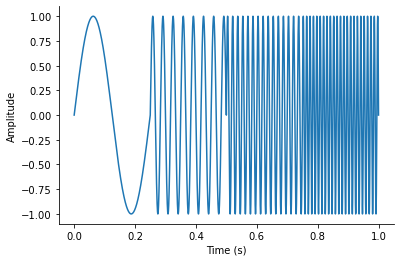
\includegraphics[scale=0.80]{examplesignalchangesfrequency.png}
\caption{Example of time domain oscillating signal which contains four frequencies at four different times.}
\label{exampletimedomainsignal}
\end{figure}

Fig. \ref{exampleFFTtimedomainsignal} is the corresponding frequency spectrum.

\begin{figure}[!ht]
\centering
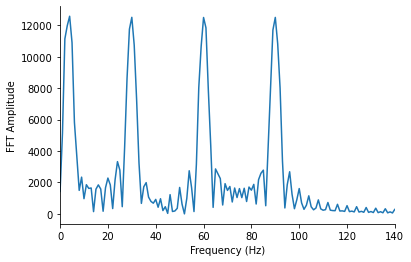
\includegraphics[scale=0.80]{exampleFFTsignalchangesfrequency.png}
\caption{Example of FFT applied to the signal in figure \ref{exampletimedomainsignal}.}
\label{exampleFFTtimedomainsignal}
\end{figure}

The four frequencies, already clearly detectable by eye in the time domain, are all present in the frequency domain. The peaks in the frequency spectrum indicate the most occurring frequencies in the signal. The larger and sharper a peak is, the more prevalent a frequency is in a signal. 


%Non so più se è giusto...
However, as in the case of the autocorrelation function, if the signal is not periodic, the Fourier spectrum would not be really informative. The sine function is the same everywhere, no matter where you look. It stretches to infinity in a regular periodic fashion which meakes it inconvient for time series analysis. Indeed we can say that the autocorrelation function and the Fourier transform are two ways to obtain the same information from the signal: the extraction of periodicity from the signal. Computing the autocorrelation function we obtain a graph with the autocorrelation values as function of time; with the Fourier transform we obtain the FFT amplitude as function of frequencies. Converting the values of the autocorrelation peaks from the time-domain to the frequency domain should result in the same peaks as the ones calculated by the FFT. The frequency of a signal thus can be found with the auto-correlation as well as with the FFT and this was already mentioned in a more ``formal'' way in section \ref{ACFSubsection} as a result of the \emph{Wiener-Khinchin theorem}.

%AGGIUSTA!!!!!!!!!!

Furthermore, from these figures and from the FFT theory explained before, we can understand that this approach has an important drawback: the Fourier Transform has a high resolution in the frequency-domain but zero resolution in the time-domain. This means that it can tell us exactly which frequencies are present in a signal, but not at which location in time these frequencies have occurred. It is fundamentally impossible to have both: time and frequency resolution simultaneously. There is always a trade off of information between the two. This is a manifestation of the \emph{Heisenberg uncertainty principle}. Time and frequency are two extremes of these uncertainty: you can either know exactly what a value of a function is at every time point but at the cost of being completely ignorant about what frequencies are fold in. On the other hand, in the frequency domain we know exactly what frequencies are present in that signal but we have no idea about the temporal dynamics of them. A compromise that would sacrify a little bit of frequency resolution and a little bit of time resolution to know something about both is the Wavelet transform.




\section{Continous Wavelet Transform (CWT)}
The Fourier transform uses sine and cosine waves with different frequencies but with the same shape along all the time domain and they repeat periodically back and forth in time. The Wavelet transform instead uses a series of functions called wavelets which have a beginning and an end. The french word wavelet means ``a small wave'', and this is exactly what a wavelet is. Hence while the sine and cosine waves are infinitely long and stretches to infinity in a regular periodic fashion, the Wavelets are \emph{localized} in time and with a different shape. This allows the wavelet transform to obtain time information in addition to frequency information.

Indeed, since they are localized in time, this transform implies that we can multiply our signal with the wavelet at different locations in time. The wavelet is thus translated from the beginning to the end of the signal (i.e. the time series). This operation is named as \emph{convolution}. In this way, you are localizing along the time series the value of this finite domain function. The process is illustrade in the fig. \ref{exampleofconvolution}:

\begin{figure}[!ht]
\centering
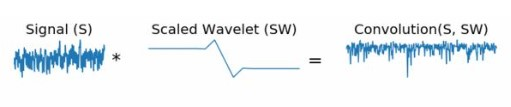
\includegraphics[scale=0.80]{exampleofconvolution.jpg}
\caption{Sketch of Wavelet transform applied to the signal through convolution. Image from \cite{WaveletsTutorial}.}
\label{exampleofconvolution}
\end{figure}
The wavelet can then also be scaled by dilations and contractions. Furthermore, there are different families of wavelets each one characterized by a specific shape. For instance, we can consider the so called Morlet wavelets that are frequently used for time-frequency analysis of non-stationary time series data, such as neuroelectrical signals recorded from the brain \cite{Neuroscience}. Fig. \ref{Morlet} shows three different pictures that show the same wavelet function represented using different scales.

\begin{figure}[!ht]
\centering
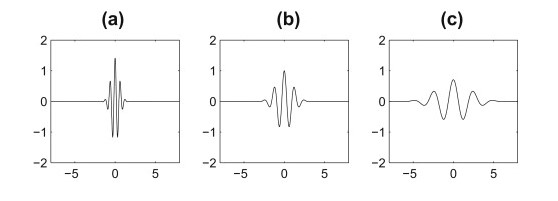
\includegraphics[scale=0.80]{Morlet.jpg}
\caption{Morlet wavelet at three different scales: (a) contracted wavelet, (b) mother wavelet, (c) dilated wavelet. Image from \cite{ScienceDirectMorlet}.}
\label{Morlet}
\end{figure}
Using a wavelet function like this you will identify in the time series positive and negative parts.

Mathematically, we can summerize all this with the following formula that represents the Continous Wavelet Transform (CWT):
\begin{equation}\label{CWT}
 CWT(a,b) = \frac{1}{\sqrt{a}}\int_{-\infty}^{+\infty} Y(t)\psi\left(\frac{t-b}{a}\right)dt 
\end{equation}
In this equation, the parameter \emph{a} is the scaling factor that stretches or compresses the function. The parameter \emph{b} is the translation factor that shifts the mother wavelet along the axis. The parameter $Y(t)$ is an integrable signal whose sum is to be multiplied by the translated mother
wavelet. And finally, the mother wavelet is denoted by $\psi(t)$, which is a function of the scaling and translation factors just as the result of the continuous wavelet transform is.
%+SE HAI TEMPO METTI LA DIFFERENZA TRA CWT E DWT.


Generally speaking, to be considered a proper wavelet, a function $\psi(t)$ has to satisfy two main constraints:
\begin{enumerate}
 \item \begin{equation}
        \int_{-\infty}^{+\infty}  \psi(t)dt = 0
       \end{equation}
 \item \begin{equation}
        \int_{-\infty}^{+\infty}  |\psi(t)|^{2}dt <  \infty
       \end{equation}
\end{enumerate}
The first one is known as the ``admissibility condition'' and it tells that the wavelet function should have zero mean. This means that if you take the integral, i.e. the area under the curve, and we sum the positive and negative parts, we should get zero. We can notice that also a sine wave passes the admissibility condition. Secondly, the wavelet function has to have finite energy: if you square the function and compute the area under the curve everywhere from minus infinity to plus infinity it should be a finite number and this exactly what makes the function localized in time. It means that the wavelet covers a finite area. In fact think about the energy of the sine wave: it is infinite.

As said before, one very known wavelet is the Morlet wavelet that is defined taking the cosine wave of a certain frequency and damping it by multiplying on a Gaussian bell curve:
\begin{equation}\label{MorletEquationFormula}
 \psi(t) = k_{0}\cos(\omega t)e^{-\frac{t^{2}}{2}}
\end{equation}
this is the \emph{real} component of a Morlet wavelet and has the shape depicted in fig. \ref{Morlet}. Wavelet itsself is a complex function and we will discuss about this in a few.


Hence, in this case, when doing the Wavelet transform we have to choose the \emph{scale} and the \emph{mother wavelet} to use that will be \emph{translated} and multiplied to the signal. By varying scale and translation parameters we can ``scan'' our signal with analysing wavelets of different scales to see what frequencies are most prominent around that time point.

The Wavelet transform gives, in any case, information about local periodicities and so how frequencies in a time series data are localized in time. However, the best choice of the parameters just mentioned is able to give more informative results.

We can consider an example of the application of the CWT to the signal rappresented in fig. \ref{exampletimedomainsignal} that changes its frequency at four different time steps. A good tool for the CWT representation of our signal is the \emph{scaleogram}. It is a 2D representation of a 1D signal in time domain. The scaleogram, as the name suggests, reports the time on the horizontal axis and the period, i.e. the length of the Wavelet or also called the scale, one the vertical axis. For our convention, the color-level coded scale represents the wavelet coefficients: dark red is associated to high values of wavelet coefficents, while white colored regions represent low values of wavelet coefficients. To clarify, by ``wavelet coefficients'' we mean the result of the convolution between the time series and the chosen wavelet, just as the FFT amplitude values in the Fourier transform. 

On the vertical axis of the scaleogram we put the scale, that the wavelet length: higher the length of the wavalet is, lower the frequency is; on the contrary, lower the length of the wavelet is, higher the frequency is.

\begin{figure}[!ht]
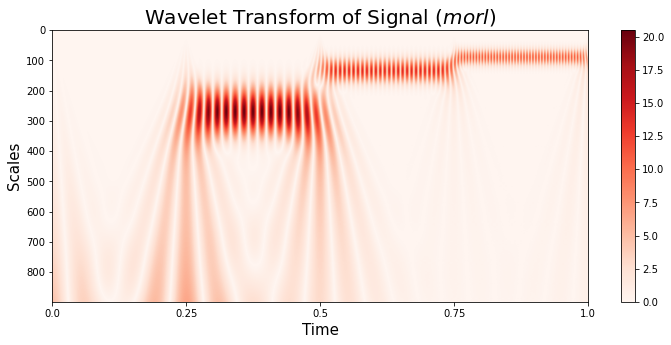
\includegraphics[scale=0.59]{MorletTransformSignalExample.PNG}
\caption{Example of Continous Wavelet Transform, using the real part of Morlet wavelet, applied to the signal in figure \ref{exampletimedomainsignal}.}
\label{MorletTransfromSignalExample}
\end{figure}

Hence, how do we interpret the scaleogram ? Roughly speaking, the convolution measure the similarity between the wavelet function and the data. If the similarity is high, we will have high values of wavelet coefficients (i.e. red colors); if it is low, it will correspond to low wavelet coefficients (i.e. like white colors). But since wavelets vary from one scale to an other, at certain scales it may or may not have the highest similarity. If at low scales (low values on the vertical axis of the scaleogram) there are high values of the coefficients, then the data have high frequencies; on the other hand, if at high scales there are high values of coefficients, then your data have low frequencies. Thus we can locate this low and high frequency portions by analysing these variations in the values of the coefficients. When there is no match with the signal, the dot product, i.e. the result of integral in Eq. \ref{CWT} is zero; but when the signal approaches the wavelet intrinsic frequency, the function begins like to ``resonate'' and you get a significant overall contribution when they are in phase, and a significant negative contribution when they are out of phase. When there is match of frequency there is an alternation between positive and negative values. We can realize that Eq. \ref{CWT} is exactly as the dot product between vectors, indeed when vectors have the same direction, the dot product has high value, contrary to when the angle between them is $90^{\circ}$ in which case it is zero or when they have opposite directions in which case it has negative value.

Fig. \ref{MorletTransfromSignalExample} shows the Morlet CWT applied to signal in fig. \ref{exampletimedomainsignal} that changes frequency at four time points. Such scaleogram generally shows bands made of an alternation between red and white stripes. In particular there are four bands of this type that are located at lower and lower scale corresponding to the time domain signal that increases its frequency.

However we need to notice that the product in Eq. \ref{CWT} is zero also when the wavelet is exactly in the middle between peaks and troughs of the oscillating signal. It does not mean that there is zero frequency component , but it could be quite the contrary. 
%of the resulting oscillation of convolution values. 
%So since we want to measure the contribution of frequency as function of time is to take the envelope of the Morlet wavelet

This is when complex wavelets come into play. If we consider again the Morlet wavelet defined in Eq.\ref{MorletEquationFormula}, we obtain the complex Morlet wavelet multiplying it by $e^{i\omega_{0}t}$ and so we obtain:
\begin{equation}
 \psi(t) = k_{0}\cos(\omega t) e^{i\omega_{0}t} e^{-\frac{t^{2}}{2}}
\end{equation}
In this way the Morlet wavelet is essentially a complex exponent which spins around the circle in the complex plane with a certain constant frequency $\omega_{0}$ and whose amplitude is modulated by the Gaussian bell curve $e^{-\frac{t^{2}}{2}}$. 

The imaginary part of the Morlet wavelet is like the real part but slightly shifted relative to the cosine. The key idea is to calculate the convolution with both real and imaginary parts.  Then our convolution function, for a fixed wavelet scale, will map one real number to the point in the complex plane where the real component is the value of the convolution at that time point with the real part of the wavelet and the imaginary component is the value of convolution with the imaginary part of the wavelet. The power of the frequency, i.e. the intensity of its contribution, at each point in time is given by the distance from the resulting point in the complex plane to the origin which is the \emph{absolute value of the complex number}. In this way we measure the intensity of a particular frequency component as function of time. The resulting function Eq. \ref{CWT} is the complex function, the absolute value of which represents the contribution of a particular frequency around a certain time point. We can again represent it with colors obtaining the scaleogram.

Fig. \ref{ComplexMorletTransfromSignalExample} shows the scaleograms corresponding to CWT applied to signal in Fig. \ref{exampletimedomainsignal} using the complex Morlet wavelet. At first sight, we can understand that this graph is more intuitive than the one obtained through only the real part of Morlet wavelet that was shown in Fig. \ref{MorletTransfromSignalExample}.

\begin{figure}[!ht]
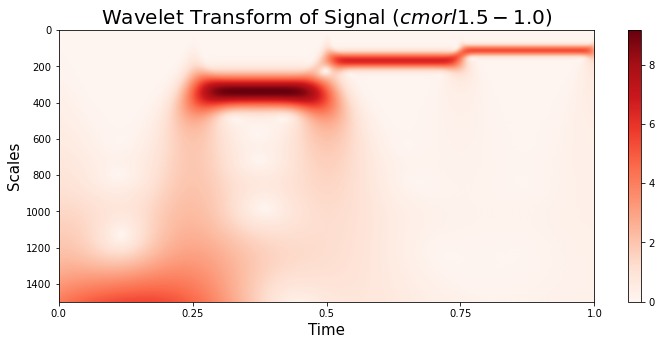
\includegraphics[scale=0.59]{ComplexMorletTransformSignalExample.PNG}
\caption{Example of Continous Wavelet Transform, using Complex Morlet wavelet, applied to the signal in figure \ref{exampletimedomainsignal}.}
\label{ComplexMorletTransfromSignalExample}
\end{figure}

Fig. \ref{ComplexMorletTransfromSignalExample} shows four different bands located at four different time points and at four different scales. This time, the bands are uniformly dark red colored and this agrees with our expectations since the time domain signal changes its frequency four different times by increasing its frequency.

Before concluding this overview about wavelets, we need to emphisize that the results may change according to the choice of scale and the choice of the wavelet used. The first one is obvious: by considering a lower range of scales in a situation like this, we would not have detected the lowest frequency present at the beginning of the signal. However, this is true if we use a Complex Morlet Wavelet. 

Indeed, in a situation like this, if we apply the Complex Gaussian Wavelet transform to the usual signal in Fig.\ref{exampletimedomainsignal}, we are able to detect low frequency signal by using a lower range of scales.

\begin{figure}[!ht]
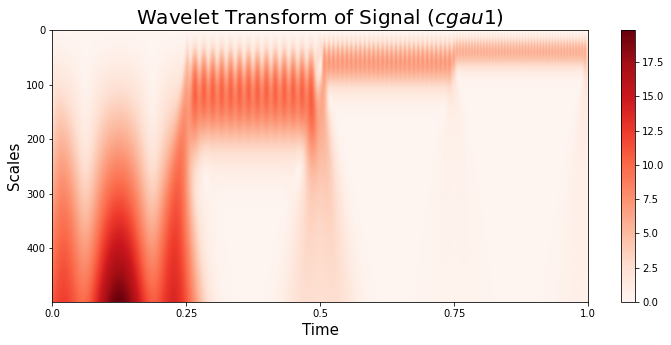
\includegraphics[scale=0.59]{ComplexGaus1TransformSignalExample.PNG}
\caption{Example of Continous Wavelet Transform, using Complex Gaussian wavelet of first order, applied to the signal in figure \ref{exampletimedomainsignal}.}
\label{ComplexGaus1TransformSignalExample}
\end{figure}
\newpage
From these pictures, we can recognize the power of the CWT for dynamically changing signals in recognizing frequencies present in the signal together with their temporal localization. Furthemore, as pointed out previously, we can notice also the importance of the parameters chosen which in this case is the choice of the wavelet. 

%We have shown three scaleograms based on three different wavelets and each one has been capable to give different type or a different ``amount'' of information.  



%Mouse brain signal: Wavelet transform can help us discover its structure. There are three distinct bouts of low frequency rhythm with a gradual decrease in frequency and we can easly quantify the frequency and the duration of each of those patterns. Additionally each of them is associated with several bouts of higher frequency rythm and their frequency follows the bell shape. We can objectively quantify all sorts of parameters such as their frequency values, durations, the rise and decay of the frequency modulation and so on. The possibilities are endless.

%As regards the inherent trade off between time and frequency resolution that you can not know both. Does the wavelet transform violet the uncertainty principle ? If you look closely at the wavelet scalogram of a sine wave you will see that even for a signal consisting of a pure wave the resulting image does not look as infinitely narrow bar as it would be for a Fourier transform instead it looks kind of blurred. That's because we loose resolution in both time and frequency to know something about both. 

%La rappresentazione con i numeri complessi ti permette di ruotare nel piano complesso in modo facile.

%Figure TOT IS WITH GAUSSIAN WITH SCALE TOT. THE OTHER FIGURE TOT IS WITH LOWER SCALE THAT MEANS HIGHER FREQUENCIES.

%PENSO CHE TRASLA E POI FA UNA NUOVA TRASLAZIONE CON UN NUOVO VALORE DI SCALA DATO DALLA LISTA DI SCALE.

\newpage

\section{ACF, FFT and CWT applied to the first protein synthesis model}

Most of the time, the structure of data is hidden behind the noise so we need these precise mathematical operation with which we can look through the noise and quantify the structure present in the signal. Wavelets are something like could do this blurring of vision and zoom in and out of the signal to pull out the patterns like a kind of mathematical microscope.
%Metti discorsi fatti dal 2 Novembre in poi e le novit� sull'autocorrelazione delle differenze.
%La trasformata di Fourier media ed analisi di ogni picco per trovare il rate con cui sono prodotte le molecole e le wavelet transform. Usiamo tale modello perchè è il più semplice quindi come Toy model. 
%Autocorrelazione delle differenze.
%Questo lavoro di caratterizzare la forma di una funzione di autocorrelazione per ogni modello pu� essere utile nel momento in cui ho i dati sperimentali, ne calcolo l'autocorrelazione e se vedo un deep per esempio posso dire che c'� una forma di repressione.
%DEVI METTERE PRIMA LE CURVE DI AUTOCORRELAZIONE DI PIù SIMULAZIONI PER CAPIRE QUALE CRITERIO ADOTTARE PER LA RAPPRESENTAZIONE CON I QUANTILI PIù FORMALE. 

\section{ACF, FFT and CWT applied to Autorepressor signals}
%ACF: se hai un delay di 1000 punti corrisponde a 10 secondi virtuali, se invece dt=1 e lag 1000 punti sono 1000 secondi virtuali messaggio.
As we have discussed in Chapter \ref{models}, the autorepressor is a little genetic circuit with negative feedback. The gene\textquotesingle s proteins product decreases the activation rate of the same gene. We have also observed a typical trend as function of time in Fig.\ref{autorepressortimeplot}.

At first sight, there is a sawtooth pattern that is repeated over time in the number of RNA molecules vs time trend, whereas the proteins trend is characterised by more ``smoothed'' edges.

This first impression finds a sort of confirmation by the autocorrelation plots:

\begin{figure}[!ht]
\centering
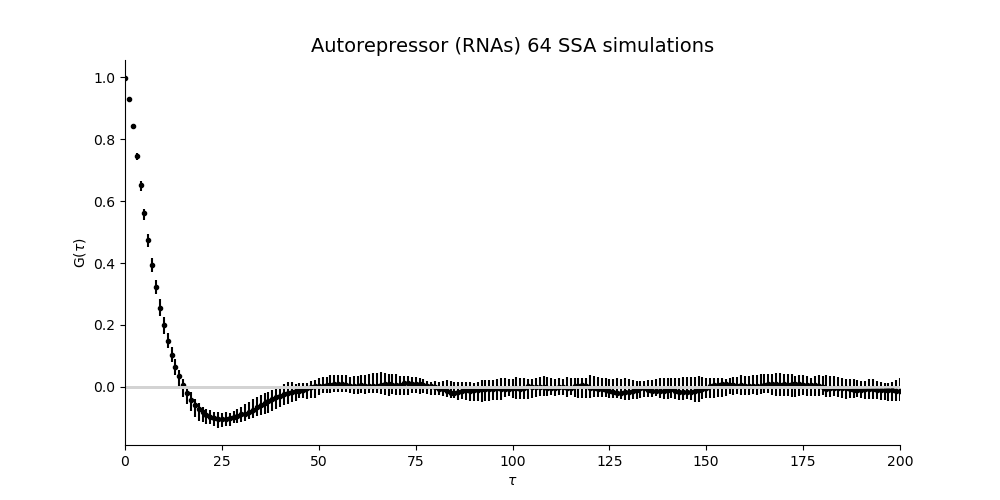
\includegraphics[scale=0.60]{AutorepressorRNAsACFnlags2000dt1nsimulations64.PNG}
\caption{Trend of RNAs autocorrelation plot as function of sampling time as a result of 64 simulations. The number of lags used to calculate the autocorrelation is 2000 with a sampling time dt=1. The error bars  and the points are respectively calculated by considering the 25\% or 75\% quantiles and the median.}
\label{AutorepressorRNAsACFnlags2000dt1nsimulations64}
\end{figure}
\newpage
Fig. \ref{AutorepressorRNAsACFnlags2000dt1nsimulations64} shows an autocorrelation curve that is the result of 64 simulations. It is characterized by a deep at the first virtual time points and then it tends to zero. We can clearly see this from the overlapping between the horizontal line at zero and the autocorrelation points or the relative error bars.

We expected the negative deep because of the repressing behavior. Also in the analogous proteins autocorrelation plot (see Fig. \ref{AutorepressorProteinsACFnlags2000dt1nsimulations64}) we can find a similar trend but in this case we find ``a less profound deep'' that maybe due to the smoothed time course behavior.
\newpage
\begin{figure}[!ht]
\centering
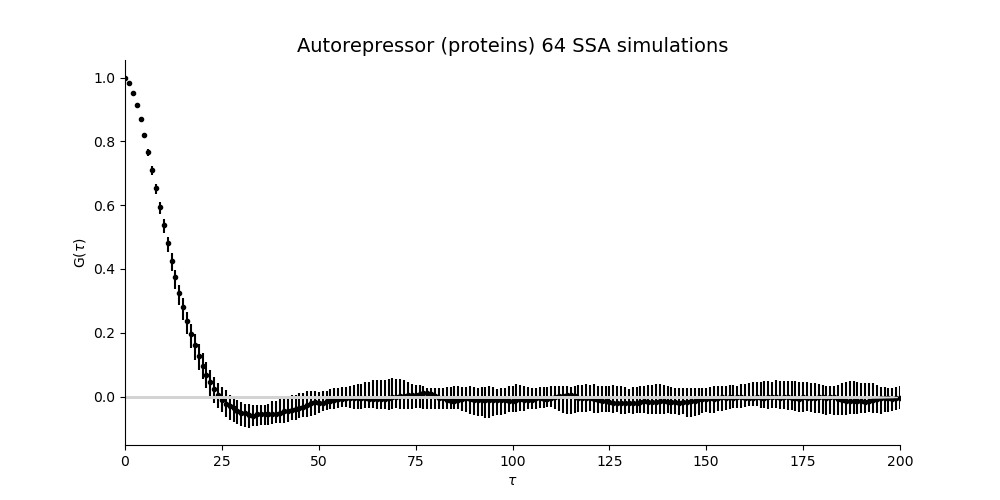
\includegraphics[scale=0.60]{AutorepressorProteinsACFnlags2000dt1nsimulations64.PNG}
\caption{Trend of proteins autocorrelation plot as function of sampling time as a result of 64 simulations. The number of lags used to calculate the autocorrelation is 2000 with a sampling time dt=1. The error bars  and the points are respectively calculated by considering the 25\% or 75\% quantiles and the median.}
\label{AutorepressorProteinsACFnlags2000dt1nsimulations64}
\end{figure}

This shows how the autocorrelation function is really sensitive to the shape of the molecular time course behavior.  

\newpage




\section{ACF, FFT and CWT applied to Toggle-Switch signals}

\part{Deep Neural Networks for parameters estimation}
%Noi usiamo l'autocorrelazione per� possono essere usate altre funzioni dipendenti dai parametri del sistema. Tipo alcuni usano lo scaleogramma. Trova le fonti che interessava molto il professore. 
\chapter{Artificial Neural Networks as data-driven modeling}
The regression problem is how to model one or several dependent variables/responses, \emph{Y}, by means of a set of predictor variables, \emph{X} \cite{datadrivenmodeling}. 

This problem can be faced in the data-driven modeling framework that is often more suitable to describe the real-world systems that are associated with complexities. A data-driven model is based on the analysis of the data about a specific system. The main concept of data-driven model is to \emph{find relationships between the system input and output variables without explicit knowledge of the physical behavior of the system} that is, in few words, the opposite of what we did in the previous sections when modeling genetic circuits. Unlike first principles models, data-driven models make no attempt to model the internal features of the system. Instead, they focus on matching the input-output behavior to observational data. 

The input-output data available from a system can be used to derive different forms of computationally efficient data-driven models for the purpose of prediction, state estimation, monitoring, and other process systems engineering applications. The rapid increase in the availability of data of physical systems has stimulated the development of many data-driven methods for modeling and prediction. 

In this thesis we use Artificial Neural Networks (ANN) as a method of data-driven modeling class. We use as input data the autocorrelation function whose shape depends on the system parameters and the output data are, indeed, the constant rates of reactions. Hence, it is a matter of building a multi-output regression model using a supervised deep neural network. Then this can be exploited for the purpose of state estimation.

First we will describe the basics artificial neural networks concepts and then we will apply them to the data just mentioned that regard the three genetic models we studied. The results are both important for the building of a data-driven model that is applicable to experimental data and also the building of such deep learning model reveals biological important features of the simple genetic circuits we analysed. Even this last feature can be considered when dealing with data coming not from simulations. 

\section{Artificial Neural Networks: the basic principles}

\section{Building a Neural Network regression model}

\section{Particular Artificial Neural Networks: Recurrent Neural Networks (RNN) and Long Short Term Memory (LSTM) Networks}

\chapter{Artificial Neural Network regression model at work}
%The widely used ANN paradigm is a multi-layered feed-forward network (MFFN) with multi-layered perceptron, mostly comprising three sequentially arranged layers of processing units. The MFFN provides a mapping between an input (x) and output (y) through a nonlinear function f as y=f(x). The three layered MFFN has input, hidden, and output layers, and each layer comprises of its own nodes. METTICI PER� CHE NON SAPPIAMO QUAL'� LA FUNZIONE f E LE COSE SCRITTE NEL PROGETTO DI REMONDINI. + USA IN QUALCHE MODO LE LSTM. 
\section{ANN applied to the first protein synthesis model}
\section{ANN applied to the Autorepressor model}
\section{ANN applied to the Toggle-Switch model}
%Confrontare la mae e la r2score generati da modelli uguali con diverse specie chimiche può darci informazioni su tali specie.

\part{NF-\texorpdfstring{$\kappa$}{\265}B, a stochastic active player in human cancer}
\chapter{The NF-\texorpdfstring{$\kappa$}{\265}B family of transcription factors}

%METTI COSA SONO I FATTORI DI TRASCRIZIONE.

%More than years ago, Ranjan Sen and one of the authors did a series of experiments that identified a protein binding to a specific, conserved DNA sequence in nuclei of activated B lymphocytes. They named it for the cell type in which they identified it and the gene it affected: Nuclear Factor binding near the $\kappa$ light chain gene in B cells and so it is called NF-$\kappa$B. The Ig-light (IgL) chains ensure the expression and secretion of functional antibodies and contribute to antigen binding by increasing the variability of the antibodies. It was realized that NF-$\kappa$B would have a wide role in inflammation and other natural and pathological processes.

Nuclear factor kappa-light-chain-enhancer of activated B cells (abbreviated as NF-$\kappa$B) was originally identified as a family of transcription factors that bind the enhancer of the immunoglobulin $\kappa$ light-chain gene, whose function is to ensure the expression and secretion of functional antibodies and contribute to antigen binding by increasing the variability of the antibodies \cite{immunoglobulin}. This was discovered by Ranjan Sen and his collegues in their experiments that identified a protein binding to a specific, conserved DNA sequence in nuclei of activated B lymphocytes. They named it for the cell type in which they identified it and the gene it affected: Nuclear Factor binding near the $\kappa$ light chain gene in B cells \cite{nfkb30years}. Although its function in the regulation of immunoglobulin light-chain gene remains unclear, NF-$\kappa$B plays critical roles in development, survival, and activation of B lymphocytes \cite{Immuno}. So it has been considered key regulator of antibodies production. 

However, NF-$\kappa$B has been found in all cell types implicated in the transcriptional events controlling multiple cellular outputs. It comprises a family of structurally-related eukaryotic transcription factors, which bind to consensus DNA sequences at promoter regions of responsive genes regulating a large number of normal cellular and organismal processes such as immune and inflammatory responses, developmental processes, cellular growth and apoptosis and, for such reason, its name contains information not completely correct since it is neither a fundamental regulator of $\kappa$ light-chain gene nor B-cell specific.

Nowadays, NF-$\kappa$B is actually considered as a pleiotropic mediator of gene expression control. 

%Experimental results led to the identification of NF-$\kappa$B as a complex molecule \cite{Exp}. 

There are five proteins in the mammalian NF-$\kappa$B family including NF-$\kappa$B1 (also named p50), NF-$\kappa$B2 (also named p52), RelA (also named p65), RelB and c-Rel. All proteins of the NF-$\kappa$B family share a \emph{Rel homology domain} (RHD). The RHD is composed of two structural domains: the N-terminal \emph{DNA binding domain} and the C-terminal domain that has an immunoglobulin-like fold that functions as a \emph{dimerisation domain} \cite{domain}. Hence, RHD is required for binding to spiecific DNA binding sites in the promoters of target genes and serves as a dimerization interface to other NF-$\kappa$B transcription factors since these members combine to form different dimers that regulate the transcription of target genes. %In addition, binds to the inhibitory I$\kappa$B$\alpha$ protein. 

To date, the NF-$\kappa$B signaling system consists of about a dozen different dimers composed by a different combinations of five homologous protein.

Only p65, c-Rel and RelB have a C-terminal \emph{transactivation domain} (TADs), which is responsible for the initiation of gene expression, while p50 and p52, lacking TADs, can \emph{positively regulate transcription} (i.e. increases the expression of a gene) through heterodimerization with TAD-containing NF-$\kappa$B family members or other protein that have a trans-activating capability.

Alternatively, p50-p52 homodimers can act as \emph{negative regulators of gene transcription} ( i.e. they bind to silencers, thus inhibiting the expression of the gene) by competition with TAD-containing dimers for DNA binding.

Thus, homodimers constitutive binding to $\kappa$B sites may require a replacement by transcriptionally competent dimers, enforcing an activation threshold for certain target genes.

\section{The I\texorpdfstring{$\kappa$}{\265}Bs proteins: master regulator of NF-\texorpdfstring{$\kappa$}{\265}B signaling}\label{IkBs}
In unstimulated cells, NF-$\kappa$B proteins are sequestered in the cytoplasm through binding to molecules that are the I$\kappa$Bs family. There are height known I$\kappa$Bs members: I$\kappa$B$\alpha$, I$\kappa$B$\beta$, I$\kappa$B$\epsilon$, I$\kappa$B$\zeta$ (NFKBZ), BCL-3 (B-cell lymphoma 3) and the precursors p100 (NF-$\kappa$B2) and p105(NF-$\kappa$B1). 

All I$\kappa$Bs members share an \emph{ankyrin domain} which is crucial for specific interaction with the Rel-homology domain. Ankyrin repeat, one of the most widely existing protein motifs in nature, they are found in all three kingdoms of life and consist of 30-34 amino acid residues and exclusively functions to mediate protein-protein interactions in order to activate or suppress biological processes \cite{Ankyrin}. Some of these interactions are directly involved in the development of human cancer and other diseases \cite{AnkyrinMotif}.

Below we sum up the most important characteristics of each one of these members:
\begin{itemize}
 \item the most known member of the family is \textbf{I$\bm{\kappa}$B$\bm{\alpha}$}. p50/p65, that is one of the major dimers involved in the canonical pathway (NF-$\kappa$B pathways will be described in the next section \ref{pathways}), is mainly bound to I$\kappa$B$\alpha$.
 
 Upon signal stimulation, I$\kappa$B$\alpha$ is phosphorylated in the N-terminal domain and degraded thus allowing dimers to translocate into the nucleus to activate gene transcription.
 
 \emph{The activation of NF-$\kappa$B causes the transcriptional upregulation of I$\kappa$B$\alpha$ which in turn represents an autoregulatory negative feedback loop, responsible for the shut off the signal}.
 
 Thus, I$\kappa$B$\alpha$ is the primary product of \emph{a rapid and transient induction of NF-$\kappa$B activity}. However, in presence of a persistent stimulus, NF-$\kappa$B is maintained in the nucleus despite the upregulation of I$\kappa$B$\alpha$ mRNA synthesis, and this persistent activation is regulated by I$\kappa$B$\beta$.
 
 
 \item Like I$\kappa$B$\alpha$, also \textbf{I$\bm{\kappa}$B$\bm{\beta}$} is phosphorylated but it \emph{undergoes a slower degradation followed by a re-synthesis and accumulation in the nucleus as hypophosphorylated form, which can bind the NF-$\kappa$B dimers}. 
 
 DNA-bound NF-$\kappa$B:I$\kappa$B$\beta$ complexes are resistant to newly synthesized
 I$\kappa$B$\alpha$ suggesting that hypophosphorylated, nuclear I$\kappa$B$\beta$ may prolong the expression of certain genes.
 
 \item The most recent member to be described is \textbf{I$\bm{\kappa}$B$\bm{\epsilon}$} that is degraded after phosphorylation similarly to I$\kappa$B$\alpha$, but its degradation and resynthesis are delayed compared to those of I$\kappa$B$\alpha$.

 \emph{These differences in the kinetics of degradation have relevant effects on the
 nature of the transcriptional response to stimuli}.
 
 I$\kappa$B$\epsilon$ is primarly expressed in hematopoietic cells (i.e. immature cells that can develop into all types of blood cells, including white blood cells, red blood cells, and platelets and are found in the peripheral blood and the bone marrow \cite{hematopoieticNIH}) and its loss results in selective defects in hematopoietic lineages, although it appears that I$\kappa$B$\epsilon$ loss is largely compensated by I$\kappa$B$\alpha$.
 
 Moreover, I$\kappa$B$\epsilon$ is differentially expressed during B-cell development and has been proposed to regulate both p65- and c-Rel-containing NF-$\kappa$B complexes in B cells.
 
 \item On the contrary, \textbf{I$\bm{\kappa}$B$\bm{\zeta}$} and \textbf{BCL-3} (B-cell lymphoma 3) are different regulators of NF-$\kappa$B signaling.
 
 BCL-3 is the unique member of I$\kappa$B family that contains a TAD; it is found in the nucleus associated with p50- and p52-containing homo- and heterodimers.
 
 BCL-3 may mediate \emph{the release of transcriptional repression by removing p50 homodimers from $\kappa$B sites}, thus mediating activation by acting on repressive NF-$\kappa$B dimers and allowing p65:p50 or other TAD-containing dimers access to DNA.
 
 Alternatively, BCL-3 may also \emph{stabilize
 repressive p50 homodimers and thus inhibit NF-$\kappa$B activation} or, in the case of p52 homodimers, it can confer transcriptional potential in an inducible manner. 
 
 I$\kappa$B$\zeta$ is an other unusual member of I$\kappa$B family which is more similar to BCL-3 than the rest of the family. \emph{It is not expressed constitutively but rather is upregulated in response to particular stimuli}.
 
 Following NF-$\kappa$B activation, I$\kappa$B$\zeta$ is expressed and then it associates primarily with p50 homodimers.
 
 Furthermore, I$\kappa$B$\zeta$ is found associated with p50 on the promoter of IL-6, which is not expressed in I$\kappa$B$\zeta$ knockout cells, and it is, therefore, hypotized that I$\kappa$B$\zeta$ acts as a coactivator for p50 homodimers. 
 
 I$\kappa$B$\zeta$ is also been reported to negatively regulate p65-containing NF-$\kappa$B- complexes, as demonstrated by the slight elevation of NF-$\kappa$B activity observed in I$\kappa$B$\zeta$ knockouts.
 
 
 \item Finally the less known family member is \textbf{I$\bm{\kappa}$B$\bm{\gamma}$}, a 70 kDa molecule detected only in lymphoid cells.
 
 Its sequence is identical to the I$\kappa$B like C-terminal region of p105; indeed I$\kappa$B$\gamma$ is the product of an alternative promoter usage that produces an mRNA encoding the C-terminal portion of p105.
 
 Although, initially, it was thought that I$\kappa$B$\gamma$ functioned as a trans-inhibitor of Rel-proteins, similar to the other I$\kappa$B proteins, subsequent studies have suggested that I$\kappa$B$\gamma$ probably inhibits only p50 or p52 homodimers.
\end{itemize}




\section{NF-\texorpdfstring{$\kappa$}{\265}B signaling pathways}\label{pathways}

The release of NF-$\kappa$B dimers from its inhibitors is mediated by \textbf{IKK} complex. Upon stimulus, IKK is transformed from its neutral form (IKKn) into its active form (IKKa), a form capable of phosphorylating I$\kappa$B$\alpha$, leading to I$\kappa$B$\alpha$ degradation. 

The two mains components are IKK$\alpha$ and IKK$\beta$, serine/threonine kinases which are characterised by the presence of an N-terminal \emph{kinase domain}, a C-terminal \emph{helix-
loop-helix} (HLH) \emph{domain} and a \emph{leucine zipper domain}.

The IKK complex phosphorylates IkB$\alpha$ on N-terminal serines, and this triggers its degradative polyubiquitination through the proteasome (a simple sketch of this process is shown in figure \ref{NFkBactivation}). 

%In unstimulated cells, NF-$\kappa$B proteins are sequestered in the cytoplasm through binding to inhibitory molecules (i.e. the I$\kappa$Bs family) whose prototype is I$\kappa$B$\alpha$. Stimulation with a variety of stimuli, such as proinflammatory cytokines (e.g., TNFa and IL-1b), Toll-like receptor ligands [e.g., lipopolysaccharide (LPS) and double-stranded RNA (dsRNA)], triggers NF-$\kappa$B activation through the so called ‘classical’ or ‘canonical’ pathway. This signaling pathway leads to the IKK complex, composed of both kinases IKK$\alpha$ and IKK$\beta$ assembled by the scaffold protein NEMO/IKK$\gamma$. 

\begin{figure}[!ht]
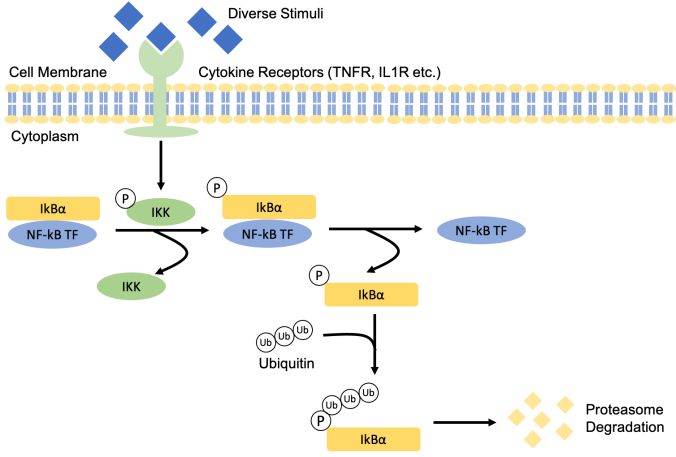
\includegraphics[scale=0.70]{NFkBactivation.png}
\caption{The binding of pro-inflammatory cytokines to its receptors triggers the activation of IKK which will phosphorylate IkB$\alpha$ releasing the sequestered NF-$\kappa$B Transcription Factor. The IkB$\alpha$ will then undergo proteasome degradation to synthesize new proteins. Image from \cite{Project}.}
\label{NFkBactivation}
\end{figure}

Although both IKK$\alpha$ and IKK$\beta$ are capable of phosphorylating I$\kappa$B$\alpha$ and I$\kappa$B$\beta$, they are less efficient kinase for
I$\kappa$B$\beta$ than for I$\kappa$B$\alpha$, and this difference may explain the delayed degradation kinetics of
I$\kappa$B$\beta$ following stimulation with Tumour Necrosis Factor (TNF)$\alpha$. This difference in degradation rate is in fact one of the characteristics of this I$\kappa$B member that was already mentioned in the previous section \ref{IkBs}.

IKK$\alpha$ and IKK$\beta$ dimerization are dependent on the \emph{leucine zipper domain}, which is therefore required for kinase activity.

Together with these two catalytic subunits, there is the regulatory
subunit \emph{NF-kB essential modifier} (\textbf{NEMO}-also known as IKK$\gamma$) which is not related to
IKK$\alpha$ and IKK$\beta$ and is characterized by a \emph{C-terminal zinc-finger like domain}, a \emph{leucine
zipper}, \emph{N-terminal and C-terminal coiled-coil domains}.

Both IKK$\alpha$ and IKK$\beta$ interact with NEMO through a C-terminal hexapeptide sequence termed the \emph{NEMO binding domain} (NBD).

Although in vitro assembly of the complex indicates that only IKK$\beta$ assembles with NEMO, data from IKK$\alpha$ knockout mice indicate instead that also IKK$\alpha$/NEMO
complexes are readily formed.

From here, the NF-$\kappa$B signaling pathways have been classified into two distinct and evolutionary
conserved types, according to the two multiprotein IKK complexes which regulate the stimulus-responsive phosphorylation and consequent degradation of I$\kappa$B proteins: the classical or so-called “canonical” NF-$\kappa$B signaling pathway where IKK$\beta$ is sufficient for I$\kappa$B$\alpha$ and
I$\kappa$B$\beta$ phosphorylation and degradation, while IKK$\alpha$ may regulate gene expression in the
nucleus by modifying the phosphorylation status of the histones.

On the contrary, in the
alternative or “non-canonical” pathway IKK complex consists exclusively of an IKK$\alpha$ homodimer, which leads to the phosphorylation of p100 and its consequent processing to p52.

Even though both classic and alternative pathways are principally activated during the functioning of the immune system, the first is mainly involved \emph{in inflammation response} as in the regulation of proliferation and apoptosis of lymphoid cells throughout the
immune reaction; the latter regulates the lymphoid organogenesis and so its engangement occurs mainly after non-inflammatory stimuli.





%NF-$\kappa$B dimers (mainly p50/p65, that is the major NF-$\kappa$B dimer of the canonical pathway, and p50/c-Rel) are consequently released and translocated to the nucleus to drive gene transcription of candidates involved in innate immunity, inflammation, proliferation, and survival (see figure \ref{NFkBmechanism}). 
  
%NF-$\kappa$B also activates transcription of the mRNA encoding its inhibitory subunit I$\kappa$B, thus generating a negative feedback circuit.

\begin{figure}[!ht]
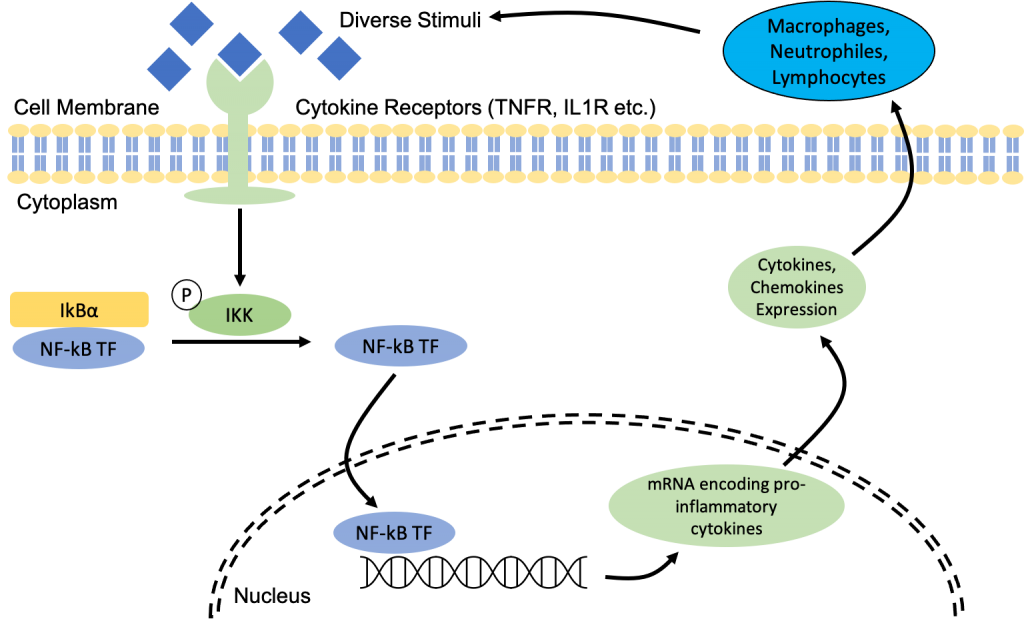
\includegraphics[scale=0.45]{NFkBmechanism.png}
\caption{Activation of canonical pathway during inflammation related to obesity. NF-$\kappa$B will induce transcription expression of pro-inflammatory cytokines when bound to DNA. Pro-inflammatory cytokines will recruit immune cells to the site. Presence of immune cells further produces pro-inflammatory cytokines which could bind to the cytokine receptors that are responsible for activating NF-$\kappa$B. Image from \cite{Project}.}
\label{NFkBmechanism}
\end{figure}
\newpage
%The ‘alternative’ or ‘non-classical’ NF-$\kappa$B-activating pathway is triggered by cytokines such as BAFF and lymphotoxin-b, and leads to the activation of an IKK$\alpha$ homodimer, which phosphorylates p100. This inhibitory molecule is subsequently processed to generate p52. NF-$\kappa$B dimers (p52/RelB) move into the nucleus to drive the expression of candidates involved in adaptive immunity, as well as in lymphoid organogenesis.
In the canonical pathway, after pathogen-derived lipopolysaccharide (LPS) mediates inflammatory stimulus and cytokines such as TNF and interleukin (IL)-1, , the I$\kappa$B proteins I$\kappa$B$\alpha$, I$\kappa$B$\beta$ and I$\kappa$B$\epsilon$ are phosphorylated by the “canonical” IKK complex on two specific N-terminal serines.

The subsequent ubiquitination mediated by the ubiquitin ligase $\beta$-TRCP makes I$\kappa$B available for
proteasomal degradation, so the NF-$\kappa$B dimers are capable to translocate in the nucleus and
activate gene transcription. This triggers transcription of the inhibitors and numerous other genes. Among the synthesized inhibitors, there are I$\kappa$B$\alpha$ and A20. The newly synthesized I$\kappa$B$\alpha$ again inhibits NF-$\kappa$B, while A20 inhibits IKK by catalysing its transformation into another inactive form (IKKi), in which it is no longer capable of phosphorylating I$\kappa$B$\alpha$.

Usually, NF-$\kappa$B activity can be detected within ten minutes after stimulation and some NF-$\kappa$B responsive promoters are induced almost immediately. As already mentioned, the activation of NF-$\kappa$B causes the transcriptional upregulation of I$\kappa$B$\alpha$ which causes \emph{a powerful negative feedback mechanism} that is responsible for the NF-$\kappa$B repression, whose activity can be restored after an other stimulus and may result in an oscillatory pattern of NF-$\kappa$B activity during chronic stimulation.

Conversely, multiple non-inflammatory stimuli are responsible for the engagement of the “non-canonical” pathway in a variety of cell types.

In B cells, the survival factor B-cell-activating factor belonging to the TNF family (BAFF) and, in splenic stromal cells, lymphotoxin $\beta$ signaling are able to activate NF-kB for many hours or days.

Although the activation mechanism remains partly unclear, it is thought that the precursor protein p100, which dimerizes with RelB, is partially processed to p52 upon IKK$\alpha$ activation by NF-$\kappa$B inducing kinase (NIK).

However, p100 processing was shown to be a co-translational mechanism, related to continuing p100 synthesis. Thus, p52 DNA-binding activity seems
delayed in comparison with p50/p65 complexes.

It is interesting to note that the non-canonical activation of NF-$\kappa$B is slower than canonical one, and it lacks a negative feedback control because the RelB-containing dimers are not subject to the high dynamic regulation of the I$\kappa$B proteins.

\begin{figure}[!ht]
\hspace*{-1cm} 
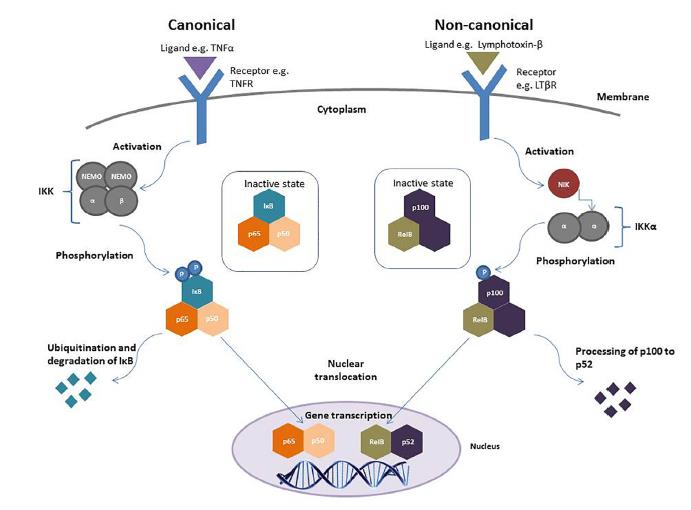
\includegraphics[scale=0.70]{canonicalvsnoncanonicalpathway.png}
\caption{Sketch of canonical vs non-canonical NF-$\kappa$B signaling pathway (Patel et al.,2018)}
\label{canonicalvsnoncanonicalpathway}
\end{figure}
\newpage



\section{Models of NF-\texorpdfstring{$\kappa$}{\265}B activity oscillations}
Many mathematical models of such key regulator NF-$\kappa$B activity oscillation have already been studied during years, highilighting the fact that it is  strongly regulated by the inhibitor protein I$\kappa$B$\alpha$. Here we list some studies results:
\begin{itemize}
 \item For the first time, a mathematical model was presented by Hoffman et al. Their research showed that the resulting negative feedback produces a propensity for oscillation in NF-$\kappa$B activity. 
 
 They analysed the I$\kappa$B-NF-$\kappa$B signaling module using knockout cell lines for the three I$\kappa$B isoforms (I$\kappa$B$\alpha$,I$\kappa$B$\beta$ and I$\kappa$B$\epsilon$) in order to evaluate the contribution of each one on the temporal
 control of NF-$\kappa$B oscillation.
 
 It was shown that the coordinated degradation, synthesis and localization of all three I$\kappa$B isoforms is required to generate the characteristic NF-$\kappa$B
 activation profile.
 
 \emph{The model displayed that I$\kappa$B$\alpha$ is responsible for strong negative feedback
 and a rapid switch-off of the NF-$\kappa$B response, while I$\kappa$B$\beta$ and $-\epsilon$ explained their action dampening the system's oscillatory potential and making stable the NF-$\kappa$B responses during longer stimulations.}
 
 \begin{figure}[!ht]
 \centering
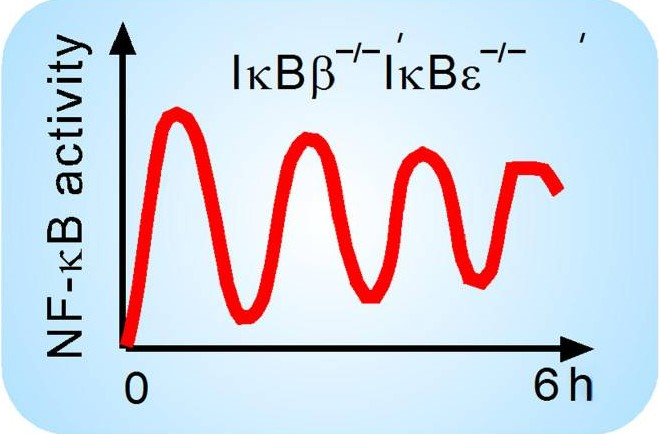
\includegraphics[scale=0.70]{NFkBOscillationProfileIkAlfa.jpg}
\caption{Schematic of oscillatory time course of NF-$\kappa$B in response to persistent TNF$\alpha$ in I$\kappa$B$\beta$ and I$\kappa$B$\epsilon$ knockout cells. Image from \cite{Hoffmanetal}.}
\label{NFkBOscillationProfileIkAlfa}
\end{figure}


 
 Moreover, the researchers identified a \emph{bimodal temporal I$\kappa$B-NF-$\kappa$B signaling behaviour depending on stimulus duration that is shown to generate also specificity in gene expression}.
 
\begin{figure}[!ht]
\centering
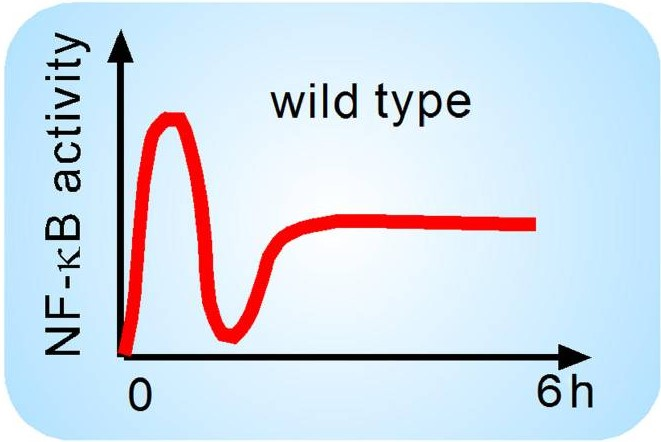
\includegraphics[scale=0.70]{NFkBTemporalBimodalProfile.jpg}
\caption{Characteristic biphasic time course of NF-$\kappa$B signaling in response to TNF$\alpha$ in various wild-type cells. NF-$\kappa$B activity peaks around 30 min, drops to basal levels around 1 h, and rises to an intermediate level thereafter \cite{Hoffmanetal}.}
\label{NFkBTemporalBimodalProfile}
\end{figure}
\newpage
 \item Based on this model, Kearns et al. explained better I$\kappa$B$\epsilon$ role, whose NF-$\kappa$B-induced transcription is delayed relative to that of I$\kappa$B$\alpha$. 
 
 I$\kappa$B$\epsilon$ delayed synthesis provided an antiphase negative feedback that effectively dampened I$\kappa$B$\alpha$ mediated oscillations.
 
 Furthermore, they demonstrated that both these negative feedback regulators are necessary for the termination of NF-$\kappa$B activity and NF-$\kappa$B mediated gene expression in response to transient stimuli.
 
 \item According to Mothes et al. and Wang et al., the oscillation was explained in detail through a bifurcation analysis; the models had two steady states, stable focus and unstable focus, with a stable limit cycle, depending on such bifurcation parameters which represented the intensity of the TNF$\alpha$ stimulation, total NF-$\kappa$B and I$\kappa$B$\alpha$ transcription rate.
 
 \item Inoue et al. mathematically analysed the NF-$\kappa$B oscillation by using the core model based on three components, IKK$\beta$, I$\kappa$B$\alpha$ and NF-$\kappa$B. According to their stability analysis, the NF-$\kappa$B activity showed two characteristic behaviours, \emph{oscillation and switch-like activation}, regulated by positive and negative feedback, respectively.
 
 Switch-like activation was fundamental to compensate for the upstream IKK transient activity and to induce accumulation of nuclear NF-$\kappa$B, which in turn was responsible for subsequent oscillation in target gene expression. %Lo possiamo modellizzare come un interruttore rappresentato da IKK che libera l'NF-kB dalla molecola inibitrice tramite fosforilazione e come un sistema oscillatorio nell'espressione prodotta dal gene, una volta che l'NF-kB è liberato e si attacca alla gene per farne la trascrizione.
 
 Thus, the NF-$\kappa$B oscillation was merely a damped oscillation.

\end{itemize}

However, the NF-$\kappa$B activity is neither a damped nor sustained oscillator phenomenon but is \emph{a stable transient event, in which different players are involved, such as RelA}.

The transcription of the NF-$\kappa$B target genes depends on the phosphorylation of both I$\kappa$B$\alpha$ and RelA subunit of NF-$\kappa$B, but no mathematical model considering RelA phosphorylation have been previously proposed.

So Hatanaka et.al constructed a model in which the focus was the influence of phosphorylation
of I$\kappa$B$\alpha$ and RelA on the nuclear-cytoplasmic oscillation.

They confirmed that NF-$\kappa$B signaling module transiently responded to the concentration of active IKK$\beta$ in a dependent manner. However, when the IKK$\beta$ concentration was fixed, the amplitude of the oscillation became larger as the value of total NF-$\kappa$B increased, suggesting that the oscillation period was regulated also by RelA phosphorylation.%Forse indica la liberazione del RelA grazie al IKKbeta.

Therefore, controlling the phosphorylation
process, it may be possible to govern the NF-$\kappa$B oscillation driving the NF-$\kappa$B dependent expression gene.


\section{NF-\texorpdfstring{$\kappa$}{\265}B and colorectal cancer}

As said at the beginning, NF-$\kappa$B proteins are involved in the control of a large number of normal cellular and organismal processes. However, on the other hand, these transcription factors are persistently active in a number of disease states, including cancer, arthritis, chronic inflammation, asthma, neurodegenerative diseases, and heart disease \cite{NFkB}. NF-$\kappa$B activation supports tumorigenesis by enhancing cell proliferation and angiogenesis, inhibiting apoptosis, and promoting cell invasion and metastasis.

No triggering mutations of NF-$\kappa$B in CRC have been described; however, constitutive activation of NF-$\kappa$B has been reported and is associated with higher tumor stages, treatment resistance and poor survival outcomes.

The role of NF-$\kappa$B in adenoma formation and development of colitis-associated cancer has been studied for the first time in a mouse model, where deletion of IKK$\beta$ in intestinal epithelial cell (IEC) and myeloid cells had distinct outcomes; deletion of IKK$\beta$ in IECs showed reduced adenoma incidence, which had a direct effect in tumor progression, as demonstrated by reduction in antiapoptotic B-cell lymphoma
2 (Bcl-2) protein, Bcl-$x_{L}$ . On the contrary, deletion of IKK$\beta$ in myeloid cells was associated with a less reduction in adenoma but showed reduced expression of genes encoding proinflammatory cytokines. So, the IKK$\beta$-mediated NF-$\beta$B activity has a cell-type specific role in the early-stage of carcinoma formation demostrating that the NF-$\kappa$B functions are cell-type and tumor-type specific.

However, no known studies have mapped NF-$\kappa$B expression in different human tissue concerning adenoma-carcinoma transformation. Furthers evidence demonstrate crosstalk between NF-$\kappa$B pathways and various other signaling networks implicated in CRC progression.

For example, growth factors can trigger the activation of the IKK complex through signaling pathways described in figure \ref{NFkBEGFR}.

\begin{figure}[!ht]
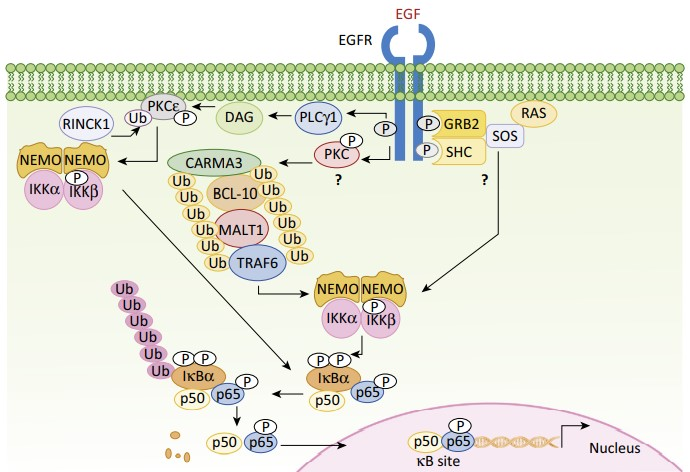
\includegraphics[scale=0.90]{EGFR.jpg}
\caption{Molecular mechanisms by which EGFR activates NF-kB. Image from \cite{EGFRNFkB}.}
\label{NFkBEGFR}
\end{figure}

Growth factor is a substance made by the body that functions to regulate cell division and cell survival \cite{GF}. Epidermal growth factor (EGF) is a protein that stimulates epidermal and epithelial cell growth and differentiation by binding to its receptor called Epidermal Growth Factor Receptor (EGFR) \cite{EGF}. The epidermal growth factor receptor is a transmembrane protein that is involved in cell signaling pathways that control cell division and survival \cite{EGFR}. Although it is now well established that EGF activates NF-$\kappa$B through the IKK complex, signaling molecules that link EGFR activation to the IKK complex have only been recently characterized.

In particular, constitutive epidermal growth factor receptor and nuclear factor $\kappa$b activities are seen in multiple solid tumors and combine to provide oncogenic signals to cancer cells. Recent studies have also defined mechanisms by which resistance occurs through crosstalk between EGFR- and NF-$\kappa$B-dependent pathways in colon cancer cells.






%METTI CAPITOLO TIPO NF-KB AS A PARTICULAR TOGGLE SWITCH.
\chapter{NF-\texorpdfstring{$\kappa$}{\265}B model formulation}

\part{Results and discussion}
%using experimental data del tuo centro di ricerca e di Hoffman.
%descrivi l'andamento nel tempo di quel che hai trovato teoricamente e di quello che ci si aspetta.
%sfrutta i metodi adottati nei circuiti genetici pi� semplici.

\chapter{Conclusions}\epigraph{``Frase''}{Autore}
%Per quanto riguarda l'algoritmo ibrido, occorrerebbe testarlo su tantissimi altri modelli e se ne ricaverebbe sicuramente miglioramento e automatizzare la scelta della differenza dei rate di soglia. Intanto per� abbiamo sviluppato un algoritmo che � ``adattativo'' nel senso che si applica il Tau-leap ed il Gillespie in base a quel che sono le dinamiche ed in un sistema come l'NF-kB in cui ci sono tanti tipi di reazione che si comportano in un modo o in un altro � quel che serve.
%Long-tail distributions governs biological systems and the ``queen'' of these is the Poisson Distribution.
%Metti nella conclusione della tesi che il tutto sta nel trovare i parametri giusti sia nel sistema che rappresenta il soggetto di questa tesi l'NF-kB per poterne modellizzare il comportamento e trovare terapie per tumori o infiammazioni croniche; sia nel percorso fatto per arrivare a studiare questo sistema allo scopo di ottenere i metodi giusti per poterlo esplorare. 
%Usiamo i metodi per esplorare la biologia per� vale anche il viceversa ossia la biologia stessa ci pu� aiutare a sviluppare i metodi come abbiamo fatto nell'algoritmo ibrido sfruttando le diverse configurazioni del modello ed i diversi tipi di regolazione.
%Quel che abbiamo definito e descritto come ``rumore'' in biologia all'inizio della tesi a livello computazionale lo si inserisce.
%Per quanto riguarda i modelli semplici analizzati: mentre nel caso del gene sempre espresso e regolato possiamo trovare situazioni generali in natura, nel caso dell'autorepressore ed il toggle switch non sembra per� nelle ricerche fatte in questo lavoro di tesi sembrano spesso essere coinvolti negli oncogenes e quindi casi di tumore. Anche l'NF-kB � un caso di gene sempre espresso per� non per garantire il buon funzionamento cellulare bens� � il caso in cui si ha un cattivo funzionamento.
\begin{appendices}
  \chapter{Software used in this thesis}
  All simulation methods and statistical data analysis have been performed using \emph{Python 3.9} and the programs are available in the following GitHub page \url{https://github.com/ManuelaCarriero/PyExTra} where you can find a detailed explanation of all the Python codes and how to reproduce the results reported in this work.
  \chapter{Glossary of biology}
  \begin{itemize}
   \item \textbf{Oncogenes} are genes that have the potential to cause cancer. In tumor cells, these genes are often mutated, or expressed at high levels \cite{oncogenes}.
   
    \item \textbf{Lymphoid cells} are a family of immune effector cells that have important roles in host defense, metabolic homeostasis and tissue repair but can also contribute to inflammatory diseases such as asthma and colitis \cite{lymphoidcellsnih}.
     
   \item \textbf{Lymphocyte} is a type of cell produced by lymphoid tissue that passes into the blood. It is one of the three elements of the white blood series and mediates the immune response by recognizing foreign molecules (antigens) with its membrane receptors; two main groups of lymphocytes are distinguished: the l. B which are responsible for the production of antibodies and the l. T which govern the destruction of cells infected by viruses and bacteria, foreign cells and tumor cells.
   \item \textbf{B lymphocyte} is type of white blood cell that makes antibodies. Also known as B cells, they are part of the immune system and develop from stem cells in the bone marrow \cite{NIHBCells}.
   \item A \textbf{knockout}, as related to genomics, refers to the use of genetic engineering to inactivate or remove one or more specific genes from an organism. Scientists create knockout organisms to study the impact of removing a gene from an organism, which often allows them to then learn something about that gene's function \cite{knockout}.
   \item \textbf{Interleukins} (IL) are a type of \emph{cytokine} (i.e. are a broad and loose category of small proteins $\sim5-20 kDa$ important in cell signaling) first thought to be expressed by leukocytes alone but have later been found to be produced by many other body cells. They play essential roles in the activation and differentiation of immune cells, as well as proliferation, maturation, migration, and adhesion. They also have pro-inflammatory and anti-inflammatory properties. The primary function of interleukins is, therefore, to modulate growth, differentiation, and activation during inflammatory and immune responses. Interleukins consist of a large group of proteins that can elicit many reactions in cells and tissues by binding to high-affinity receptors in cell surfaces. Interleukin 6 (\textbf{IL-6}) is an interleukin that acts as both a pro-inflammatory cytokine and an anti-inflammatory myokine (i.e. one of several hundred cytokines or other small proteins $\sim5-20 kDa$ that are produced and released by muscle fibers in response to muscular contractions). In humans, it is encoded by the IL6 gene.
   
   \item \textbf{Trans-inhibitor} is the catalytic inactivation of a homodimer, each of which subunits is catalytically active \cite{transinhibitorwikipedia}.
   
   \item \textbf{Tumor Necrosis Factor}
   
   \item \textbf{Phosphorylation}
   
   \item \textbf{Phenotypic Switching}
  
  \end{itemize}
\clearpage
\end{appendices}

%\addcontentsline{toc}{chapter}{Acknowledgments}
\chapter*{Acknowledgments}
\addcontentsline{toc}{chapter}{Acknowledgments} 
%we are all sons of the environment in which we live and so of the people with which we interact.
\begin{thebibliography}{bibliography}
     \bibitem{Brizi} Gastone Castellani, teaching material of {\em Physical Methods of Biology} course, University of Bologna.
    \bibitem{PR} Daniel Remondini, Gastone Castellani, teaching material of {\em Pattern Recognition} course, University of Bologna.
    \bibitem{SDAFAP} Claudia Sala, Maximiliano Sioli, teaching material of {\em Statistical Data Analysis for Applied Physics} course, University of Bologna.
    \bibitem{SACFAP} Enrico Giampieri, teaching material of {\em Software and Computing for Applied Physics} course, University of Bologna.
    \bibitem{PHD} Giampieri Enrico, {\em Stochastic models and dynamic meaures for the characterization of bistable circuits in cellular biophysics}, University of Bologna (2012).
    \bibitem{Tesi} Davide Giosué Lippolis, {\em Stochastic modeling of fluctuations in the NF-$\kappa$B activity of neoplastic cells}, University of Bologna (2018/2019).
    \bibitem{VanKampenBook} N. G. van Kampen, {\em Stochastic Processes in Physics and Chemistry}, North Holland, third ed., May 2007.
    \bibitem{Genetics} Yifeng Xia, Shen Shen, and Inder M. Verma, {\em NF-$\kappa$B, an active player in human cancers}, Cancer Immunol Res (2014) 2 (9): 823–830.
    \bibitem{NFkB} NF-kB Transcription Factors. URL \url{https://www.bu.edu/nf-kb/}.
    \bibitem{domain} Rel homology domain (RHD), DNA-binding domain. URL \url{https://www.ebi.ac.uk/interpro/entry/InterPro/IPR011539/}.
	\bibitem{Wiki} NF-kB. URL \url{https://en.wikipedia.org/wiki/NF-%CE%BAB}.
    \bibitem{Article} Tamás Székely Jr., Kevin Burrage, {\em Stochastic simulation in systems biology}, Computational and Structural Biotechnology Journal, Volume 12, Issues 20–21, November 2014, Pages 14-25.
    \bibitem{Method} Yang Cao, Daniel T. Gillespie and Linda Petzold, {\em Avoiding Negative Populations in Explicit Poisson Tau-Leaping}, Article  in  The Journal of Chemical Physics, September 2005.
    \bibitem{Project} INFLAMMATION'S ROLE IN OBESITY. URL \url{https://sites.tufts.edu/hkerstjaaalislai/?page_id=541}.
    \bibitem{EGFRNFkB} Kateryna Shostak and Alain Chariot, {\em EGFR and NF-kB: partners in cancer}, Trends in Molecular Medicine June 2015, Vol. 21, No. 6.
    \bibitem{YoutubeNFkB} NF-$\kappa$B pathways, Part 1: The canonical pathway of NF-$\kappa$B activation. URL \url{https://www.youtube.com/watch?v=7F_HPRfHdDk}.
    \bibitem{Definition} Genetic Heterogeneity. URL \href{https://www.sciencedirect.com/topics/biochemistry-genetics-and-molecular-biology/genetic-heterogeneity}{https://www.sciencedirect.com/}
    \bibitem{EGFR} epidermal growth factor receptor. URL \href{https://www.cancer.gov/publications/dictionaries/cancer-terms/def/epidermal-growth-factor-receptor}{https://www.cancer.gov}
    \bibitem{GF} growth factor. URL \href{https://www.cancer.gov/publications/dictionaries/cancer-terms/def/growth-factor}{https://www.cancer.gov}
    \bibitem{EGF} Epidermal growth factor. URL \href{https://en.wikipedia.org/wiki/Epidermal_growth_factor}{https://en.wikipedia.org}
    \bibitem{Math} N. G. van Kampen, {\em Stochastic Processes in Physics and Chemistry}, North Holland, third ed., May 2007.
    \bibitem{ACF} Autocorrelation Function. URL \href{https://www.sciencedirect.com/topics/chemistry/autocorrelation-function#:~:text=1%20Autocorrelation-,The%20autocorrelation%20function%20(ACF)%20defines%20how%20data%20points%20in%20a,signal%20over%20different%20delay%20times.}{https://www.sciencedirect.com}
    \bibitem{Stat} G. Cowan, {\em Statistical Data Analysis}, Oxford University Press Inc., New York, 1998.
    \bibitem{onesteparticle} Mathisca de Gunst, Michel Mandjes and Birgit Sollie, {\em Statistical inference for a quasi birth–death model of RNA transcription}, BMC Bioinformatics 23, 105 (2022).
    \bibitem{Hand} C.W.Gardiner, {\em Handbook of Stochastic Methods for Physics, Chemistry and the Natural Sciences}, Printed in Germany, Springer-Verlag Berlin Heidelberg 1983,1985.
    \bibitem{Ragazza} Luciana Renata De Oliveira, {\em Master Equation: Biological Applications and Thermodynamic Description}, University of Bologna (2013/2014).
     \bibitem{WaveletsTutorial} A guide for using the Wavelet Transform in Machine Learning. URL \href{https://ataspinar.com/2018/12/21/a-guide-for-using-the-wavelet-transform-in-machine-learning/}{https://ataspinar.com}
    \bibitem{ScienceDirectMorlet} Morlet Wavelet. URL \href{https://www.sciencedirect.com/topics/mathematics/morlet-wavelet}{https://www.sciencedirect.com}
    \bibitem{Neuroscience} Michael X Cohen, {\em A better way to define and describe Morlet wavelets
    for time-frequency analysis},Radboud University and Radboud University Medical Center; Donders Institute for Neuroscience.
    \bibitem{UsefullYoutube} Wavelets: a mathematical microscope. URL \href{https://www.youtube.com/watch?v=jnxqHcObNK4&t=1320s}{https://www.youtube.com}
    \bibitem{Immuno} Yoshiteru Sasaki, Kazuhiro Iwai, {\em Roles of the NF-$\kappa$B Pathway in B-Lymphocyte Biology}, Curr Top Microbiol Immunol. 2016;393:177-209.
    \bibitem{immunoglobulin} Immunoglobulin Light Chain. URL \href{https://www.sciencedirect.com/topics/immunology-and-microbiology/immunoglobulin-light-chain}{https://www.sciencedirect.com}
    %\bibitem{Exp} Baeuerle, P. A. Baltimore, D. A 65-kappaD subunit of active NF-kappaB is required for inhibition of NF-kappaB by I kappaB. Genes Dev. 3, 1689–1698 (1989).
    \bibitem{Ankyrin} Kumar A, Balbach J., {\em Folding and Stability of Ankyrin Repeats Control Biological Protein Function}. Biomolecules. 2021 Jun 5;11(6):840. doi: 10.3390/biom11060840. PMID: 34198779; PMCID: PMC8229355.
    \bibitem{AnkyrinMotif} Li J, Mahajan A, Tsai MD., {\em Ankyrin repeat: a unique motif mediating protein-protein interactions}. Biochemistry. 2006 Dec 26;45(51):15168-78. doi: 10.1021/bi062188q. PMID: 17176038.
    \bibitem{hematopoieticNIH} hematopoietic stem cell. URL \href{https://www.cancer.gov/publications/dictionaries/cancer-terms/def/hematopoietic-stem-cell}{https://www.cancer.gov}
    \bibitem{knockout} Knockout. URL \href{https://www.genome.gov/genetics-glossary/Knockout}{https://www.genome.gov}
    \bibitem{lymphoidcellsnih} Zook EC, Kee BL., {\em Development of innate lymphoid cells}. Nat Immunol. 2016 Jun 21;17(7):775-82. doi: 10.1038/ni.3481. PMID: 27328007.
    \bibitem{transinhibitorwikipedia} transinhibition. URL \href{https://en.wiktionary.org/wiki/transinhibition}{https://en.wiktionary.org}
    \bibitem{NIHBCells} B cell. URL \href{https://www.cancer.gov/publications/dictionaries/cancer-terms/def/b-cell}{https://www.cancer.gov}
    \bibitem{Hoffmanetal} Cheong R, Hoffmann A, Levchenko A., {\em Understanding NF-kappaB signaling via mathematical modeling}. Mol Syst Biol. 2008;4:192.
    \bibitem{datadrivenmodeling} Ch. Venkateswarlu, Rama Rao Karri, {\em Optimal State Estimation for Process Monitoring, Fault Diagnosis and Control}, Chapter 5 - Data-driven modeling techniques for state estimation, Elsevier, 2022, Pages 91-111.
    \bibitem{GeneticHeterogeneity} Genetic Heterogeneity. \href{https://en.wikipedia.org/wiki/Genetic_heterogeneity}{https://en.wikipedia.org}
    \bibitem{genotypevsphenotype} M. Manceau, V.S. Domingues, C.R. Linnen, E.B. Rosenblum, H.E. Hoekstra, {\em Convergence in pigmentation at multiple levels: mutations, genes and function}. Phil Trans R Soc B, 365 (2010), pp. 2439-2450.
    \bibitem{heterogeneityinclones} D. Stockholm, R. Benchaouir, J. Picot, P. Rameau, T.M.A. Neildez, G. Landini, et al., {\em The origin of phenotypic heterogeneity in a clonal cell population in vitro}. PLoS One, 2 (2007), p. e394.
    \bibitem{intrinsic} Close J.L. Spudich, D.E. Koshland Jr., {\em Non-genetic individuality: chance in the single cell}. Nature, 262 (1976), pp. 467-471.
    \bibitem{geneexpressionnoise} Munsky B, Neuert G, van Oudenaarden A.,{\em Using gene expression noise to understand gene regulation}. Science. 2012 Apr 13;336(6078):183-7. 
    \bibitem{adaptivenoise} M. Viney, S.E. Reece, {\em Adaptive noise}. Proc R Soc B, 280 (2013), p. 20131104.
    \bibitem{noisewithabundance} A. Bar-Even, J. Paulsson, N. Maheshri, M. Carmi, E. O'Shea, Y. Pilpel, et al., {\em Noise in protein expression scales with natural protein abundance}. Nat Genet, 38 (2006), pp. 636-643.
    \bibitem{SanDiegoUniversity} Matt Scott, {\em Tutorial: Genetic circuits and noise}. Quantitative Approaches to Gene Regulatory Systems. Summer School, July 2006. University of California, San Diego.
    \bibitem{housekeepinggene} Housekeeping gene \href{https://en.wikipedia.org/wiki/Housekeeping_gene}{https://en.wikipedia.org}
    \bibitem{yeastexperiments} Zenklusen D, Larson DR, Singer RH. {\em Single-RNA counting reveals alternative modes of gene expression in yeast}. Nat Struct Mol Biol. 2008 Dec;15(12):1263-71. 
    \bibitem{generegulationNIH} Gene regulation. \href{https://www.genome.gov/genetics-glossary/Gene-Regulation}{https://www.genome.gov}
    \bibitem{RFX1Gene} RFX1 Gene - Regulatory Factor X1 \href{https://www.genecards.org/cgi-bin/carddisp.pl?gene=RFX1}{https://www.genecards.org}
    \bibitem{RFX1ArsenalAgainstCancer}
    Issac, J., Raveendran, P.S. Das, A.V., {\em RFX1: a promising therapeutic arsenal against cancer}. Cancer Cell Int 21, 253 (2021). 
    \bibitem{RFX1genehumansyeast}    
    Lubelsky Y, Reuven N, Shaul Y.,{\em Autorepression of rfx1 gene expression: functional conservation from yeast to humans in response to DNA replication arrest}. Mol Cell Biol. 2005 Dec;25(23):10665-73.
    \bibitem{microRNAs} Giampieri E, Remondini D, de Oliveira L, Castellani G, Li\'o P., {\em Stochastic analysis of a miRNA-protein toggle switch}. Mol Biosyst. 2011 Oct;7(10):2796-803.
    \bibitem{AssocProfThamer} Random Process (or Stochastic Process) \href{https://uotechnology.edu.iq/dep/coe/lectures/dr-THAMER/Probability%20&%20Statistics/ch%203.pdf}{https://uotechnology.edu.iq}
    \bibitem{nfkb30years} Zhang Q, Lenardo MJ, Baltimore D., {\em 30 Years of NF-?B: A Blossoming of Relevance to Human Pathobiology}. Cell. 2017 Jan 12;168(1-2):37-57.
    \bibitem{oncogenes} Oncogene \href{https://en.wikipedia.org/wiki/Oncogene}{https://en.wikipedia.org}
    \bibitem{Manuel} Manuel D. Rossetti, {\em Simulation Modeling and Arena}. \url{https://rossetti.github.io/RossettiArenaBook/}
    \bibitem{RungeKutta} Runge Kutta methods \url{https://en.wikipedia.org/wiki/Runge-Kutta_methods}

\end{thebibliography}
%\addcontentsline{toc}{chapter}{Bibliography}









\end{document}

